% todo: March 18:
% 2. add number of relations to databases.
% 3. Change terminology to Functor Bayes net. reasons: ``parametrized'' is missing parameters. (2) not ground. (3) follow previous papers.
%%%%%%%%%%%%%%%%
%1.check functor Bayes net terminology vs. functor Bayes net. Avoid when possible.
% 2. check uses of ``semantics''. How about doing both. Set it up in background.
% 3. change citation of DRC to Gehre, vs. join tuples for SRMs. 
% 4. add MLN experiments.-> audience comment! also, what about MLN queries with 1st-order variables.
% 5. add synthetic data.
% 6. template has 1st-order variables, but is just a conceptual aid. Don't query it.
% 7. class-level Is like asking an aggregate query about nodes, see lifted inference. Lifted inference parfactors are mixed. Computed on the fly. Means to end, where the end is probability for an individual. Halpern and Russell on probabilities over worlds vs nodes.
% 8. Check Lise's thesis for diff between SRM and PRM.
%9. Closed-world assumption, see BLOG, missing data. Sampling assumptions. Does 1-minus trick assume closed-world, no missing data? Not active learning. Separate statistical from computational questions: if you had a model of how false vs. unknown links relate, we could extend it. Maybe point to boosting work. Who asked this?

\documentclass[oribibl]{llncs}
%Example for automatically rescaling equations. 
% This is very tricky.
%\begin{equation}
%\label{eq:pimax}
%\resizebox{.55\textwidth}{!}{$
%\begin{split}
%P(\jtable_{2}|\set{E},\ttable) \propto &
%P(\keys = [jack,101],\it{Gr} = A, \it{Sat} = 1|\it{Int} = \class, \it{Rank} = 1, \it{Rat} = 3, \it{Diff}=1)\\
%\times & P(\keys = [jack,102],\it{Gr} = B, \it{Sat} = 2|\it{Int} = \class, \it{Rank} = 1, \it{Rat} = 2, \it{Diff}=2).
%\end{split}$
%}
%\end{equation}

%\usepackage{times}
%\usepackage[normaltitle,normalbib,normalmargins,normalindent]{savetrees}
\usepackage{amsmath}
\usepackage{amsfonts}
\usepackage{amssymb}
\usepackage{graphicx}
\usepackage{url}
%\usepackage{subfigure}
\usepackage{epstopdf}
\setcounter{MaxMatrixCols}{30}
%\usepackage{algorithm}
%\usepackage{algorithmic}
\usepackage{subfigure}
%\usepackage{subcaption}
\usepackage{fancyhdr}
\graphicspath{{../}{figures/}}
\usepackage{todonotes}

\DeclareMathOperator*{\argmax}{argmax}
\DeclareMathOperator*{\argmin}{argmin}
%\DeclareMathOperator{\pattern}{\pi}
\DeclareMathOperator{\Poly}{\mathbf{\mathrm{P}}}
\DeclareMathOperator{\RP}{\mathbf{\mathrm{RP}}}
%\DeclareMathOperator{\FP}{\mathbf{\mathrm{FP}}}
\DeclareMathOperator{\NP}{\mathbf{\mathrm{NP}}}
%\DeclareMathOperator{\E}{\mathbb{E}}
\renewcommand{\d}{\mathbf{d}}

\newcommand{\ZZ}{\mathbf{Z}}

\newcommand{\indep}{\ensuremath{\perp{}\!\!\!\!\!\!\!\perp{}}}
\newcommand{\dep}{\ensuremath{{\perp{}\!\!\!\!\!\!\!\not  \perp{}}}}
%\renewcommand{\L}{\mathcal{L}}
% variables denoting sets of nodes
\newcommand{\V}{V} 
\newcommand{\partC}{\mathcal{C}}
\newcommand{\pattern}{\pi}
% variables denoting nodes
\newcommand{\B}{B}
\renewcommand{\P}{P}
\newcommand{\R}{R}
\newcommand{\X}{X}
\newcommand{\Y}{Y}
\newcommand{\Z}{Z}
\newcommand{\F}{F}
\newcommand{\U}{U}
\newcommand{\W}{W}
\renewcommand{\S}{S}
\newcommand{\C}{C}
\newtheorem{mydef}{Proposition}
%variables for values
%\newcommand{\u}{u}
\renewcommand{\a}{a}
\renewcommand{\b}{b}
\newcommand{\z}{z}
\renewcommand{\v}{v}
\newcommand{\x}{x}
\newcommand{\y}{y}
\newcommand{\p}{p}
\newcommand{\s}{s}
\newcommand{\w}{w} % weights


%statistics
\newcommand{\divergence}{\it{D}}
\newcommand{\score}{\it{score}}
\newcommand{\confidence}{\it{conf}}
\newcommand{\support}{\it{support}}
\newcommand{\loglikelihood}{\it{LOG}}
\newcommand{\lof}{\it{LOF}}
\newcommand{\llmetric}{-L}
\newcommand{\lr}{\it{LR}}
\newcommand{\kl}{\it{KL}}
\newcommand{\el}{\it{EL}}
\newcommand{\mi}{\it{MI}}
\renewcommand{\mid}{\it{ELD}}
\newcommand{\jid}{\it{JID}}
\newcommand{\roc}{\it{ROC}}
\newcommand{\outrank}{\it{OutRank}}
\newcommand{\knn}{\it{KNNOutlier}}
\newcommand{\auc}{\it{AUC}}
\newcommand{\eld}{\it{ELD}}
\newcommand{\fd}{\it{FD}}
\newcommand{\parameter}{\theta}
\newcommand{\parameters}{\bs{\parameter}}
\newcommand{\bic}{\mathit{BIC}}
%random variables and graphical models
% number of values in the domain of a random variable
% variables for BNs
\newcommand{\domvals}{k}
\newcommand{\nodevalue}{\v}
\newcommand{\parvalue}{\mathbf{\pi}} % a single assignment of values to a set of 
%parents
\newcommand{\parvals}{l} % number of values of parent state.
\renewcommand{\r}{r} % CP-table row
\newcommand{\nbhd}{{\mathsf {nbdh}}}
\newcommand{\child}{\mathit{child}}
\newcommand{\parent}{\mathit{pa}}
\newcommand{\parents}{\mathbf{pa}}
\newcommand{\Parents}{\mathbf{PA}}
\newcommand{\family}{F} % families, family formulas
\newcommand{\vpi}{\mathbf{pa}} % for vectors of variable assignments
\renewcommand{\l}{\ell} % class label
\newcommand{\states}{r} % number of states of a variable
%\newcommand{\value}{value}
\newcommand{\mb}{\set{mb}} % markov blanket of a variable, vector-valued
\newcommand{\ssize}{N} % number of rows in join table; size of sample
\newcommand{\mbstates}{m} % number of states in Markov blanket
\newcommand{\frequency}{fr}
\newcommand{\pseudo}{\ast}
\newcommand{\counts}{+}
\newcommand{\weighted}{\ast}
\newcommand{\halpern}{H}
\newcommand{\Thetaa}{\theta}
\newcommand{\instance}{I}

%logic notation
%\newcommand{\predicate}{\phi}
\newcommand{\functor}{f}
\newcommand{\outdomain}{V}
\newcommand{\indomain}{\Omega}
\newcommand{\variable}{X} % first-order variable
\newcommand{\population}{\mathcal{P}}
\newcommand{\entity}{x}
\newcommand{\formula}{\phi}
\newcommand{\formulas}{\mathcal{\phi}}
\newcommand{\literal}{l}
\newcommand{\conjunction}{\set{C}} % conjunction of literals
\newcommand{\fterm}{\f} % open function term
\newcommand{\fterms}{F} % set of function terms, also nodes in JBN
\newcommand{\term}{\sigma}
\newcommand{\Terms}{\bs{\sigma}}
\newcommand{\constant}{a}
\newcommand{\constants}{\bs{\constant}}
\newcommand{\gterm}{g} % ground term
\newcommand{\gterms}{\bs{\gterm}} %list of ground terms
\newcommand{\vterm}{x} % variable term
\newcommand{\vterms}{\bs{\vterm}} % list of variable terms
\newcommand{\assign}{A} % assignment of values to Bayes net
\newcommand{\resultset}{\mathbb{R}}
\newcommand{\grounds}{\#}
\newcommand{\grounding}{\gamma}
\newcommand{\groundall}{\Gamma}
\newcommand{\vars}{\mathit{Var}} % variables in a conjunction
\newcommand{\igraph}{I} % instance-level dependency graph.
\newcommand{\assignment}{\set{a}}
\newcommand{\atom}{\ell}
\newcommand{\gnode}{\alpha}
\newcommand{\gfamily}{\ground{f}}
\newcommand{\numformulas}{m}
\newcommand{\structure}{\mathcal{S}}
% logic programs
\newcommand{\program}{\mathcal{B}}
\newcommand{\clause}{\mathcal{c}}
\newcommand{\head}{\mathit{head}}
\newcommand{\body}{\mathit{body}}
\newcommand{\crule}{\mathit{cr}} % combining rule
\newcommand{\level}{\mathit{level}} % rank of function symbols in LP

%datbase schema
\newcommand{\rcolumns}{R}
\newcommand{\ecolumns}{E}
\newcommand{\dtable}{T} % can't use \table. Generic database table
\newcommand{\datatable}{D} % generic data table, not necessarily part of database.
\newcommand{\jtable}{J} % join table
\newcommand{\Ejoin}{$J^{+}$}
\newcommand{\jtables}{m}
\newcommand{\rtable}{R} % relationship table
\newcommand{\etable}{E} % entity table.
\newcommand{\ttable}{X} % target table
\newcommand{\nextended}{n}
\newcommand{\row}{r}
\newcommand{\rows}{\mathit{rows}}
\newcommand{\col}{j}
\newcommand{\cols}{\mathit{cols}}
\newcommand{\unary}{\f} % to denote a unary or attribute function
\newcommand{\numatts}{u} % to denote the number of unary or attribute functions.
\newcommand{\g}{g} % alternative for function
\newcommand{\relational}{\mathbf{r}} % denotes a generic relational functors, can be both relationship or descriptive attribute of relationship
\newcommand{\Relation}{R} % denotes a generic boolean relation
% a special type of literal conjunction that assigns a value %to each variable
\providecommand{\keywords}{\textbf{keywords: }}
\newcommand{\loss}{\ell}
\newcommand{\class}{c} % the class attribute
\newcommand{\classlabel}{y} % the class label
\newcommand{\classifier}{\mathcal{M}}
\newcommand{\target}{t} % target object
\newcommand{\Target}{T}
\newcommand*\rfrac[2]{{}^{#1}\!/_{#2}}
\newcommand{\object}{o}
\newcommand{\Class}{C}
\newcommand{\scorediff}{\Delta}
\newcommand{\model}{B}
\newcommand{\modelprob}{\theta}
\newcommand{\profile}{P}
% the probabilities defined by a model, like conditional probabilities in a BN
\newcommand{\Targetcount}{\Gamma}
\newcommand{\neighbor}{n}
\newcommand{\feature}{V} % feature or desc attribute of object or link
\newcommand{\features}{\bs{v}} % features 
\newcommand{\Features}{\bs{V}}
\newcommand{\attribute}{a} % nonclass attribute of target object
\newcommand{\attributes}{\bs{a}}
\newcommand{\rels}{\bs{R}} % chain of relationships.
\newcommand{\maxpath}{\rho}
\newcommand{\eatts}{\it{1Nodes}}
\newcommand{\ratts}{\it{2Nodes}}
\newcommand{\atts}{\it{ANodes}}
\newcommand{\marginalize}{\it{margin}}
%special functions
\newcommand{\AVG}{\it{AVG}}
\newcommand{\instances}{n} % counts number of occurrences in DB
\newcommand{\prob}{p} % frequency of formula true in in DB

%variables denoting graphs or models
\newcommand{\mln}{M}
\newcommand{\G}{G}
\newcommand{\node}{V}
\newcommand{\nodes}{V}
\newcommand{\edges}{E}
\newcommand{\clique}{C}
\newcommand{\cliques}{\mathcal{\clique}}
\newcommand{\cliquevalue}{c}
\newcommand{\graph}{G}
\newcommand{\M}{M}
\newcommand{\J}{J}
\renewcommand{\H}{H}
\newcommand{\K}{K} % component
\renewcommand{\O}{O} % oracle
\renewcommand{\path}{\rho} % path, also foreignkey path
% Markov nets
\newcommand{\potential}{\Psi}
% database schema
\newcommand{\type}{\tau} % to denote a generic type
\newcommand{\E}{E} % for entity tables
\newcommand{\e}{e} % for specific entities
\newcommand{\f}{f}
\newcommand{\new}{\it{new}}
\renewcommand{\c}{c}
\renewcommand{\R}{R} % for relationship tables
\newcommand{\A}{A} % for attributes
\newcommand{\T}{T} % for tables generically
\newcommand{\New}{N}
\newcommand{\D}{\mathcal{D}} % for database instance
\newcommand{\databases}{\set{D}} % the number of databases
\newcommand{\vocab}{\mathcal{\L}} % for logical vocabulary associated with database
\newcommand{\name}{\mathit{name}} % generic attribute
\newcommand{\dom}{\mathit{dom}} % domain of attributes
\newcommand{\etables}{\alpha} % entity tables
\newcommand{\rtables}{\beta} % relationship table number
% specific constructs for examples


\newcommand{\team}{\it{T}}
\newcommand{\player}{\it{P}}
\newcommand{\match}{\it{M}}


\newcommand{\director}{\it{Director}}
\newcommand{\movie}{\it{Movie}}
\newcommand{\user}{\it{User}}
\newcommand{\corr}{\it{\rho}}
\newcommand{\student}{\mathit{Student}}
\newcommand{\I}{\mathit{I}}
\newcommand{\course}{\mathit{Course}}
\newcommand{\prof}{\mathit{Professor}}
\newcommand{\person}{\mathit{Person}}
\newcommand{\TA}{\mathit{TA}}
\newcommand{\actor}{\mathit{Actor}}
\newcommand{\age}{\mathit{age}}
\newcommand{\intelligence}{\mathit{intelligence}}
\newcommand{\diff}{\mathit{difficulty}}
\newcommand{\reg}{\mathit{Registered}}
\newcommand{\win}{\it{win}}
\newcommand{\ra}{\mathit{RA}}
\newcommand{\bt}{\mathit{blood type}}
\newcommand{\grade}{\mathit{grade}}
\newcommand{\gpa}{\mathit{gpa}}
\newcommand{\jack}{\mathit{Jack}}
\newcommand{\jill}{\mathit{Jill}}
\newcommand{\smith}{\mathit{Smith}}
\newcommand{\cmpt}{\mathit{CMPT120}}
\newcommand{\hi}{\mathit{Hi}}
% various constants
\newcommand{\true}{\mathit{T}}
\newcommand{\false}{\mathit{F}}
\newcommand{\normalconstant}{Z} % the normalization constant

% orderings
\newcommand{\pred}{\mathit{pred}}
%procedure names and such
\newcommand{\join}{\textsc{Join-Frequencies}}
\newcommand{\linus}{\textsc{Linus }}
\newcommand{\foil}{\textsc{Foil }}
\newcommand{\MLN}{\textsc{MLN}}
\newcommand{\treetilde}{\textsc{TILDE }}

%%%
%undirected models
\newcommand{\pot}{\phi} % potential function
%\newcommand{\theHalgorithm}{\arabic{algorithm}}
\newcommand{\test}{test}
\def\set#1{\mathbf{#1}}
\def\bs#1{\boldsymbol{#1}}
\def\ground#1{\overline{#1}}


\graphicspath{{../../}{figures/}}

\begin{document}
%\usepackage{url}
%\usepackage{natbib}
%\usepackage{hyperref}

\newcommand{\theHalgorithm}{\arabic{algorithm}}

\title{Modelling Relational Statistics With Bayes Nets}
\institute{School of Computing Science,   Simon Fraser University,\\ Burnaby, British Columbia, Canada 
%\email{bba18,oschulte@cs.sfu.ca}
}


\author{Oliver Schulte \and Hassan Khosravi \and Arthur E. Kirkpatrick \and Tianxiang Gao \and Yuke Zhu}
\maketitle  


\begin{abstract} 
Class-level models capture relational statistics over object attributes and their connecting links, answering questions such as ``what is the percentage of friendship pairs where both friends are women?'' Class-level relationships are important in themselves, and they support applications like policy making, strategic planning, and query optimization. We represent class statistics using Parametrized Bayes Nets (PBNs), a first-order logic extension of Bayes nets. Queries about classes require a new semantics for PBNs, as the standard grounding semantics is only appropriate for answering queries about specific ground facts. We propose a novel random selection semantics for PBNs, which does not make reference to a ground model, and supports class-level queries.
%, based on Halpern's classic random selection semantics for probabilistic first-order logic \cite{Halpern90}. 
The parameters for this semantics can be learned using the recent  pseudo-likelihood measure \cite{Schulte2011} as the objective function. This objective function is maximized by taking the empirical frequencies in the relational data as the parameter settings. We render the computation of these empirical frequencies tractable in the presence of negated relations by the inverse M\"obius transform. Evaluation of our method on four benchmark datasets shows that maximum pseudo-likelihood provides fast and accurate estimates at different sample sizes.  
\end{abstract}

%\begin{abstract}
%Relational and network data are very common, but raise statistical challenges because of dependencies among links and linked units. 
%%One of the goals of statistical-relational learning is to extend machine learning techniques, such as Bayes net learning, for relational data. 
%Recent work has utilized a relational pseudo-likelihood measure to develop effective Bayes structure learning algorithms. This paper uses the pseudo-likelihood measure for parameter learning. We compare classic maximum likelihood estimation for nonrelational data (MLE) with maximum pseudo-likelihood estimation (MPLE) for relational data, with respect to three properties. (1) Consistency. Given an infinitely large data sample, both MLE and MPLE converge to the asymptotic frequencies. (2) Asymptotic efficiency. Whereas MLE is known to achieve minimum variance in the sample size limit, the efficiency of MPLE can be reduced due to data dependencies. (3) Computational Tractability. Computing sufficient statistics in a relational database is difficult when the statistics involve negated links.
% %(e.g., users who are not friends with each other). 
% We present a novel application of the inverse M\"obius transform for solving this problem.
%\end{abstract}

%\begin{abstract}
%Data are commonly stored in relational or network form.  This form 
%raises statistical challenges because the links and linked units are statistically dependent.
%%One of the goals of statistical-relational learning is to extend machine learning techniques, such as Bayes net learning, for relational data. 
%%Recent work has utilized a relational pseudo-likelihood measure to develop effective Bayes structure learning algorithms.
%{\em Connection between MPLE and statistically dependent data?}
%This paper applies a pseudo-likelihood measure for parameter learning in Bayes net representations of relational data. We compare classic maximum likelihood estimation for nonrelational data (MLE) with maximum pseudo-likelihood estimation (MPLE) for relational data, with respect to three properties: (1) Consistency. Given an infinitely large data sample, both MLE and MPLE converge to the asymptotic frequencies. (2) Asymptotic efficiency. Whereas MLE is known to achieve maximum efficiency in the sample size limit, the efficiency of MPLE can be lower due to data dependencies. (3) Computational Tractability. Computing sufficient statistics in a relational database is difficult when the statistics involve negated links.
% %(e.g., users who are not friends with each other). 
% We present an application of the inverse M\"obius transform for computing MPLE efficiently for negated links.
%{\em Benefits of having this MPLE?}  {\em Comparison of MLE tractability and MPLE tractability?}
%\end{abstract}

%\begin{abstract}
%Data are commonly stored in relational or network form. Learning statistical patterns based on relational frequencies is an important machine learning tasks that supports applications like policy making, strategic planning, and query optimization. Bayes nets (BNs) are a widely used generative model class for representing statistical patterns. A standard BN parameter learning method is classic maximum likelihood estimation (MLE). Applying MLE to relational data runs into the well-known problem that  defining a relational likelihood function for a BN model is difficult due to cyclic relational dependencies \cite{Domingos2007,Taskar2002,Neville2007,Getoor2007c}. A BN pseudo-likelihood measure for relational data was recently introduced to replace the standard product likelihood for single-table data \cite{Schulte2011}.
%We compare classic MLE for nonrelational data with maximum pseudo-likelihood estimation (MPLE) for relational data, with respect to three properties: (1) Consistency. Given an infinitely large data sample, both MLE and MPLE converge to the asymptotic frequencies. (2) Asymptotic efficiency. Whereas MLE is known to achieve minimum variance in the sample size limit, the efficiency of MPLE can be lower due to data dependencies. (3) Computational Tractability. Whereas MLE requires only simple row counts, computing sufficient statistics in a relational database is difficult when the statistics involve negated links (e.g., users who are not friends with each other). 
% We present an application of the inverse M\"obius transform for computing MPLE efficiently for negated links.
%{\em Benefits of having this MPLE?}  {\em Comparison of MLE tractability and MPLE tractability?}
%\end{abstract}
%\begin{abstract} 
%Class-level dependencies model general relational statistics over attributes of linked objects and links. Class-level relationships are important in themselves, and they support applications like policy making, strategic planning, and query optimization. An example of a class-level query is ``what is the percentage of friendship pairs where both are women?''. To represent class-level statistics, we utilize
%functor Bayes nets (PBNs), a first-order logic extension of Bayes nets. The standard grounding semantics for PBNs is appropriate for answering queries about specific ground facts
% %("what is the probability that Tweety can fly?") 
% but not appropriate for answering queries about classes of individuals.
% %("What percentage of birds fly?"), 
% %that concern generic statistical information about the whole population. 
%We propose a random selection semantics for PBNs, based on Halpern's classic semantics for probabilistic first-order logic \cite{Halpern90}, that supports class-level queries. Learning the parameters for this semantics can be done using the recent relational BN pseudo-likelihood measure \cite{Schulte2011} as the objective function.
%%, which like Halpern's semantics is based on random instantiations of first-order variables. 
%The parameter settings that maximize this objective function are the empirical frequencies in the relational data. 
%%Bayes net parameters are often learned using classic maximum
%%likelihood estimation (MLE). Applying MLE to relational data is difficult,
%%however, due to the dependencies introduced by cyclic relationships~\cite{Domingos2007,Taskar2002,Neville2007,Getoor2007c}. 
%%%\cite{Domingos2007,Taskar2002,Neville2007,Getoor2007c}. 
%%To address cyclic relations, a BN pseudo-likelihood measure was
%%recently introduced for relational data \cite{Schulte2011}.
%%This measure can be used to construct maximum pseudo-likelihood estimation (MPLE)
%%for estimating BN parameters.
%%A naive implementation is intractable due to the
%A naive computation of the empirical frequencies of the relations is intractable due to the complexity imposed by negated relations. %al links. 
%We render
%the computation tractable by using the inverse M\"obius
%transform. Evaluation on four benchmark datasets shows that 
%%MPLE is consistent, and 
%maximum pseudo-likelihood provides accurate estimates at different sample sizes.  
%TIME, ACCURACY?
%, and is statistically consistent in the sense of approaching the correct parameter value with increasing sample size.
%Comparing the
%classic MLE for nonrelational data with the new MPLE for relational data, we
%find that they are both consistent, that MPLE can be less efficient than MLE
%due to data dependencies present in relational data, and that naive
%implementations are less tractable for MPLE than for MLE due to the
%potential complexity imposed by negated relational links.  We render
%computing MPLE for negated links tractable by applying the inverse Mobius
%transform. Simulation results show that the inverse Mobius algorithm
%outperforms the naive ... RESULTS ...


\section{Introduction} \label{sec:intro}
Many applications store data in relational form. 
%Standard machine learning techniques are applied to data stored in a single table, that is, in nonrelational, propositional, or ``flat" format.
% \cite{Mitchell1997}. 
%The field of statistical-relational learning (SRL) aims to extend machine learning algorithms to relational data \cite{getoor-intro,deRaedt08}. One of the major machine learning tasks is to use data to build a {\em generative statistical model} for the variables in an application domain \cite{getoor-intro}. 
%The generative model class studied in this paper are extensions of Bayes nets (BNs) for relational structures. 
%For concreteness, we 
Relational data introduces the machine learning problem of {\em class-level frequency estimation}: building a model that can answer statistical queries about classes of individuals in the database \cite{Getoor2001}. Examples of such queries include:

\begin{itemize}
\item What fraction of birds fly?---referring to the class of birds.
\item What fraction of the grades awarded to highly intelligent students are As?---referring to the class of (student, course-grade) pairs.
%\item For a rating database: What is the percentage of male users who have given a high rating to an action movie?---referring to the class of users.
\item In a social network, what is the percentage of friendship pairs where both are women?---referring to the class of friendship links. 
\end{itemize}

As the examples illustrate, class-level probabilities concern the frequency, proportion, or rate of generic events and conditions, rather than the attributes and links of individual entities.
%For example, a class-level query for a social network database may be ``what is the percentage of friendship pairs where both are women''? A movie database example would be ``what is the percentage of male users who have given a high rating to an action movie?''
%``what is the percentage of women who like horror movies''? 
Estimates of class-level frequency have several applications:

\begin{description}
\item [Statistical first-order patterns.] AI research into combining first-order logic and probability investigated in depth the representation of statistical patterns in relational structures \cite{Halpern90,Bacchus90}. Often such patterns can be expressed as {\em generic statements} about the average member of a class, such as ``intelligent students tend to take difficult courses''. 
%For instance, Halpern suggested interpreting a statement such as ``birds fly'' as indicating that the probability that a randomly chosen bird flies is high. Assigning a high probability like 90\% to ``birds fly'' then means that 90\% of the bird population fly. Similarly, a generic statement like ``a friend of a friend is likely to be a friend'' can be interpreted in terms of the frequency of triples of friends.

\item [ Policy making and strategic planning.] An administrator may explore the program characteristics that attract high-ranking students in general, rather than predict the rank of a specific student in a specific program. Maier {\em et al.} \cite{Maier2010} describe several applications of causal-relational knowledge for decision making. 
%While they restrict their discussion to qualitative causal relations displayed in a directed graph, 
%These causal relations predict generic correlations in the database.

\item [ Query optimization.] A statistical model predicts a probability for given table join conditions that can be used to estimate the cardinality of a database query result \cite{Getoor2001}. Cardinality estimation is used to minimize the size of intermediate join tables \cite{Babcock2005}. 
%In queries that involve several tables being joined together, the ideal scenario is to have smaller intermediate joins \cite{McMahan2004}.
\end{description}

In this paper, we apply Bayes nets to the problem of class-level frequency estimation. We define the semantics, describe a learning algorithm, and evaluate the method's effectiveness.

\subsubsection{Semantics.} 
We build a Bayes net model for relational statistics, using 
the Parametrized Bayes nets (PBNs) of Poole \cite{Poole2003}. The nodes in a PBN are constructed with functors and first-order variables (e.g., $\it{gender}(X)$ may be a node). The original PBN semantics is a grounding or template semantics, where the first-order Bayes net is instantiated with all possible groundings to obtain a directed graph whose nodes are functors with constants (e.g., $\it{gender}(sam)$). The ground graph can be used to answer {\em instance-level queries about individuals}, such as ``if user \emph{sam} has 3 friends, female \emph{rozita}, males \emph{ali} and \emph{victor}, what is the probability that \emph{sam} is a woman''? However, as Getoor pointed out~\cite{Getoor2001a}, the ground graph is not appropriate for answering class-level queries, %{\em about frequencies} 
which are about generic rates and percentages, not about any particular individuals. 

We support class-level queries via a class-level semantics for Parametrized Bayes nets, based on Halpern's classic random selection semantics for probabilistic first-order logic \cite{Halpern90,Bacchus90}. Halpern's semantics views statements with first-order variables as expressing statistical information about classes  of individuals. For instance, the claim ``60\% is the percentage of friendship pairs where both  friends are women''
%``the percentage of women who like horror movies is 40\%'' 
could be expressed by the formula 

\[
P(\it{gender}(\X) = \it{Woman}, \it{gender}(\Y) = \it{Woman}|\it{Friend}(\X,\Y) = \true) = 60\%.
\]

%Formally, the domain semantics views a first-order variable as randomly selecting a member of its domain . The probability of a first-order statement is the probability that it is satisfied by independent random instantiations of its variables. We show that the random selection idea can be applied to assign a frequency semantics to first-order queries over the nodes in a functor Bayes net. 
%


%Getoor introduced statistical-relational models (SRM) as a Bayes net type representation of relational frequencies \cite{Getoor2001a}. 
%Koller and Getoor provide evidence that SRMs can be effectively used in query optimization. 
%We discuss the relationship between functor Bayes nets and SRMs in Section~\ref{sec:srm} below. 
%To our knowledge, ours is the first work that evaluates a relational model other than SRMs for frequency estimation.


\subsubsection{Learning.} 
%The state-of-the-art structure learning method for PBNs is the learn-and-join algorithm of Khosravi {\em et al.} \cite{Khosravi2010}. 
%We study parameter learning for class-level modelling. 
A standard Bayes net  parameter learning method is maximum
likelihood estimation, but this method is difficult to apply for Bayes nets that represent
relational data because the cyclic data dependencies in relations violate the requirements of a traditional likelihood measure. 
%For example, if there is generally a correlation between the smoking habits of friends, then we may have a situation where the smoking of Jane predicts the smoking of Jack, which predicts the smoking of Cecile, which predicts the smoking of Jane, where Jack, Jane, and Cecile are all friends with each other. 
We circumvent these limitations by using a relational pseudo-likelihood measure for Bayes nets \cite{Schulte2011} that is well defined even in the presence of cyclic dependencies. In addition to this robustness, the relational pseudo-likelihood matches the random selection semantics because it is also based on the concept of random instantiations.
The estimator that  maximizes the parameters of this pseudo-likelihood function (MPLE) has a closed-form solution: the parameters are the empirical frequencies, as with classical i.i.d. maximum likelihood estimation.
%Since MPLE depends only on the generic event frequencies in the data, it can be viewed as an instance of {\em lifted learning.}
%The paper examines the %consistency, 
%accuracy and tractability of MPLE. 
However, computing these empirical frequencies is nontrivial for negated relationships because
enumerating the complement of a relationship table is computationally infeasible. 
We show that the MPLE can be made tractable for negated relationship using the M\"obius transform~\cite{Kennes1990}. 

%The M\"obius transform has been applied for computing Dempster-Schaeffer belief updates \cite{Kennes1990}. Ours is the first application in relational learning. 

%The paper compares MPLE to MLE, with respect to consistency, accuracy and tractability.
%to three key properties of MLE: consistency, efficiency, and computational tractability.

%\paragraph{Results} 
%With respect to consistency, the behavior of MLE and MPLE is analogous: the maximum estimates for each are the observed conditional frequencies. This implies convergence to the limiting conditional frequency as observations increase. In our simulations, the maximum estimates are close to correct on medium-size databases.
%
%With respect to efficiency, the behavior of MLE and MPLE is different. One of the classic properties of MLE is asymptotic efficiency (minimum variance) \citep[Ch.7.4]{Lehmann1999}.
%%
%%: as the sample size increases, the variance of MLE approaches the lower bound defined by the information inequality (inverse of Fisher information). 
%%Because relational data are not i.i.d., we expecte dependencies in the data to decrease the effective sample size and hence increase the variance. 
%We report simulation evidence that when dependencies among links and linked units are present, the efficiency of MPLE is reduced compared to MLE even for large numbers of observations.%does not achieve the information inequality lower bound in the sample size limit. 
%
%With respect to tractability, a new computational challenge in parameter estimation for relational data is to compute sufficient database statistics that involve negated relationships, which are not explicitly part of the observations. 
%%Enumerating the complement (negation) of a relationship table is computationally infeasible. 
%%For the case of a single relationship, Getoor et al. \citeyearpar{Getoor2007c} introduced a ``1-minus trick'' that computes the number of tuples that are not related, from the number that are related. 
%%We show that classic statistical results about the M\"obius parametrization can be applied to solve the general problem: The M\"obuis parametrization theorem reduces the computation of sufficient statistics involving any number of negated relationships to the computation for positive relationships only [cite 60s, Lauritzen, Drton]. 
%We apply the inverse M\"obius transform to efficiently reduce the computation of sufficient statistics involving any number of negated relationships to the observed statistics for existing relationships only. The M\"obius approach has been used for independence relations for graphical models \cite{Drton08} and for computing Dempster-Schaeffer belief updates \cite{Kennes1990}. To our knowledge, this is the first work that applies the inverse M\"obius transform in relational learning. 

%\paragraph{Consistency} The maximum likelihood estimates for an i.i.d. sample are the sample conditional frequencies. This implies that MLE is a consistent estimator of conditional frequencies in the sense that on an infinite sequence of random samples, MLE values converge to the limiting conditional frequency. 
%%If the given Bayes net structure is an I-map of the limit joint distribution,  the MLE-parametrized structure converges to a correct model of the joint distribution [cite]. 
%%Analogous results hold for the relational case. 
%The maximum pseudo-likelihood estimates for a relational database are the empirical conditional frequencies. This implies that MPLE is a consistent estimator of conditional frequencies in the sense that on an infinite sequence of relational databases, the MPLE values converge to the limiting conditional frequency. 
%If the given Bayes net structure is an I-map of the limit joint distribution, the MPLE-parametrized structure converges to a correct model of the joint distribution. 

%As an estimator of relational frequencies, MPLE can be used for several applications:
%
%\begin{description}
%\item [Statistical first-order Patterns.] AI research into combining first-order logic and probability investigated in depth the representation of statistical patterns in relational structures, based on relational frequencies \cite{Halpern90,Bacchus90}. Often such patterns can be expressed as generic statements, like ``intelligent students tend to take difficult courses''. 
%%For instance, Halpern suggested interpreting a statement such as ``birds fly'' as indicating that the probability that a randomly chosen bird flies is high. Assigning a high probability like 90\% to ``birds fly'' then means that 90\% of the bird population fly. Similarly, a generic statement like ``a friend of a friend is likely to be a friend'' can be interpreted in terms of the frequency of triples of friends.
%
%\item [ Policy making and strategic planning.] A university administrator may wish to know which program characteristics attract high-ranking students in general, rather than predict the rank of a specific student in a specific program. Maier {\em et al.} \cite{Maier2010} describe several applications of causal-relational knowledge for decision making. 
%%While they restrict their discussion to qualitative causal relations displayed in a directed graph, 
%These causal relations reflect correlations defined by relational frequencies.
%
%\item [ Query optimization] is an application where a statistical model predicts a probability for given table join conditions that can be used to infer the size of the join result \cite{Getoor2001}. Estimating join sizes (selectivity estimation) is used to minimize the size of intermediate join tables \cite{McMahan2004}. 
%%In queries that involve several tables being joined together, the ideal scenario is to have smaller intermediate joins \cite{McMahan2004}.
%\end{description}


%\paragraph{Efficiency} One of the classic properties of MLE is asymptotic efficiency \citep[Ch.7.4]{Lehmann1999}: as the sample size increases, the variance of MLE approaches the lower bound defined by the information inequality (inverse of Fisher information). Because relational data are not i.i.d., we expecte dependencies in the data to decrease the effective sample size and hence increase the variance. We report simulation evidence that dependencies among links and linked units are present, MPLE does not achieve the information inequality lower bound in the sample size limit. In their absence, MPLE does attain maximum efficiency.
%Specifically, this results from two types of dependencies: (1) Dependencies among links (e.g., given that a student has registered one difficult course, they are more likely to register in another difficult course). (2) Dependencies from {\em relational autocorrelation} [cite Jensen], where the values of an attribute for an individual depend on the values of the same attribute for related individuals (e.g., the gender of the friends of $x$ predicts the gender of $x$). Our experiments also indicate that for conditional probabilities that do not involve such dependencies, MPLE estimates do approach asymptotic efficiency.

% Jensen points out relational autocorrelation for aggregation
% 

%\paragraph{Tractability}
%The main computational challenge in parameter estimation for generative relational models is to compute sufficient database statistics that involve negated relationships. Enumerating the complement (negation) of a relationship table is computationally infeasible. 
%%For the case of a single relationship, Getoor et al. \citeyearpar{Getoor2007c} introduced a ``1-minus trick'' that computes the number of tuples that are not related, from the number that are related. 
%%We show that classic statistical results about the M\"obius parametrization can be applied to solve the general problem: The M\"obuis parametrization theorem reduces the computation of sufficient statistics involving any number of negated relationships to the computation for positive relationships only [cite 60s, Lauritzen, Drton]. 
%We apply the inverse M\"obius transform to efficiently reduce the computation of sufficient statistics involving any number of negated relationships to the observed statistics for existing relationships only. The M\"obius approach has been applied to independence relations for graphical models \cite{Drton08} and to computing Dempster-Schaeffer belief updates \cite{Kennes1990}. To our knowledge, ours is the first work to apply the inverse M\"obius transform in relational learning. 
%I'm confused about the complexity of our method and of that of the inverse Mobius transform

\subsubsection{Evaluation.} We evaluate MPLE on four benchmark real-world datasets.  On complete-population samples MPLE achieves near perfect accuracy in parameter estimates, and excellent performance on Bayes net queries. 
%This contrasts with frequency estimates obtained by using standard selectivity estimation methods, and by using Markov network learning. 
The accuracy of MPLE parameter values is high even on medium-size samples. 
%To understand parameter error on small to medium samples  in more detail, we perform a bias-variance decomposition. Our main observation is that cyclic data dependencies decrease the effective sample size, increase the variance and thereby increase error. Thus while MPLE is well-defined for cyclic dependencies, they affect its performance.

%%%%AEKaxeman!
% \subsubsection{Contributions.} Our contributions for frequency modelling in relational data are:
% \begin{enumerate}
% \item A new 
% %grounding-free 
% random selection semantics for graphical first-order models that supports class-level queries. While we focus on Bayes net models, the semantics applies more generally to statistical-relational models that are based on first-order logic.
% \item An application of the  M\"obius transform to tractably estimate class-level probabilities from a database. While we focus on Bayes net parameter learning, this
% algorithm is a general procedure for computing relational counts that involve negated links.  It has application in Probabilistic 
% Relational Models ~\cite[Sec.5.8.4.2]{Getoor2007c}, multi-relational data mining, and inductive logic programming models with
% clauses that contain negated relationships.

%\item Analyzing the asymptotic accuracy and variance.
%\item Evaluating the empirical accuracy of the  Bayes net class-level models %and variance 
%at medium to large sample sizes.
%\item Two unifications of instance-level/ground-level and class-level relational probabilities:  (1) The same first-order model can be used for both types of inference, and (2) The same objective function can learn models for both types of queries. 
%\end{enumerate}
%%%%

%\paragraph{Contributions} Our main contributions may be summarized as follows, for maximum pseudo likelihood estimates in relational data.
%\begin{enumerate}
%\item Applying the  M\"obius transform for computing the estimates.
%\item Asymptotic analysis of accuracy and variance.
%\item Empirical evaluation of accuracy and variance at medium to large sample sizes.
%\end{enumerate}


\paragraph{Paper Organization.} We begin with relational Bayes net models and the random selection semantics for Bayes nets (Sections~\ref{sec:bayes-nets} and \ref{sec:class-level}). Section~\ref{sec:learning} describes parameter learning and Section~\ref{sec:mobius} presents the inverse M\"obius transform for computing relational statistics. Simulation results are presented in Section~\ref{sec:eval}, showing the run time cost of estimating parameters, together with evaluations of their accuracy.
%quality by (a) comparison with the true population parameter values, and (b) inference on random queries. 
We provide deeper background on the connections between random selection semantics and probability logic in Section~\ref{sec:probability-logic} and
summarize related work in Section~\ref{sec:related}.
%
%\section{Related Work} \label{sec:related} 
%
%\paragraph{Class-level and Instance-level Relational Probabilities.} Classic AI research established a fundamental distinction between two types of probabilities associated with a relational structure \cite{Halpern90,Bacchus90}. {\em Class-level probabilities}, also called type~1 probabilities are assigned to the rates, statistics, or frequencies of events in a database. These concern classes of entities (e.g., students, courses, users) rather than specific entities.
%%; we may refer to them as {\em relational frequencies}. 
%{\em Instance-level probabilities}, also called type~2 probabilities are assigned to specific, non-repeatable events or the properties of specific entities. Syntactically, class-level probabilities
%are assigned to formulas that contain first-order variables
% %(``$X$ flies''), %whereas  
% (e.g., $P(\it{Flies}(\X)|\it{Bird}(\X)) = 90\%$, or ``birds fly'' with probability 90\%), whereas instance-level probabilities are assigned to formulas that contain constants only 
%% (``Tweety flies'').
%(e.g., $P(\it{Flies}(\it{tweety})) = 90\%$). 
%%Thus type 1 probabilities correspond to database frequencies or statistics [cite Koller, Halpern]. Type 2 probabilities are assigned to single, non-repeatable events. Therefore type 2 probabilities should be interpreted in Bayesian fashion as degrees of belief. 
%There has been much AI research on using Bayes nets for representing and reasoning both with class probabilities \cite{Bacchus93} and instance probabilities \cite{Ngo1997}. Most statistical-relational learning has been concerned with instance probabilities: For instance, Probabilistic Relational Models (PRMs) \cite{Getoor2007c} and Markov Logic Networks (MLNs) \cite{Domingos2007} define probabilities for ground instances using a grounding semantics. 
%A well-known problem for directed graphical models is that there may be cyclic dependencies among ground facts. For example, if the gender of a friend predicts the gender of an individual, then it may be the case that the gender of Sam predicts the gender of her friend Jim, and the gender of Jim predicts that of Sam, leading to a cyclic dependencies, which are not allowed in Bayes nets. Various approaches to the cyclicity problem have been considered, such as (1) applying Bayes nets only under the assumption that there are no cycles at the instance level, and (2) using another type of graphical model: undirected models like Markov nets, or a directed model that allows cycles such as dependency networks. For discussion please see \cite{Schulte2012a}. In the grounding-free interpretation of Bayes nets that we propose for class-level probabilities, there is no issue with cycles among features of ground individuals because the Bayes net does not refer to ground individuals. 
%%As we explain below, class-level probabilities can be viewed as modelling the dependencies among generic features or events that hold given the relational statistics in a database. 
%Just as in propositional learning, any joint distribution over random variables can be represented by an acyclic Bayes net, in class-level modelling any joint distribution over class-level random variables can be represented by an acyclic Bayes net. Thus an advantage of class-level modelling from the point of view of Bayes net learning is that it avoids the cyclicity problem. We elaborate on this point after we define how Bayes nets represent class-level probabilities.



\section{Bayes Nets for Relational Data} 
\label{sec:bayes-nets}

Poole introduced the Parametrized Bayes net (PBN) formalism that combines Bayes nets with logical syntax for expressing relational concepts \cite{Poole2003}. We adopt the PBN formalism, following Poole's presentation.

\subsection{Relational Concepts}  \label{sec:relational} We introduce here a minimum of logical terminology. In Section~\ref{sec:probability-logic} we present a more complete probabilistic logic. 
%
A \textbf{population} is a set of individuals. Individuals are denoted by lower case expressions (e.g., $\it{bob}$). A \textbf{population variable} is capitalized. An instantiation of a population variable $\X$ selects a member $x$ of the associated population. An instantiation corresponds to the logical concept of grounding. 
%
%We may have several variables associated with the same population.  For example, the population variables $\it{X}$ and $\it{Y}$ may each be associated with a population $\it{person}$ that comprises people.
%
%
A \textbf{functor} represents a mapping
$
\functor: \population_{1},\ldots,\population_{a} \rightarrow \outdomain_{\functor}
$
where $\functor$ is the name of the functor,  and $\outdomain_{\functor}$ is the output type or \textbf{range} of the functor. In this paper we consider only functors with a finite range, disjoint from all populations.  If $\outdomain_{\functor} = \{\true,\false\}$, the functor $\functor$ is a (Boolean) \textbf{predicate}; other functors are called \textbf{attributes}. A predicate with more than one argument is called a \textbf{relationship}. We use lowercase for attribute functors and uppercase for predicates.

%%%%AEK
% \paragraph{Examples.} Consider a social network model with a single population $\it{person}$, associated with two population variables $\X$ and $\Y$. The attribute functor

% \[
% \it{gender}: \it{person} \rightarrow \{\it{M},\it{W}\}
% \] 

% \noindent takes as input a person and returns either $M$ for ``man'' or $W$ for ``woman''. 
% %The functor
% %
% %\[
% %\it{coffee\_dr}: \it{people}) \rightarrow \{\true,\false\}
% %\] 
% %is a predicate that returns a truth value indicating whether a person is a coffee drinker or not. 
% The relationship predicate

% \[
% \it{Friend}: \it{people} \times \it{people}) \rightarrow \{\true,\false\}
% \] 
% indicates whether two people are friends. %Throughout the paper we treat friendship as a symmetric relationship.
%%%%

A \textbf{relational structure} specifies the value of a functor for any tuple of appropriate individuals \cite{Chiang2012}. A relational structure can be visualized as a complex heterogeneous network \cite[Ch.8.2.1]{Russell2010}: individuals are nodes, attributes of individuals are node labels, relationships correspond to (hyper)edges, and attributes of relationships are edge labels. In relational databases, a relational structure is represented as a set of tables that list individuals and their attributes; see Figure~\ref{fig:recurse}(a). The set of individual pairs or tuples that are linked by a relationship is usually much smaller than the set that are not so linked, so database tables list only the existing relationships.

\begin{figure}[t]
\begin{center}
\resizebox{1\textwidth}{!}{
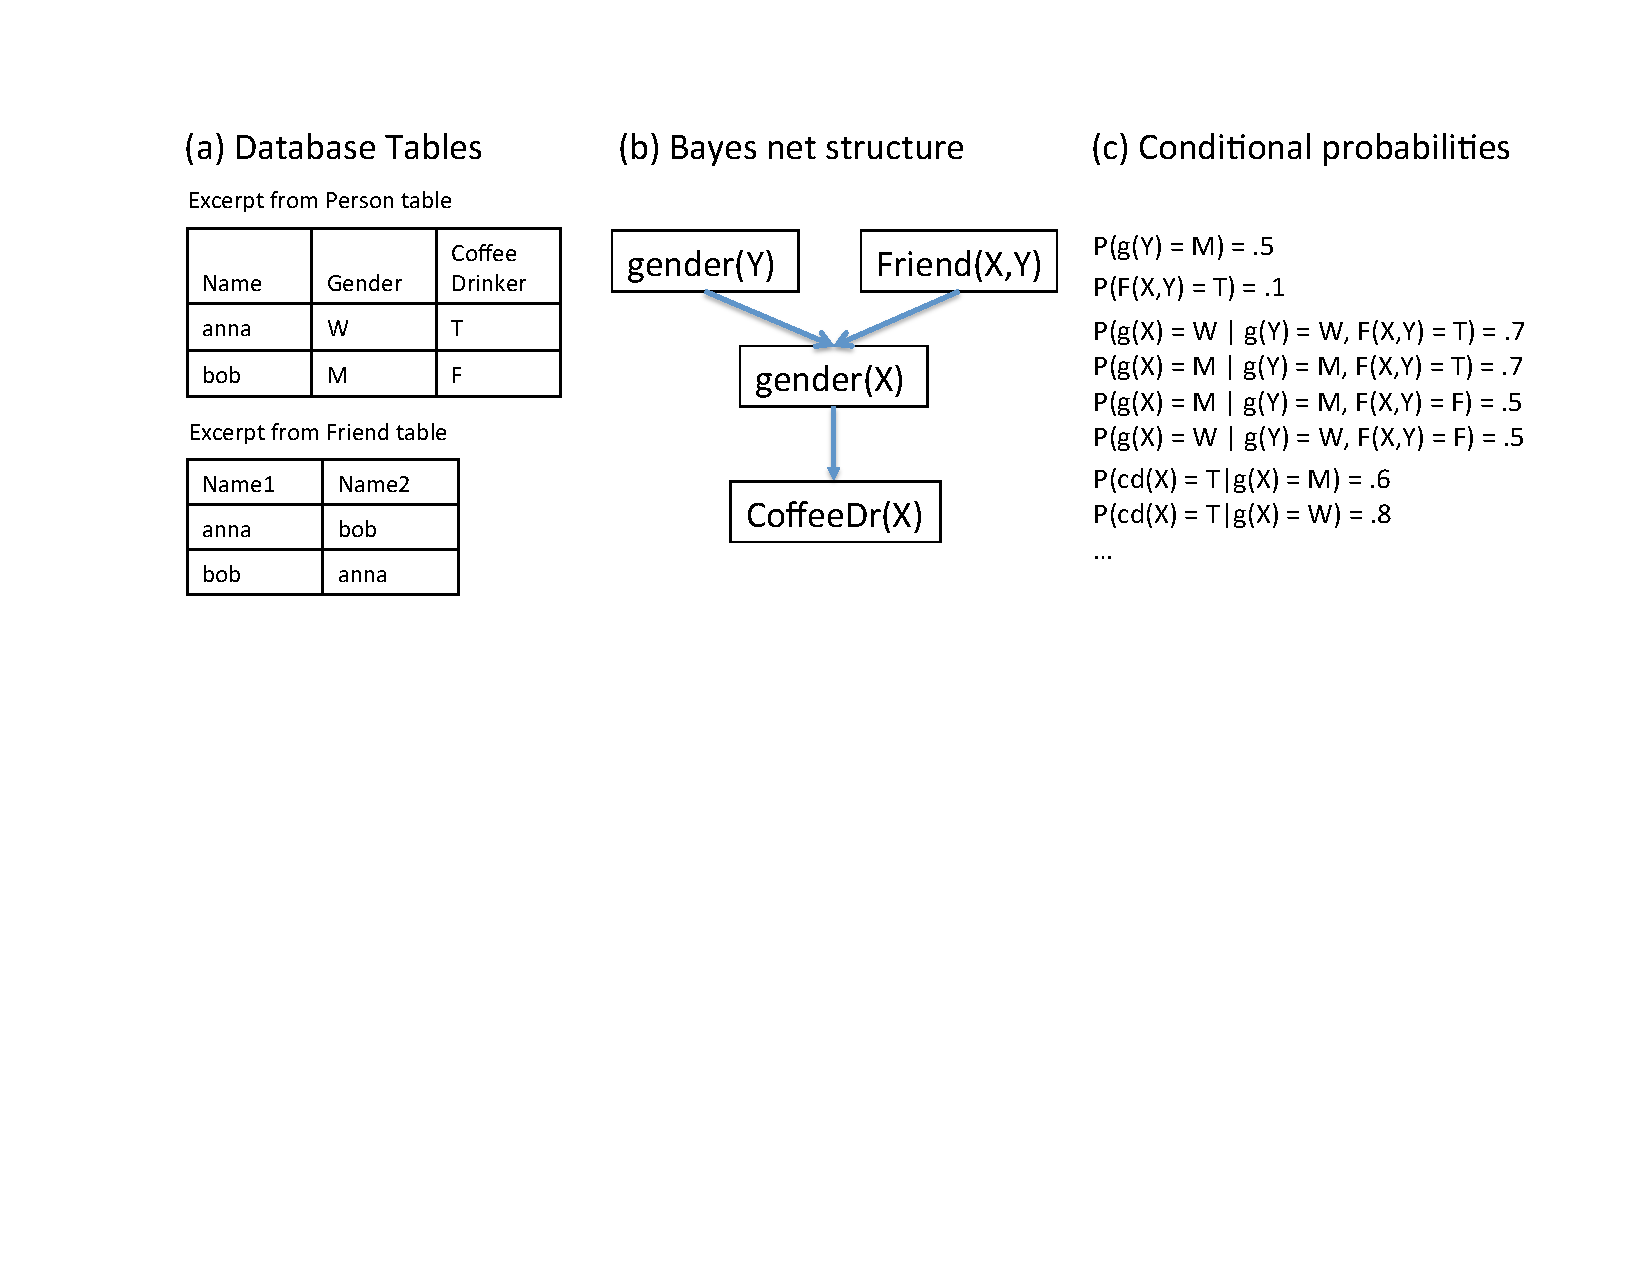
\includegraphics{figures/pbn-v3.pdf}
}
\caption{(a) A relational structure represented as tables. By convention, a pair not listed in the $\it{Friend}$ table are not friends. The $\it{Friend}$ relation is symmetric: $\it{Friend}(\X,\Y) = \it{Friend}(\Y,\X)$. Only part of the rows are shown. (b) A Bayes net structure for this database. $\it{Friend}(\X,\Y)$ is a relationship node, while the other three are attribute nodes. (c) The conditional probabilities for the Bayes net structure based upon the entries in the entire database.}
% with an autocorrelation on the attribute $\it{gender}$.
\label{fig:recurse}
\end{center}
\end{figure}

\subsection{Bayes Nets}

 A {\bf Bayes Net (BN)} is a directed acyclic graph (DAG) whose nodes comprise a set of random variables and conditional probability parameters.
For each assignment of values to the nodes, the joint probability 
is specified by the product of the conditional probabilities, $P(\it{child}|\it{parent\_values}$). 

A \textbf{Parametrized random variable} is of the form $\functor(\X_{1},\ldots,\X_{a})$, where the populations associated with the variables are of the appropriate type for the functor. 
%
A \textbf{Parametrized Bayes Net} (PBN) is a Bayes net whose nodes are parametrized random variables \cite{Poole2003}. In the remainder of this paper we follow \cite{Schulte2012} and use the terms $\textbf{functor random variable}$ and $\textbf{functor Bayes Net}$ instead (FBN), for the following reasons. (1) The name ``Parametrized'' denotes a semantics that views the Bayes net as a template for a ground graph structure. Our random selection semantics does not refer to a ground model.  (2) The usual statistical meaning of ``parametrized'' is that values have been assigned to the model parameters. We do not assume that such values have been assigned; learning them is a key topic of this paper. 

In our view, a Functor Bayes net is a type of Bayes net whose nodes are complex objects with an internal syntax derived from the relational structure. Where the distinction between BNs in general and FBNs is not important, we simply refer to FBNs as Bayes nets and to functor random variables as functor nodes or nodes. Figure~\ref{fig:recurse}(b)~shows an illustrative FBN. The next section presents a novel semantics of Functor Bayes nets as representing relational statistics.

\section{Random Selection Semantics for Bayes Nets}
\label{sec:class-level} 

%\paragraph{Functor Node Interpretation.}
%The random selection semantics views first-order/population variables $\X_{1},\X_{2}, \ldots, \X_{k}$ as independent random variables that each sample an individual from the appropriate population \cite{Halpern90,Bacchus90}. Then a functor of the form $\functor(\X_{1},\X_{2}, \ldots, \X_{k})$ represents a function of a random $k$-tuple. Since a {\em function of a random variable is itself a random variable}, this means that {\em we can view functor nodes as random variables in their own right, without grounding the variables first}. 

We provide a semantics that views a functor Bayes net as a representation of a joint probability distribution over its nodes \cite[Sec.14.2]{Russell2010}. The semantics is for nodes that refer to population variables, rather than for ground nodes that refer to individuals as in Poole's original paper \cite{Poole2003}. Such a nonground node can be given a probabilistic interpretation in terms of {\em random selections}. 

%\paragraph{Random Selection Semantics for Nodes With Population Variables.}

Consider first a node with a single population variable, e.g., $\it{gender}(\X)$. We view $\X$ as a random variable that selects a member $x$ from its population according to a uniform population distribution $P(\X = \x)$. The functor $\it{gender}$ then represents {\em a function of a random variable}, and hence is itself a random variable. Figure~\ref{fig:random-vars} illustrates this interpretation. 

\begin{figure}[t] %  figure placement: here, top, bottom, or page
   \centering
   \resizebox{1\textwidth}{!}{
   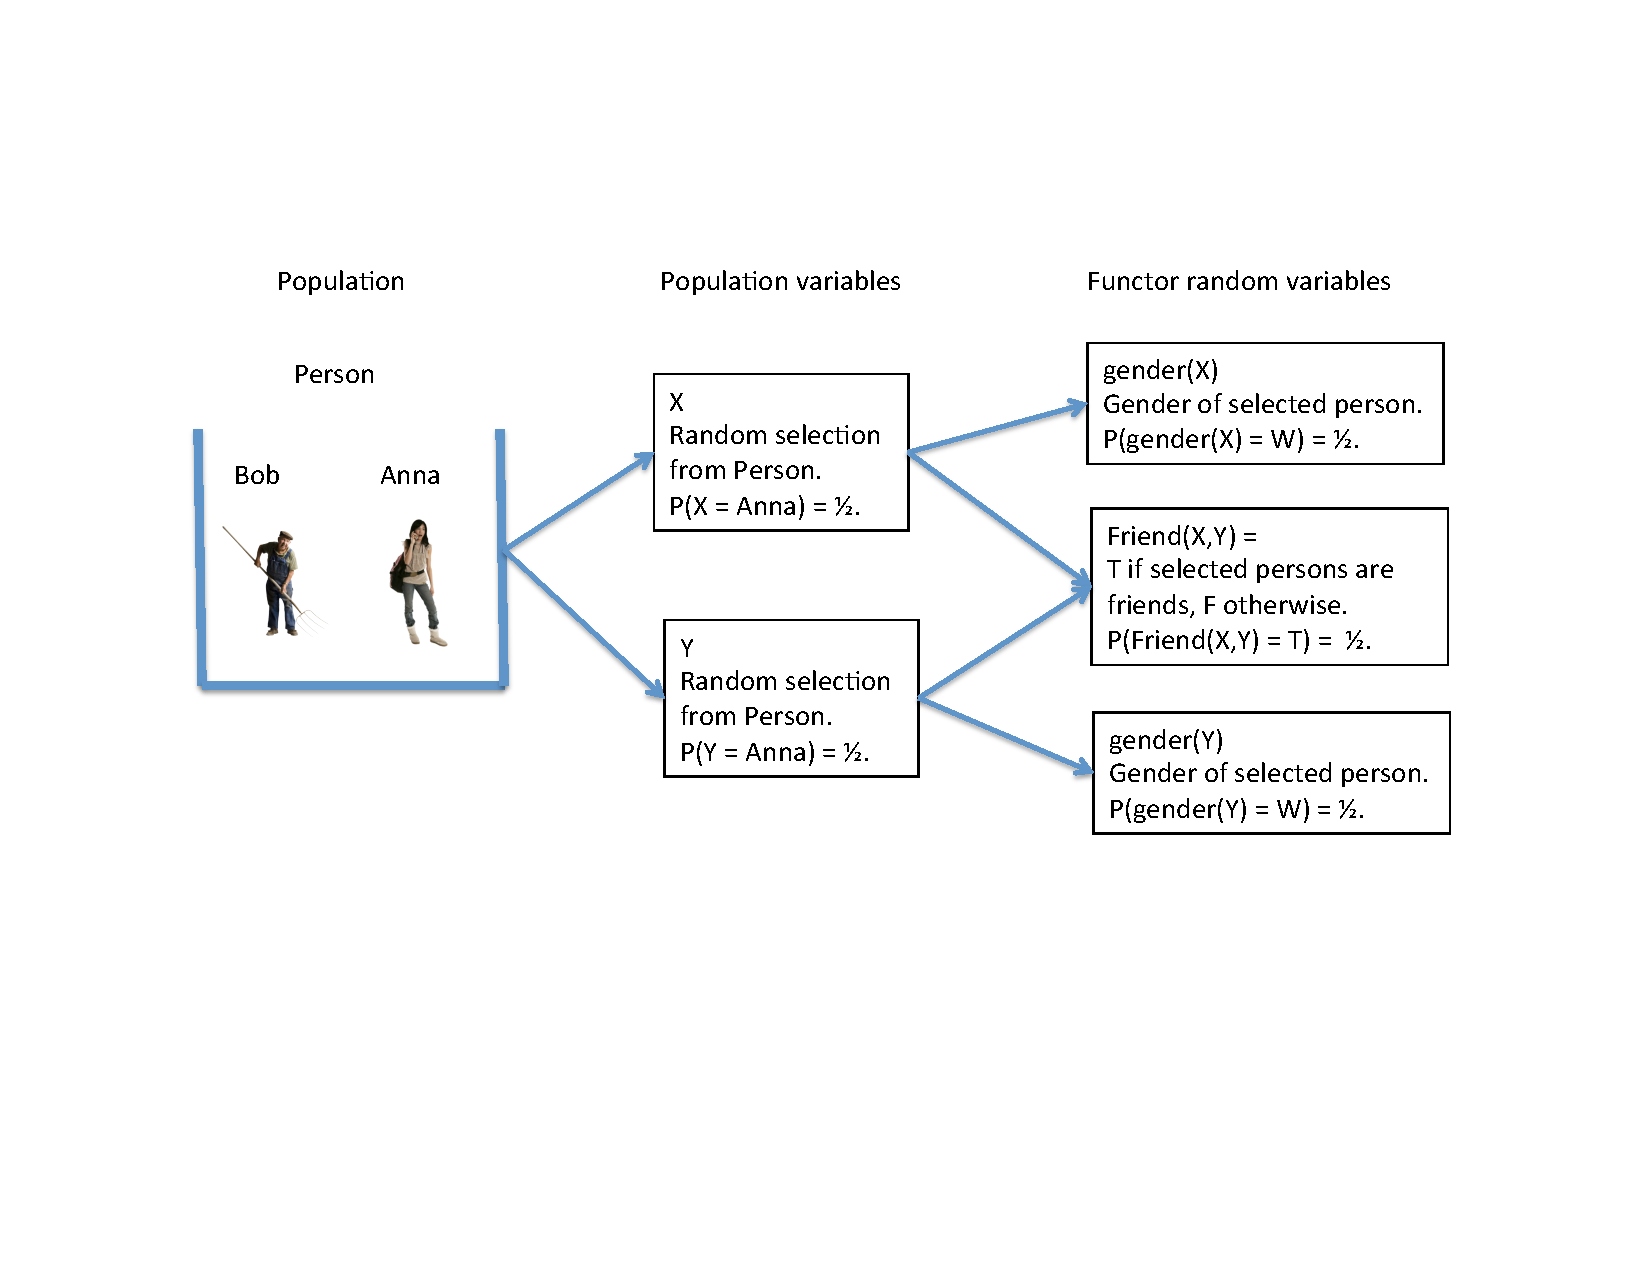
\includegraphics{figures/random-vars-v2.pdf} 
 }
\caption{Viewing population variables as random selections from the associated population, the  nodes represent functions of random variables, hence are themselves random variables. Probabilities are computed assuming the relations in Fig.~\ref{fig:recurse}~(a) are complete (the database only describes Bob and Anna). 
}
\label{fig:random-vars}
\end{figure}


In the case of a functor with several population variables $\functor(\X_{1},\ldots,\X_{a})$, we view each population variable as representing an independent selection from its associated population (thus variables for the same population represent i.i.d. selections). This defines a distribution over $a$-tuples of individuals from the appropriate population. Again, {\em any functor $\functor(\X_{1},\ldots,\X_{a})$ then defines a function of a random variable}, and hence is itself a random variable. Figure~\ref{fig:random-vars} illustrates the random selection interpretation for the functor $\it{Friend}(\X,\Y)$. 
%
As the random selection semantics is a key concept in this paper, we discuss two interpretations.

{\em Random Individuals.} Under random selection semantics, probability formulas can be interpreted as describing the properties of {\em random individuals.} For example, the formula $P(\it{gender}(\X) = M) = 50\%$ can be interpreted as ``the probability is 50\% that a randomly selected person is a man''. A related  interpretation that is often helpful is in terms of typical individuals \cite{Halpern90}; for instance, we may read the formula $P(\it{Flies}(\B) = \true) = 90\%$ as ``the probability that a typical bird flies is 90\%''. 

{\em Class-level Probabilities.} Random selection formulas can also be read as describing the distribution of properties in {\em classes of individuals}. Thus we can read $P(\it{gender}(\X) = M) = 50\%$ as ``the percentage of persons that are men is 50\%''. Similarly, we may read the formula $P(\it{Flies}(\B) = \true) = 90\%$ as ``the percentage of birds that fly is 90\%''. We therefore refer to probabilities defined by random selection as \textbf{class-level probabilities}. 

\paragraph{Random Selection Semantics for Bayes Nets.}
Random selection semantics can be applied to view Bayes nets as representing class-level probabilities, without reference to a ground model.
Via the standard product formula, a Bayes net $\B$ entails a probability value $\P_{\B}$ for each joint assignment of values to its  node. These are probability assignments that refer to population variables rather than individuals.
For example, the Bayes net structure of Figure~\ref{fig:recurse}~(b) entails joint probabilities of the form $$P_{\B}(g(\Y)=v_{1}, F(\X,\Y)=v_{2}, \g(\X) = v_{3}, CDr(\X)=v_{4}),$$ where we have used the obvious abbreviations for functors, and each $\v_{i}$ is a constant from the appropriate range. For example,  the conditional probabilities given in Figure~\ref{fig:recurse}(c) entail the joint probability

\begin{equation}\label{eq:statement}
\textstyle P_{\B}(g(\X) = W, g(\Y)=W, F(\X,\Y)=T, CDr(\X)=T) = .028.  %.5 \times .7 \times .1 \times .8 \approx 0.03.
\end{equation}

The random selection semantics for the nodes provides an interpretation of these joint probabilities. 
%As shown in Figure~\ref{fig:random-vars}, if we view each population variable as a random selection from its domain, then each functor expression associated with a node is a function of one or more random variables, and hence itself a random variable. The Bayes net therefore represents a joint distribution over random variables as usual. The extension from the nonrelational setting is simply that a random variable in the model is now a complex object with internal syntactic structure, rather than a simple object.  The random selection semantics provides a meaning for these structured random variables. 
For example, 
%using the obvious abbreviations for the BN of Figure~\ref{fig:recurse}, 
the joint probability~\eqref{eq:statement} can be read as ``if we randomly select two persons $\X$ and $\Y$, the chance is 2.8\% that they are both women, they are friends, and the first woman drinks coffee''.  

Since the random selection semantics is not defined in terms of a ground model, it can be applied even in the presence of cyclic dependencies in the data. For instance, grounding the Bayes net of Figure~\ref{fig:recurse} shows a cyclic dependency between the genders of different users. The random selection semantics still applies, as shown in our examples, since it concerns class-level dependencies. The BN of Figure~\ref{fig:recurse} illustrates that {\em the dependency structure among class-level random variables can be acyclic even when the dependency structure among ground instances is not}.

In logic, the term ``semantics'' is used in a different sense than in the context of statistical models, to refer to truth conditions for logical sentences \cite[Ch.7.4.2]{Russell2010}. In Section~\ref{sec:probability-logic}, we show that the random selection semantics for Bayes nets that we have presented is in agreement with Halpern's truth-conditional type 1 semantics for probabilistic logic. We next turn to learning and describe a method for learning Bayes net parameters that represent class-level probabilities. 

%We will describe the relationship of this semantics to probability logic in Section~\ref{sec:probability-logic}.

%
%%In Halpern's terminology, a Bayes net provides a compact representation of statistical assertions in a knowledge base \cite{Halpern2006}. 
%Using the axioms of probability calculus, we can derive further probability statements over the functor nodes, such as marginal and conditional probabilities. For instance, we have \\$P_{B}(\G(\X) = W|\G(\Y) = W) \equiv P_{B}(\G(\X) = W,\G(\Y) = W)/P_{B}(\G(\Y)=W)$.
%Random selection provides an interpretation for such probability statements. For instance, the meaning of Equation~\ref{eq:statement} is ``if we randomly select two users $\X$ and $\Y$, there is a 6\% chance that they are friends, both are women, and one is a coffee drinker''. Halpern develops this interpretation as a formal semantics for first-order formulas that state probability assignments \cite{Halpern90}.
%
%\paragraph{Database Queries and the Database Distribution.} 
%For each joint value assignment to nodes in a Bayes net there is a natural concept of the frequency with which this assignment holds in a given input database. The database frequency is the basis of the parameter learning algorithm we present below. It is connected to the cardinality of database queries, which is the basis for using Bayes net for selectivity estimation \cite{Getoor2001}. Consider a database query expressed in a {\em logical query language}, such as the domain relational calculus (DRC) \cite{Ullman1982}. An example would be 
%
%\begin{equation} \label{eq:query}
%\{\langle\X,\Y \rangle | G(\Y)=M, F(\X,\Y)=T, \G(\X) = W, CDr(\X)=T\}
%\end{equation}
%
%where $\X,\Y$ are the {\em query variables} that occur free (unquantified) in the query formula.
%The query returns the set of all people pairs $\langle \x,\y \rangle$ that satisfy the query formula. Logical queries are very powerful: a fundamental result in database theory states that a subset of DRC queries known as safe queries has expressive power equivalent to relational algebra \cite{Ullman1982}. The cardinality of a query is the number of tuples returned; the cardinality of Query~\ref{eq:query} applied to the data of Figure~\ref{fig:recurse} is 1. Assuming an assignment of types to the query variables, the largest possible query result is the cross-product of the type domains. Thus the \textbf{database frequency} of a query is the cardinality of the query, divided by the product of the domain sizes for the query variables. The database frequency for Query~\ref{eq:query} in the database of Figure~\ref{fig:recurse} is 
%
%\begin{equation} \label{eq:query}
%P_{\D}(G(\Y)=M, F(\X,\Y)=T, \G(\X) = W, CDr(\X)=T) = \frac{1}{2 \cdot 2}.
%\end{equation}
%We refer to $P_{\D}$ as the \textbf{database distribution} over functor node assignments. Assuming knowledge of the type domain associated with the query variables, the database frequency $P_{\D}$ immediately gives an estimate of the query cardinality.
%It is easy to see that the database distribution coincides with the random selection semantics when the random selection is uniform over the individuals listed for a given type in the database. 

\section{Parameter Learning For Class-Level Probabilities} \label{sec:learning}

In a nonrelational learning setting, it is common to view a data table as representing information about individuals in a finite subset drawn from a large, possibly infinite population. In relational learning, we view a \textbf{database} $\D$ as representing a finite substructure of a large, possibly infinite relational structure. 
%We denote the source database by $\D$. 
We make the standard assumption that the database is complete \cite{Domingos2009,Khot2011}: For each individual (node) observed, the database lists its attributes, and for each pair of observed individuals (nodes), the database specifies which links hold between them. Note that completeness is a statement about the information about individuals in the database. A complete database may contain only a subset of the individuals in the population about which we wish to make inferences. %We discuss learning with incomplete relational data in Section~\ref{sec:incomplete}.

%A data generation method that supports the complete-data assumption is subgraph sampling, which has been studied by network statisticians for decades \cite{Frank1977,Khosravi2010}. Subgraph sampling selects entities of each type uniformly at random, and checks for each pair of observed individuals which links hold between them. The subgraph method satisfies an ergodic law of large numbers in the sense that as the sample size increases, the substructure relational frequencies approach the complete-structure relational frequencies. 
%While our experiments use subgraph sampling, the general theory and algorithms that we develop in this paper do not depend on the particular data generation method used. However, applying them correctly to a data set may require consideration of how the data were generated, for example by smoothing, or correcting for selection bias.

A fundamental question for statistical model selection is how to measure the fit of the model. That is, we must specify a likelihood function $P_{\B}(\D)$ for a given database. 
%A natural candidate for the likelihood function is the distribution $\mu_{\B}$ defined by the template semantics described in Section~\ref{sec:instance-level}. However, this likelihood function is intractable, and in the presence of cyclic dependencies, it is not well defined. Instead, 
The random selection semantics can be used to define a tractable {\em pseudo-likelihood}~\cite{Schulte2011}: The pseudo log-likelihood is the expected log-probability assigned by the Bayes net to the links and attributes for a {\em random instantiation} of the population variables. This is defined by the following procedure.

\begin{enumerate}
%\item Let $\X_{1},\ldots,\X_{k}$ be a list of {\em all} 1st-order variables that occur in the functor nodes of the parametrized Bayes net $\B$.
\item Randomly select a grounding for {\em all} population variables that occur in the Bayes net. The result is a ground graph with as many nodes as the original.
%an instance (constant) $\value_{i}$ from the population of variable $\X_{i}$, for each $i=1,\ldots,k$.
%\item  Replace each variable in $\B$ with the corresponding instance so each vnode in $\B$ becomes a gnode. 
\item Look up the value assigned to each ground node in the database.
Compute the log-likelihood of this joint assignment using the usual product formula; this defines a log-likelihood for this random instantiation. 
\item The expected value of this log-likelihood---the mean over all instantiations---is the {\em pseudo log-likelihood}  of the database given the Bayes net. 
\end{enumerate}

\newcommand{\pseudologp}{-3.42}


\begin{table}[tb]
\caption{An example computation of the pseudo-likelihood for the database  and the Bayes net of Figure~\ref{fig:recurse}~(b). Columns for functors include the grounded value and its conditional probability.  The dotted row indicates entries for combinations including the other instances of {\em Person}. The pseudo log-likelihood is the mean of the ln~$p$ column.}
%The pseudo log-likelihood is \pseudologp{}, the average of the ln~$p$ column. }
\begin{center}
%\resizebox{1\textwidth}{!}
\begin{tabular}{|c|c|c|c|c|c||c|c|}
\hline
X & Y & g(Y) & F(X,Y) & g(X) & cd(X) & Joint $p$ & ln~$p$ \\ \hline
anna & anna & W (0.5) & F (0.9) & W (0.5) & T (0.8) & 0.180 & -1.71\\
anna & bob & M (0.5) & T (0.1) & W (0.3) & T (0.8) & 0.012 & -4.42\\
bob & anna & W (0.5) & T (0.1) & M (0.3) & F (0.4) & 0.006 & -5.12\\
bob & bob & M (0.5) & F (0.9) & M (0.5) & F (0.4) & 0.090 & -2.41\\
\ldots & \ldots & \ldots & \ldots & \ldots & \ldots & \ldots & \ldots\\
\hline
\end{tabular}

\end{center}
\label{table:entity-join}
\end{table}

\noindent Table~\ref{table:entity-join} shows an example computation of the pseudo likelihood.
%
The pseudo likelihood matches the random selection semantics that we have proposed for class-level Bayes nets. It has several attractive theoretical properties \cite{Schulte2011}. (1) Because it does not make reference to a single ground model, the measure is well defined even in the presence of cyclic dependencies in the data. For instance, grounding the Bayes net of Figure~\ref{fig:recurse} shows a cyclic dependency between the genders of different users. Nonetheless a pseudo-likelihood value can be computed as in Table~\ref{table:entity-join}. The pseudo-likelihood can be used to effectively learn cyclic or recursive dependencies \cite{Schulte2012}. (2) It is closely related to relational pseudo-likelihood measures proposed for other graphical models (e.g., Markov random fields). (3) It is invariant under equivalence transformations of the logical predicates (database normalization). (4) For a fixed database $\D$ and Bayes net structure, {\em the parameter values that maximize the pseudo-likelihood are the conditional empirical frequencies observed in the database} \cite[Prop.3.1]{Schulte2011}. We refer to these frequencies as the \textbf{database probabilities.} This result is exactly analogous to  maximum likelihood estimation for i.i.d. data, where the empirical frequencies in an i.i.d. sample maximize the  model likelihood.

The database probability distribution $P_{\D}$ of a node assignment is the number of instantiations of the population variables in the functor nodes that satisfy the assignment in the database, divided by the number of all possible instantiations. The formal definition is~\cite{Chiang2012}:

\begin{itemize}
\item Let $\f_{1} = \nodevalue_{1}, \ldots, \f_{n} = \nodevalue_{n}$ be an assignment of appropriate values to $n$ nodes. 
\item Let $\X_{1},\ldots,\X_{\ell}$ be the population variables that appear in the nodes, with associated population sizes $|\population_{1}|, \ldots, |\population_{\ell}|$.
\item Let $\grounds_{\D}(\f_{1} = \nodevalue_{1}, \ldots, \f_{n} = \nodevalue_{n})$ be the number of instantiations or groundings of the population variables that satisfy the assigned values in $\D$.
\item Then the database probability of the value assignment is given by

$$P_{\D}(\f_{1} = \nodevalue_{1}, \ldots, \f_{n} = \nodevalue_{n}) = \frac{\grounds_{\D}(\f_{1} = \nodevalue_{1}, \ldots, \f_{n} = \nodevalue_{n})}{|\population_{1}| \times \cdots \times |\population_{\ell}|}.$$
\end{itemize}

\paragraph{Example.} Following Figure~\ref{fig:recurse}(b), where the complete person population is $\{anna$, $bob\}$, we have 
%%\begin{scriptsize}

$$P_{\D}(\it{gender}(\X) = M) = 1/2$$ and

$$P_{\D}(\it{Friend}(X,Y) = \true, \it{gender}(\X) = M, \it{gender}(\Y) = W) = 1/4.$$ 
%%\end{scriptsize}
%
%The database distribution can be viewed as a special case of the random selection semantics as follows: Take the database as a relational structure, identify each population with the set of individuals of the appropriate type listed in the database, and take the uniform distribution over this set as the population distribution.
%
In the next section we consider how
to compute database probabilities.


\section{Computing Relational Statistics} \label{sec:mobius}

In this section we describe algorithms for computing  probability estimates for the parameters $P_{\D}(\it{child}\_value,\it{parent}\_\it{values})$ in a functor Bayes net. The parameters can be estimated independently for each child node. We refer to a joint specification of values $(\it{child}\_value,\it{parent}\_\it{values})$ as a \textbf{family state}. Consider a child node specifying a relationship $\R_{1}$ whose parents comprise relationship nodes $R_{2},\ldots,R_{m}$, and attribute nodes $\functor_{1},\ldots,\functor_{j}$. The algorithms below can be applied in the same way in the case where the child node is an attribute node. The number of family states $r$ is the cardinality of the Cartesian product of the ranges for every node in the family.
 The Bayes net parameters are $r$ conditional probabilities of the form (we separate relationships from attributes by a semicolon)
\begin{equation} \label{eq:cond-prob}
P(\R_{1} = b_{1}| R_{2} = b_{2},\ldots, R_{m} = b_{m}; \functor_{1} = v_{1},\ldots,\functor_{j} = v_{j}),
\end{equation}
where the $b_{i}$ values are Boolean and each $v_{i}$ is from the domain of $\functor_{i}$. 
Figure~\ref{fig:example}~(Top) provides an example with $\R_{1} = \it{Follows}(\X,\Y)$, $\R_{2} = \it{Friend}(\X,\Y)$, and $\functor_{1} = \it{gender}(\X)$. In this example, all nodes are binary, so the CP-table requires the specification of $r= 2 \times 2 \times 2 = 8$ values.\footnote{Although only 4 of these values are independent, we take the number of parameters to be $r = 8$ for simplicity of exposition of the inverse Moebius transform in the next section.}

\begin{figure}[tb]
\begin{center}
\resizebox{1\textwidth}{!}{
%%!%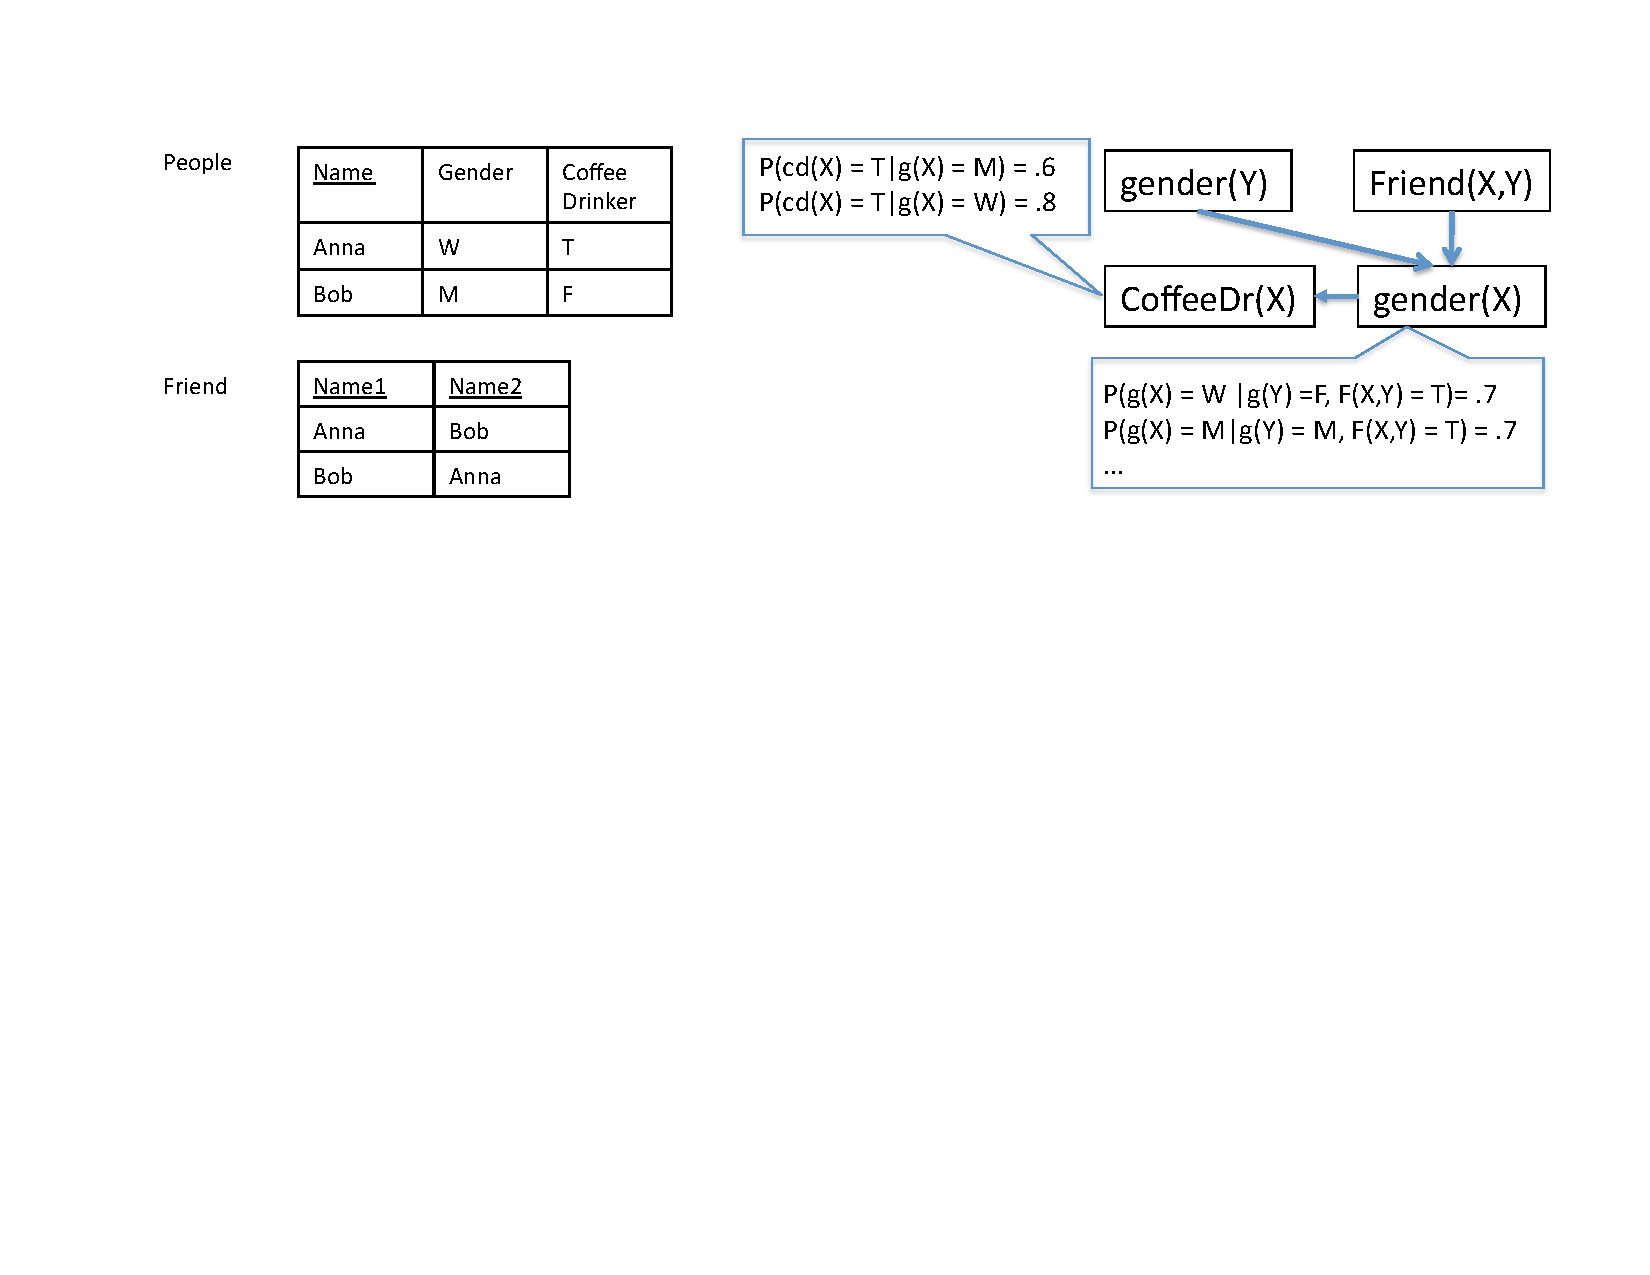
\includegraphics[width=1\textwidth]{pbn}
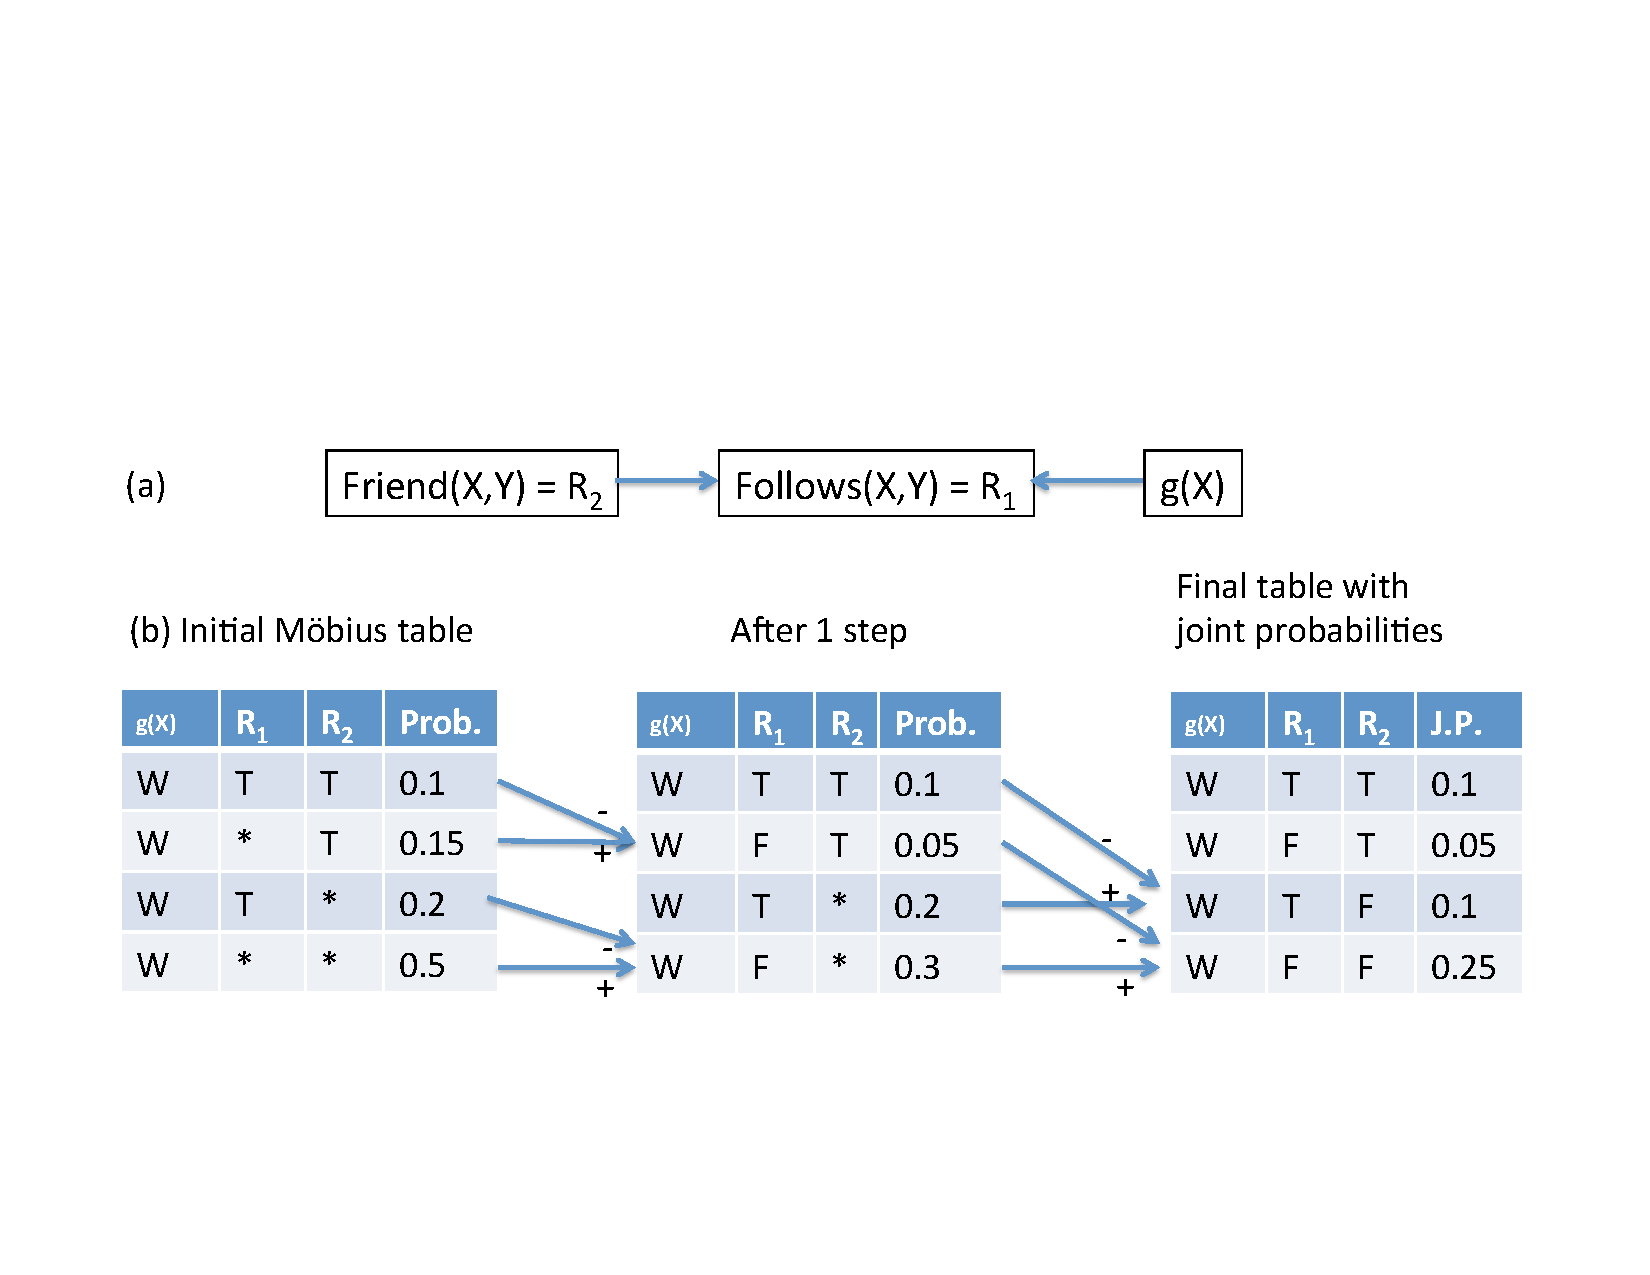
\includegraphics{figures/mobius-v2.pdf}
}
\caption{(a) A Bayes net with two relationship nodes. (b) An illustrative trace of the inverse M\"obius transform (see text). 
\label{fig:example}}
\end{center}
\end{figure}


Conditional probabilities can be easily estimated from the {\em sufficient statistics}, which are the database probabilities for a family state:

\begin{equation} \label{eq:joint-prob}
P_{\D}(\R_{1} = b_{1}, R_{2} = b_{2},\ldots, R_{m} = b_{m}; \functor_{1} = v_{1},\ldots,\functor_{j} = v_{j}).
\end{equation}

\noindent For the rest of this section, we focus on computing these joint probabilities. So long as a database probability involves only positive relationships,
%formula only contains positive relationships, 
the computation is straightforward. 
For example, in 
$P_{\D}(\it{gender}(\X) = M, \it{Friend}(\X,\Y) = \true)$, the value  $\grounds_{\D}(\it{gender}(\X) = M, \it{Friend}(\X,\Y) = \true)$, the count of friendship pairs $(x,y)$ where $x$ is male and the
{\em Friend} relationship is true, can be computed by regular table joins or optimized virtual joins~\cite{Yin2004}. 

Computing joint probabilities for a family containing one or more negative relationships is harder. A naive approach would explicitly construct new data tables that enumerate tuples of objects that are {\em not} related. 
%and then apply existing counting methods to the new tables. 
However, the number of unrelated tuples is too large to make this scalable (think about the number of user pairs who are {\em not} friends on Facebook). 
%A numerical example will illustrate why this is not feasible. Consider a university database with 20,000 Students, 1,000 Courses and 2,000 TAs. If each student is registered in 10 courses, the size of a $\it{Registered}$ table is 200,000. So the number of complementary student-course pairs is $2 \times 10^{7}-2 \times 10^{5}$, which is too big for most database systems. 
%If we consider joins, complemented tables are even more difficult to deal with: suppose that each course has at most 3 TAs. Then  the number of satisfying instantiations of a positive relationship only formula such as $\it{Registered}(\S,\C) = \true,\it{TA}(\T,\C) = \true)$ is less than $6 \times 10^{5}$, whereas with negations the number of instantiations of the expression $\it{Registered}(\S,\it{course}) = \false, \it{TA}(\T,\it{course}) = \false)$ is on the order of $4 \times 10^{10}$. 
%\subsection{The M\"obius parametrization.} 
%To compute frequencies involving negated relationships, we would like to use the optimized algorithms for table join frequencies as an oracle/black box. 
%Can we instead reduce the computation of sufficient statistics that involve negated relationships to the computation of sufficient statistics that involve existing (positive) relationships only? 
In their work on learning Probabilistic Relational Models with existence  uncertainty, Getoor et al. provided a ``1-minus trick'' for the special case of estimating a conditional probability with only a single negated relationship \cite[Sec.5.8.4.2]{Getoor2007c}. They did not treat parameter learning with multiple negated relationships.
%this method does not extend to multiple negated relationships.

\subsection{Statistics With Multiple Negated Relationships: The Fast M\"obius Transform} 

%The classic 
%M\"obius parametrization for binary random variables provides an affirmative answer \cite[p.239]{Lauritzen1996}. Consider a set $b_{1},\ldots,b_{m}$ of binary variables, where all marginal probabilities are available that involve only positive values. Thus we have available probabilities such as $P(b_{1}= 1)$; $P(b_{1} = 1, b_{2} = 1)$; $P(b_{1} = 1, b_{3} = 1, b_{k} = 1);$ etc. 
%%For conciseness, we write $P(A = \bs{1})$ for the marginal probability where the values of all variables $i \in A, i = 1, \ldots, m$ are specified to be 1. Thus the probabilities above are written as $$P(\{1\}= \bs{1}), P(\{1,2\}= \bs{1}), P(\{1,3,k\}= \bs{1}).$$
%These joint probabilities %with positive values only 
%are the \textbf{M\"obius parameters} of the joint distribution. The M\"obius inversion theorem entails that {\em all} joint probabilities, involving any number of 0 values, can be computed as an alternating sum of the M\"obius parameters. 
%The computation uses an alternating sum as follows. Extending the previous notation, let us write $P(A = \bs{1}, \bar{A} = \bs{0})$ for the joint probability where the variables in set $A$ are assigned value 1, and the remaining variables are assigned 0. Then the M\"obius parametrization theorem states that
%
%\begin{equation} \label{theo:moebius}
%P(A = \bs{1}, \bar{A} = \bs{0})  = \sum_{B \supseteq A} -1^{|B-A|} P(B = \bs{1})
%\end{equation}
%where $P(\emptyset = \bs{1}) := 1$ by definition.
%{\em Examples.} Suppose that we have only a single random variable $b_{1} = b_{k}$. Then $P(b_{1} = 0) = P(\emptyset = 1)$ in the notation above. Therefore the parametrization implies that
%
%$$
%P(b_{1} = 0) = -1^{0} P(\emptyset = 1) + 1^|\emptyset - \{1\} P(b_{1} = 1) = 1- P(b_{1} = 1).
%$$
%
%For another example consider two binary random variables $b_{1}, b_{2} = b_{k}$. Then 
%
%$$
%P(b_{1} =0, b_{2} = 0) = 1 - P(b_{1} = 1) - P(b_{2} = 1) + P(b_{1} = 1, P(b_{2} = 1).
%$$
%
%We can apply this result for MPLE as follows. Consider a FBN family containing $m$ relationship nodes. We wish to compute frequencies of the joint family assignments, %$\family_{ijk}$, 
%from which conditional probabilities are easily derived. The M\"obius inversion theorem entails that each joint frequency {\em can be computed from joint frequencies that involve existing relationships only.} 
%
%{\em Example.} Suppose we wish to compute $P_{\D}(\it{intelligence}(\S) = 1, \it{Registered}(\S,\C) = \false, \it{RA}(\S,\P) = \false).$ Abbreviating $\it{intelligence}(\S) = 1$ as $I(S) = 1$, the 4 M\"obius parameters are $P_{\D}(I(S) = 1)$; $P_{\D}(I(S) = 1, \it{Reg}(\S,C) = \true)$; $P_{\D}(I(S) = 1, \it{RA}(\S,\P) = \true)$; and $P_{\D}(I(S) = 1, \it{Reg}(\S,C) = \true, \it{RA}(\S,\P) = \true)$. The M\"obius inversion theorem implies that the desired joint frequency can be computed as an alternating sum of these 4 values. 
%
%Since our goal is to compute {\em all} joint frequencies, it is inefficient to apply the M\"obius formula to each, because then many partial sums are computed repeatedly. 


% Equation~\eqref{theo:moebius} for computing sufficient statistics as follows. Consider a frequency of the form $P_{\D}(\set{C}, \set{R})$, where $\set{C}$ is an assignment of values to attributes and $\set{R}$ is an assignment of Boolean values to relationship functors. For a fixed attribute condition $\set{C}$, the sufficient statistic is just a function of binary relationship variables. Equation~\eqref{theo:moebius} shows that this frequency can be written as an alternating sum of frequencies of the form $P_{\D}(\set{C},\set{R'})$ where {\em $\set{R'}$ sets all relationship functors in the list to be true.} Since these frequencies involve no false relationships, they can be computed using standard table joins.
%
%For example, suppose we want to compute the frequency $P_{\D}(\it{Int}(\S) = 1, \it{Reg}(\S,C) = \false, \it{RA}(\S,\P) = F)$, with just one attribute in the attribute condition and two relationship functors each assigned the value false. The M\"obius theorem implies that this can be written as an alternating sum of the M\"obius parameters $P_{\D}(\it{Int}(\S) = 1)$; $P_{\D}(\it{Int}(\S) = 1, \it{Reg}(\S,C) = \true)$; $P_{\D}(\it{Int}(\S) = 1, \it{RA}(\S,\P) = \true)$; and $P_{\D}(\it{Int}(\S) = 1, \it{Reg}(\S,C) = \true, \it{RA}(\S,\P) = \true)$. Once we have computed all joint frequencies over the nodes in a family, the conditional probabilities for the child are easily computed by summation. 
%Next we discuss how to compute all joint family frequencies efficiently. 

%\subsection{The Fast M\"obius Transform} 
%Using Equation~\eqref{theo:moebius} for each joint probability is inefficient because many of the alternating partial sums are recomputed repeatedly. Kennes and Smets designed the \textbf{inverse M\"obius transform} as a highly efficient algorithm for discovering all joint probabilities from the M\"obius parameters\cite{Kennes1990}. 

The general case of multiple negative relationships can be efficiently computed using
the \textbf{fast inverse M\"obius transform} (IMT), or M\"obius transform for short. 
We compute the  joint probabilities \eqref{eq:joint-prob} for $r$ family states by first computing the $r$  M\"obius parameters of the joint distribution, then using the inverse M\"obius transform to transform the M\"obius parameters into the desired joint probabilities. Figure~\ref{fig:flow} provides an overview of the computation steps. Because the M\"obius parameters involve probabilities  for events with {\em positive relationships only}, they can be estimated directly from the data. 
We next define the M\"obius parameters, then explain the IMT.

\begin{figure}[t]
\begin{center}
\resizebox{1\textwidth}{!}{
%%!%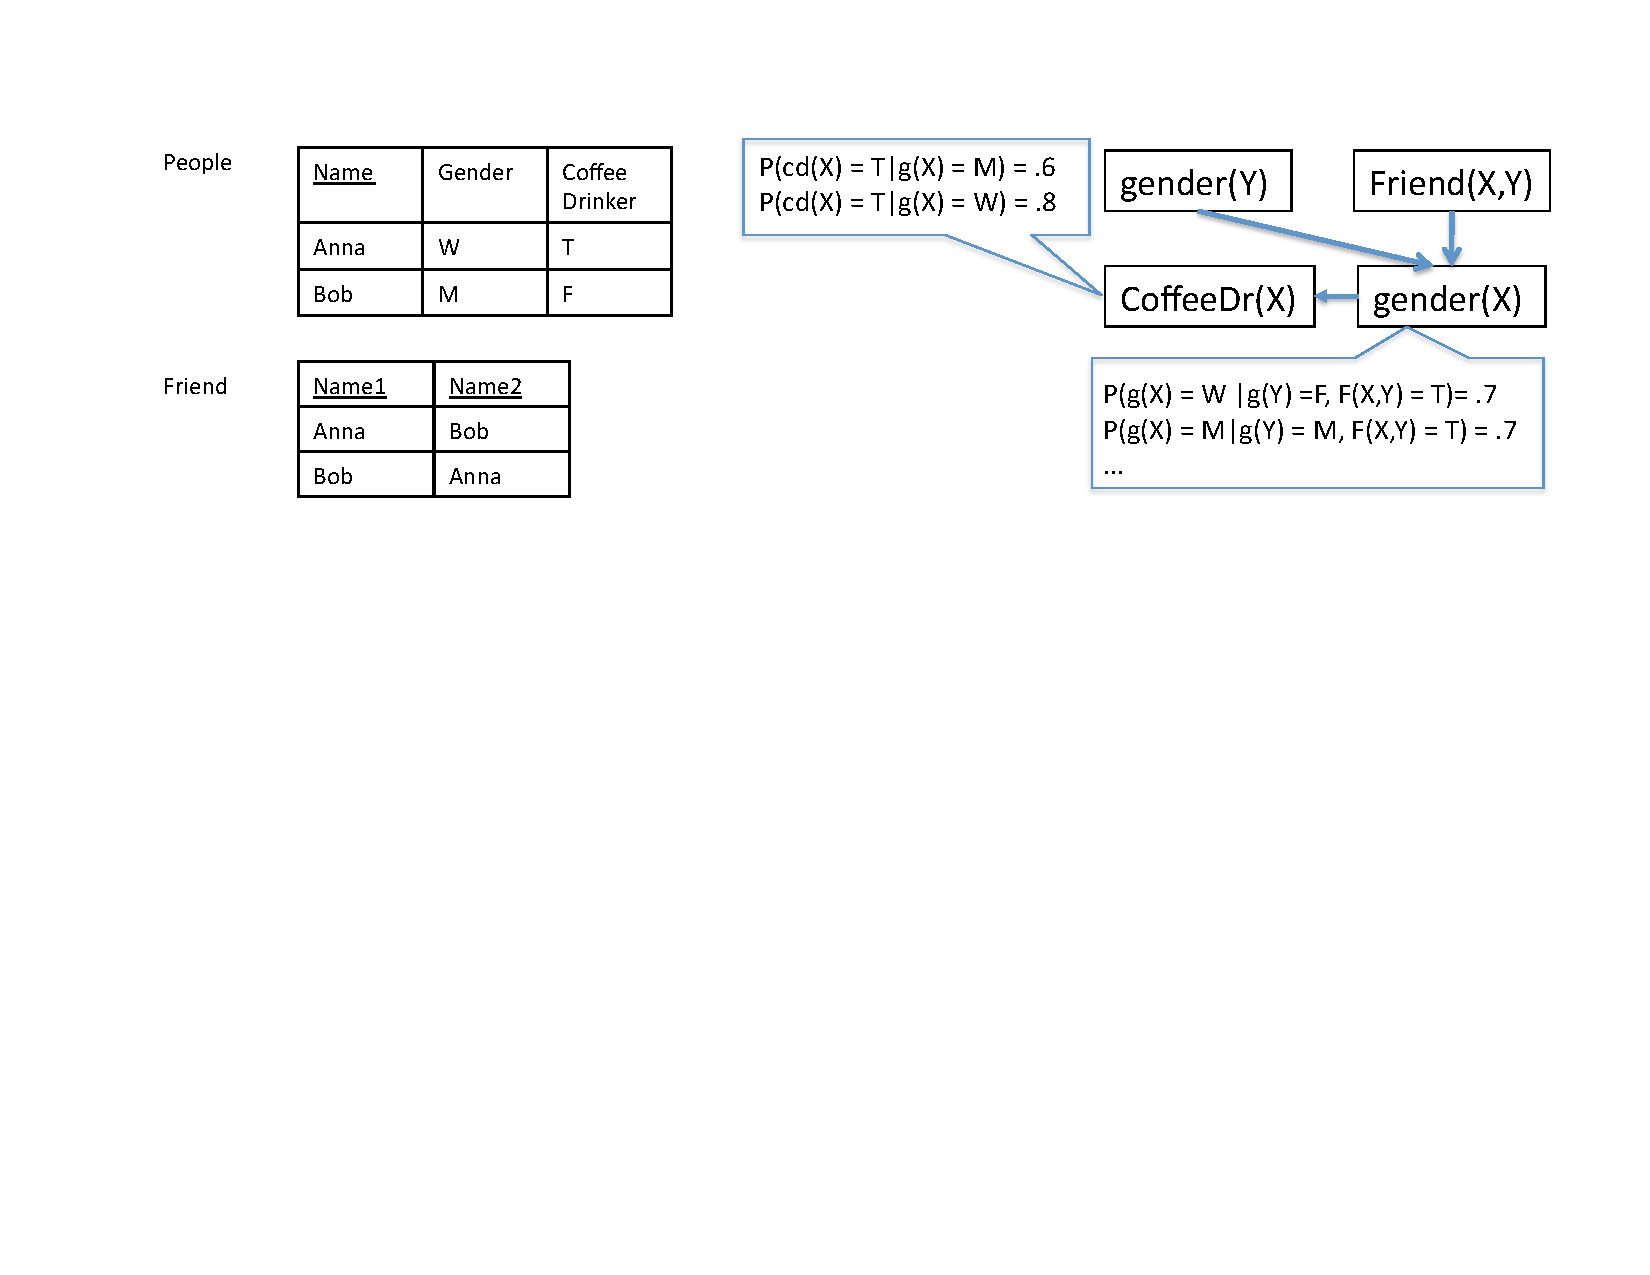
\includegraphics[width=1\textwidth]{pbn}
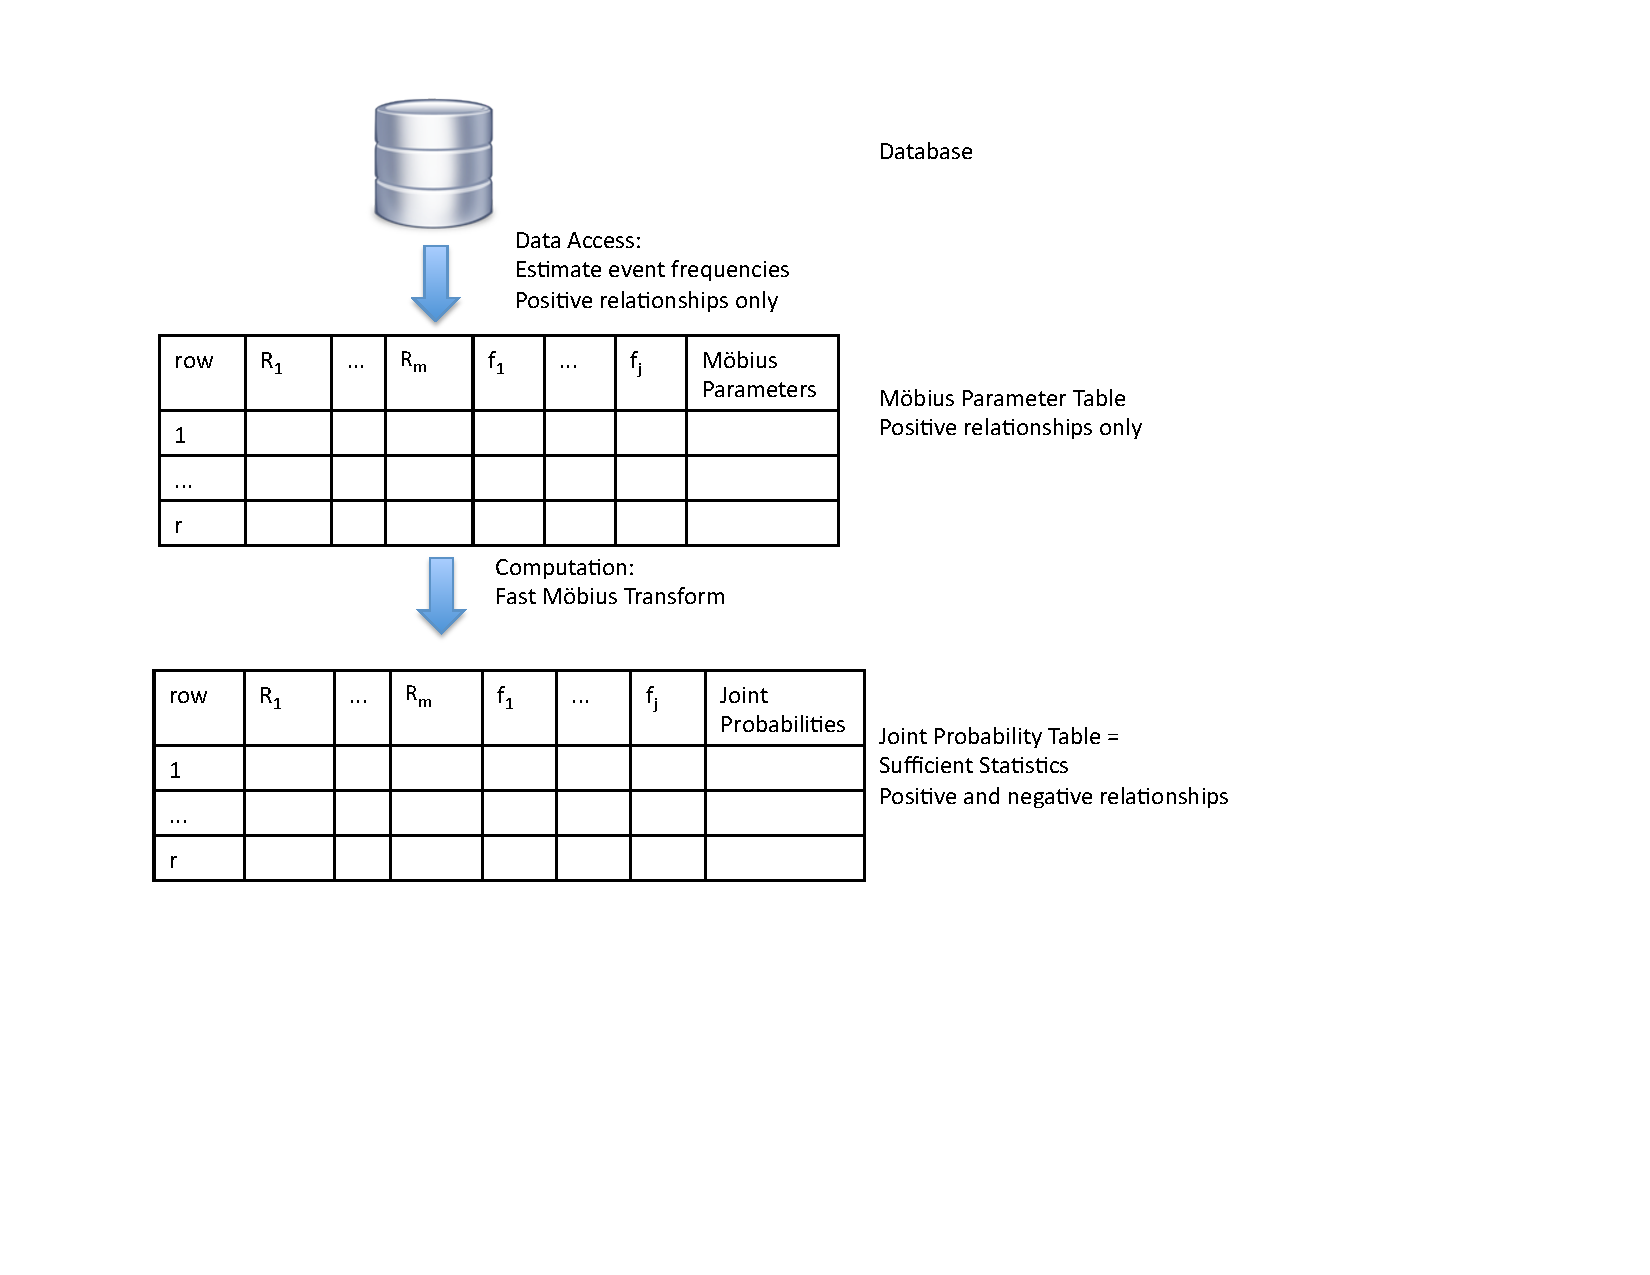
\includegraphics{figures/flow.pdf}
}
\caption{Computation of joint probabilities in a relational database. (1) Estimate M\"obius parameters using standard table join operations. (2) Transform the M\"obius parameters into joint probabilities. (3) Compute conditional probabilities from joint probabilities.
Only the first step involves data access.
\label{fig:flow}}
\end{center}
\end{figure}

%
%Our approach is to successively reduce the problem of estimating the $r$ conditional probabilities to estimating another set of $r$ probabilities, to the point where we need to estimate from the data only events that involve positive relationships. Figure~\ref{fig:flow} provides a overview of the reduction steps. 
%
%{\em Reduction 1} replaces the problem of computing the $r$ conditional probabilities ~\eqref{eq:cond-prob} by the problem of computing the $r$ {\em joint probabilities} of the form 
%
%\begin{equation} \label{eq:joint-prob}
%P(\R_{1} = b_{1}, R_{2} = b_{2},\ldots, R_{m} = b_{m}, \functor_{1} = v_{1},\ldots,\functor_{j} = v_{j}).
%\end{equation}
%
%The conditional probabilities are easily obtained from the joint probabilities via the identity
%
%$$P(\R_{1} = b_{1}|\parents) = \frac{P(\R_{1} = b_{1},\parents)}{P(\R_{1} = \true,\parents)+P(\R_{1} = \false,\parents)}.$$

%{\em Reduction 2} replaces the problem of computing the $r$ joint probabilities ~\eqref{eq:joint-prob} by the problem of computing the $r$  M\"obius parameters of the joint distribution. The reason for using the M\"obius parameters is that they involve probabilities  for events with {\em positive relationships only}. Hence they can be estimated using regular joins or optimized virtual joins ~\cite{Yin2004}.  
%
%The inverse M\"obius transform is an optimal algorithm for computing the joint probabilities from the M\"obius parameters. We explain the IMT later in this section. The last step is to estimate the M\"obius parameters directly from the data.
%
%We use
%%adapt the original lattice-structure formulation of IMT
%the transform to compute \textbf{joint probability tables} (JP-tables), CP-tables where the conditional probabilities are replaced by joint probabilities. 
%For simplicity, we explain the IMT for a fixed attribute conjunction $\literal$ and do not mention $\literal$ further in the description of the algorithm. 

Let $\mathbb{B} = \B_{1},\ldots,\B_{m}$ be a set of binary random variables with possible values 0 or 1, and $P$ be the joint distribution that specifies $2^{m}$ probabilities, one for each possible assignment of values to the $m$ binary variables. For any subset $\set{B} \subseteq \mathbb{B}$ of the variables, let $P(\set{B} = \set{1})$ denote the probability that the variables in $\set{B}$ are assigned the value 1, leaving the value of the other variables unspecified. The \textbf{M\"obius parameters} of the distribution $P$ are the values $P(\set{B} = \set{1})$ for all subsets $\set{B} \subseteq \mathbb{B}$\cite[Sec.3]{Drton08}.
There are $2^{m}$ M\"obius parameters for $m$ binary variables, with $0\leq P(\mathbb{B}=\set{1})\leq P(\set{B}=\set{1})\leq P(\emptyset=\set{1}) = 1$.

For a family state, if we fix the values $\v_{1},\ldots,\v_{j}$ of the attribute atoms, the sufficient statistics correspond to a joint distribution over $m$ Boolean relationship random variables:

$$P(\R_{1} = \cdot, R_{2} = \cdot,\ldots, R_{m} = \cdot; \functor_{1} = v_{1},\ldots,\functor_{j} = v_{j}).$$

\noindent We refer to the M\"obius parameters of this joint distribution as the \textbf{M\"obius parameters for the attribute values} $\v_{1},\ldots,\v_{j}$.

\paragraph{Example.} For the Bayes net of Figure~\ref{fig:example}~(Top), fix the attribute condition $\it{gender}(\X) = W$. The four M\"obius parameters for this attribute condition are
 %$P(\it{gender}(\X) = W)$, 
%$P(\it{Friend}(\X,\Y) = \true; \it{gender}(\X) = W)$, 
%$P(\it{gender}(\X) = W,\it{Follows}(\X,\Y) = \true; \it{gender}(\X) = W)$, 
%$P(\it{gender}(\X) = W,\it{Friend}(\X,\Y) = \true, \it{Follows}(\X,\Y) = \true; \it{gender}(\X) = W)$.
%\marginpar{do these need to be put in an equation array?}
%\begin{eqnarray*}
\begin{flalign*}
&P(\it{gender}(\X) = W)& \\
&P(\it{Friend}(\X,\Y) = \true; \it{gender}(\X) = W)& \\
&P(\it{Follows}(\X,\Y) = \true; \it{gender}(\X) = W) &\\
&P(\it{Friend}(\X,\Y) = \true, \it{Follows}(\X,\Y) = \true; \it{gender}(\X) = W).&
\end{flalign*}


%Consider a set $R_{1},\ldots,R_{m}$ of Boolean relationship atoms, and a set $\functor_{1},\ldots,\functor_{k}$ of attribute atoms. The goal is to compute joint probability estimates $P(R_{1} = b_{1},\ldots,R_{m} = b_{m}, \functor_{1} = v_{1},\ldots,\functor_{k} = v_{k})$ for all possible Boolean values $b_{i} \in \{\true,\false\}$, and all possible values $v_{i}$ in the range of $\functor_{i}$. 
%For simplicity in the following, consider a fixed conjunction of attribute literals $\formula$.
%To simplify our discussion, we often omit an explicitl mention of the attribute atoms in what follows.

\subsection{The Inverse M\"obius Transform}

It is clear that the M\"obius parameters can be computed from the joint probabilities by marginalization. For example, for two binary random variables, we have $P(\B_{1} = 1) = P(\B_{1} = 1, \B_{2} = 1) + P(\B_{1} = 1, \B_{2} = 0)$. Conversely, the M\"obius inversion lemma entails that {\em the joint probabilities can be computed from the M\"obius parameters.}\footnote{There are several other ways to parametrize binary joint distributions, such as canonical parametrizations \cite[Sec.4.4.2.1]{Koller2009}. See also Buchman {\em et al.} \cite{Buchman2012}.} The Inverse M\"obius Transform is an optimal algorithm for carrying out this computation, using the local update operation

\begin{equation}
P(\R = \false, \set{R}) =
P(\set{R}) - P(\R = \true, \set{R})
\label{eq:dynamic}
\end{equation}
where $\set{R}$ is a conjunction of relationship specifications, possibly with both positive and negative relationships. The equation holds for any fixed set of attribute conditions $\functor_{1} = v_{1},\ldots,\functor_{j} = v_{j}$. Eq.~\ref{eq:dynamic} generalizes the 1-minus trick: the joint probabilities on the right hand side each involve exactly one less false relationship than the joint probability on the left. 
% computing a probability with $k+1$ negated relationships 
%%(contained in $\set{R}, R = \false$) 
%from two probabilities with $k$ negated relationships. 

As illustrated in Figure~\ref{fig:flow}, our implementation of the transform uses two data structures. {\em Middle table:} a joint probability table with $r$ rows and $k+2$ columns. The first $k = j + m$ columns are for the parent nodes, column $k+1$ is for the child node, and column $k+2$ is the joint probability for the row. The $r$ rows enumerate all possible combinations of the child and parent node value. Thus the joint probability table is just like a conditional probability table, but with joint probabilities instead of conditional ones. {\em Top table:} the \textbf{M\"obius table} is just like the joint probability table, but with entries $\true$ and * instead of $\true$ and $\false$ for the Boolean relationship values. The value * represents ``unspecified''. The entries in the M\"obius table do not involve negated relationships---all relationship nodes have the value $\true$ or $*$.

The IMT initializes the M\"obius parameter values with frequency estimates from the data (top table).   It then goes through the relationship nodes $\R_{1},\ldots,\R_{m}$ in order, at stage $i$ replacing all occurrences of $\R_{i} = *$ with $\R_{i} = \false$, and applying the local update equation to obtain the probability value for the modified row.
%using Equation~\eqref{eq:dynamic}. 
At termination, all $*$ values have been replaced by $\false$ and the table specifies all joint frequencies (middle table). In the final step, with complexity linear in $r$, we compute conditional probabilities (bottom table).

This algorithm is repeated for all possible assignments of values to attribute node, for every child node. Algorithm~\ref{alg:fmt} gives pseudo code and Figure~\ref{fig:example} presents an example of the transform step.

\subsection{Complexity Analysis.} Kennes and Smets \cite{Kennes1990} analyze the complexity of the IMT. We summarize the main points. Recall that $m$ is the number of binary relationship nodes in a single node family.

\begin{enumerate}
\item The IMT only accesses {\em existing} links, never nonexisting links.
\item The inner loop of Algorithm~\ref{alg:fmt}  (lines 3--6) performs $O(m 2^{m-1})$ updates ~\cite{Kennes1990}. This is optimal~\cite[Cor.1]{Kennes1990}.
\item If the joint probability table for a family contains $r$ rows, the algorithm performs $O(m \times r)$ updates in total.
\end{enumerate}


%(2) Kennes and Smets describe an ``obvious algorithm'' that applies the local update to each row in the JP-table. The obvious algorithm also uses only existing links, but requires $O(3^{m})$ additions. 
%%
%%For a comparison of the cost of the IMT vs. the obvious algorithm, see \cite[Sec.3]{Kennes1990}.
%\footnote{The obvious algorithm, but not the IMT, was rediscovered by Khosravi {\em et al.} and presented as a conference poster at ILP 2009. This work was not included in the proceedings or any other archival publication. For the case of a single relationship, Getoor et al. \cite{Getoor2007c} introduced a ``1-minus trick''; the IMT generalizes this to the multi-relational case.} 
 In practice, the number $m$ is small, often 4 or less.\footnote{For general $m$, the problem of computing a sufficient statistic in a relational structure---a joint probability of the form~\eqref{eq:joint-prob}---is \#P-complete \cite[Prop.12.4]{Domingos2007}.} We may therefore treat the number of updates as proportional to the number $r$ of Bayes net parameters.Our simulations confirm that  the cost of the IMT updates is dominated by the data access cost for finding the M\"obius parameter frequencies.  
%Our simulations confirm that the data access cost for finding the 
%M\"obius parameter frequencies dominates the cost of the IMT additions.  
%
\begin{algorithm}[t]
\begin{algorithmic}
%{\footnotesize
%\STATE \underline{Notation}: $\r$ = Assignment for Functor Nodes; \\$\f_{\r}$= the value of 
%$f(t_{1},\ldots,t_{k})$ in row $\r$; \\ $\tau(\r)$ =  probability $\r$ stored in JP-table $\tau$. 
\STATE \underline{Input}: database $\D$; a set of %functor 
nodes divided into attribute nodes $\functor_{1},\ldots,\functor_{j}$ and relationship nodes $\R_{1},\ldots,\R_{m}$.  
%and parent variables divided into a set $\set{\R_{1},\ldots,\R_{m}}$ of relationship predicates and a set $\set{C}$ of function terms that are not relationship predicates.
% \STATE \underline{Calls}: $\join(\set{\C}, \R_1,\cdots,  \R_k)$. Computes join frequencies conditional on relationships $\R_{1},\ldots,\R_{k}$ being true.
\STATE \underline{Output}: joint probability table specifying the data frequencies for each joint assignment to the input 
%functor 
nodes. 
%$\tau$ %such that the entry $\tau(\r)$ for row $\r \equiv
%(\set{\C} = \set{\C}_{\r}, \set{\R} = \set{\R}_{\r})$ is the frequencies $P_{\D}(\set{\C} = \set{\C}_{\r}, \set{\R} = \set{\R}_{\r})$ in the database distribution $\D$.
%}
\end{algorithmic}
\begin{algorithmic}[1]
%{\small
%\STATE \COMMENT{fill in rows with no false relationships using table joins}\label{line:start-join}
\FORALL{attribute value assignments $\functor_{1} := v_{1}, \ldots, \functor_{j} := v_{j}$}
\STATE initialize the table: set all relationship nodes to either $\true$ or $*$; find joint frequencies with data queries.
%\COMMENT{fill in rows with no false relationships using table joins}\label{line:start-join}
\FOR{$i=1$ to $m$}
%\IF[$r$ has $m-i$ unspecified relationships]{$r$ has exactly $i$ true relationships$\R^1,..,\R^i$}
%\STATE find $P_{\D}(\set{\C} =\set{\C}_{\r}, \set{\R} = \set{\R}_{\r})$ using $\join(\set{\C} =\set{\C}_{\r}, \set{\R} = \set{\R}_{\r})$. Store the result in $\tau(\r)$. \label{line:join}
\STATE Change all occurrences of $R_{i} = *$ to $R_{i} = \false$.
\STATE Update the joint frequencies using %Equation
\eqref{eq:dynamic}.
\ENDFOR
\ENDFOR 
%}
\end{algorithmic}
 \caption{The inverse M\"obius transform for parameter estimation in a Parametrized Bayes Net. 
% The algorithm transforms observed frequencies that involve existing (positive) relationships only into a complete set of joint frequencies that involve any combination of positive and negative relationships. 
 %For simplicity we omit nonrelational conditions. 
 \label{alg:fmt}}
\end{algorithm}


%\begin{figure*}[htbp] %  figure placement: here, top, bottom, or page
%   \centering
%   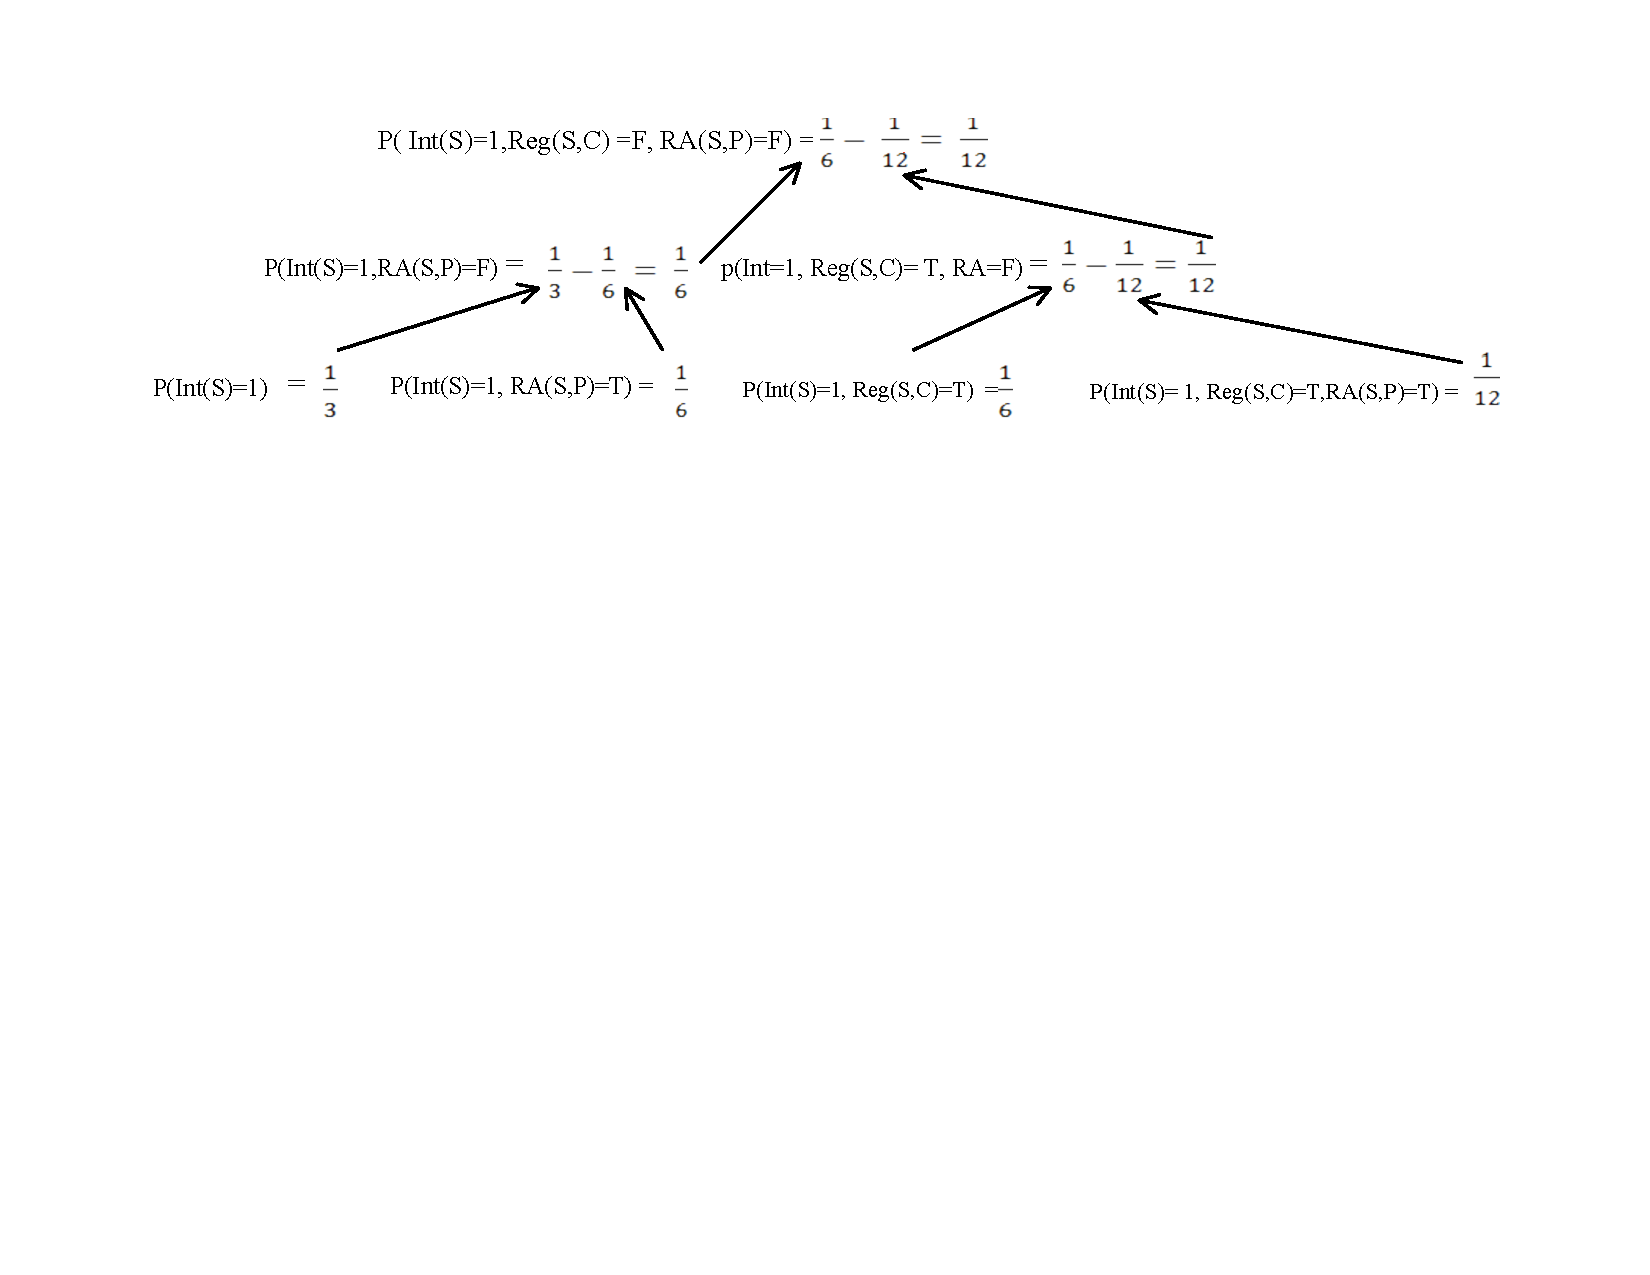
\includegraphics[width=6in]{example.pdf} 
%   \caption{To illustrate how a database frequency with %two 
%   negated relationships (nonexistent links) can be computed from frequencies that involve positive relationships (existing links) only. The leaves in the computation tree contain the M\"obius parameters that involve existing database tables only. The inverse M\"obius transform is a dynamic programming algorithm based on the recursion illustrated. To reduce clutter, we abbreviated some of the predicates. The numbers are chosen for illustration.}
%\label{fig:example}
%\end{figure*}

%\begin{algorithm}
%\begin{algorithmic}
%%{\footnotesize
%\STATE \underline{Notation}: $\r$ = Assignment for Functor Nodes; \\$\f_{\r}$= the value of 
%$f(t_{1},\ldots,t_{k})$ in row $\r$; \\ $\tau(\r)$ =  probability $\r$ stored in JP-table $\tau$. 
%\STATE \underline{Input}: database $\D$; child variable 
%%and parent variables divided into a set $\set{\R_{1},\ldots,\R_{m}}$ of relationship predicates and a set $\set{C}$ of function terms that are not relationship predicates.
% \STATE \underline{Calls}: $\join(\set{\C}, \R_1,\cdots,  \R_k)$. Computes join frequencies conditional on relationships $\R_{1},\ldots,\R_{k}$ being true.
%\STATE \underline{Output}: Joint Probability table $\tau$ %such that the entry $\tau(\r)$ for row $\r \equiv
%%(\set{\C} = \set{\C}_{\r}, \set{\R} = \set{\R}_{\r})$ is the frequencies $P_{\D}(\set{\C} = \set{\C}_{\r}, \set{\R} = \set{\R}_{\r})$ in the database distribution $\D$.
%%}
%\end{algorithmic}
%\begin{algorithmic}[1]
%%{\small
%\STATE \COMMENT{fill in rows with no false relationships using table joins}\label{line:start-join}
%\FORALL{valid rows $r$ with no assignments of $\false$ to relationship predicates}
%\FOR{$i=0$ to $m$}
%\IF[$r$ has $m-i$ unspecified relationships]{$r$ has exactly $i$ true relationships$\R^1,..,\R^i$}
%%\STATE find $P_{\D}(\set{\C} =\set{\C}_{\r}, \set{\R} = \set{\R}_{\r})$ using $\join(\set{\C} =\set{\C}_{\r}, \set{\R} = \set{\R}_{\r})$. Store the result in $\tau(\r)$. \label{line:join}
%\STATE $\tau(\r)$ = $\join(\set{\C} =\set{\C}_{\r}, \set{\R}, \set{\R}_{\r})$.  \label{line:join}
%\ENDIF
%\ENDFOR
%\ENDFOR \label{line:end-join}
%
%\STATE \COMMENT{Recursively extend the table to JP-table entries with false relationships.}
%\FORALL{%valid 
%rows $r$ with at least one assignment of $\false$ to a relationship predicate}
%\FOR{$i=1$ to $m-1$}
%\IF[find conditional probabilities when $\R^1$ is true and when unspecified]
%{$r$ has exactly $i$ false relationships $\R^1,..,\R^i$}
%\STATE Let $\r_{\true}$ be the 
%row such that (1) $\R^1_{\r_{\true}} = \true$, (2) $\f^{R^1}_{\r_{\true}}$ is unspecified for all attributes $\f^{R^1}$ of $\R^1$, and (3) $\r_{\true}$ matches $\r$ on all other variables. 
%\STATE Let $\r_{*}$ be the %consistent 
%row that matches $\r$ on all variables $\f$ that are not $\R^1$ or an attribute of $\R^1$ and has $\R^1_{\r_{*}}$ unspecified. 
%\STATE \COMMENT{The rows $r_{*}$ and $\r_{\true}$ have one less false relationship variable than $\r$.}
%\STATE Set $\tau(\r) := \tau(\r_{*}) - \tau(r_{\true}).$ \label{line:update}
%\ENDIF
%\ENDFOR
%\ENDFOR
%%}
%\end{algorithmic}
% \caption{The inverse M\"obuis transform for parameter estimation in a Functor Bayes Net.\label{alg:adapted}}
%\end{algorithm}


\section{Evaluation} \label{sec:eval}

%\subsection{Hypotheses} 
%We investigate the following hypotheses based on the preceding theoretical analysis.
%
%\begin{enumerate}
%\item The inverse M\"obius transform provides a significant speed-up compared to a simple join approach.
%\item The query answers and parameter estimates from the maximum pseudo-likelihood values should be close to the true distribution. Predictive accuracy should increase with sample size.
%%\item With relational data, the variance of the query answers and parameter estimates exceeds the asymptotic variance for i.i.d. data in the presence of link dependencies and autocorrelations, even for large data sizes.
%\end{enumerate}
We evaluated the learning times (Section~\ref{sec:learning-times}) and quality of inference (Section~\ref{sec:inference}) of our approach to class-level semantics, as well as comparing the inference accuracy of our methods to Markov Logic Networks.  Another set of simulations evaluates the accuracy of parameter estimates (conditional probabilities). 
% For those tests, the parameters were learned from the entire database. We also evaluated models learned from portions of the database to one learned from the entire database (Section~\ref{sec:conditional-probabilities}).
All experiments were done on a QUAD CPU Q6700 with a 2.66~GHz CPU and 8~GB of RAM. The datasets and code are available on the Web \cite{bib:jbnsite}.

\subsection{Datasets} 

We used %one synthetic and 
four benchmark real-world databases, with the modifications described by Schulte and Khosravi~\cite{Schulte2012}. See that article for details.  %For more details please see the references in \cite{Khosravi2010}. %and on-line sources [pointer omitted for blind review]. 
%such as \cite{bib:jbnsite}.

%\begin{table}[thbp] \centering
%%\scalebox{0.9}{
%\begin{tabular}[c]
%{|l|r|}\hline
%    \textbf{Dataset} & \textbf{\#tuples} \\ \hline
%    %University&171\\
%    %Mutagenesis &15218\\
%    Mondial & 814 \\
%    Hepatitis &12447\\
%    Financial &17912\\
%    Movielens &82623\\\hline
%\end{tabular}
%%} % end scalebox
%\caption{Size of datasets in number of table tuples.\label{table:datasetsize}}
%\end{table}


\noindent\textbf{Mondial Database.} A geography database, featuring
one self-relationship, $\it{Borders}$, that indicates which countries border each other. The data are organized in 4 tables (2 entity tables, 2 relationship tables, and 10 descriptive attributes).

\noindent\textbf{Hepatitis Database.} A modified version of the PKDD'02 Discovery Challenge database. The data are organized in 7 tables (4 entity tables, 3 relationship tables, and 16 descriptive attributes).
%, following %we adopted the modifications of 
%Frank {\em et al.} \citeyearpar{Frank2007}. %, which includes removing tests with null values. 

\noindent\textbf{Financial} A dataset from the PKDD 1999 cup. The data are organized in 4 tables (2 entity tables, 2 relationship tables, and 13 descriptive attributes).

\noindent\textbf{MovieLens.} A dataset from the UC Irvine machine learning repository. The data are organized in 3 tables (2 entity tables, 1 relationship table, and 7 descriptive attributes). 
%\textbf{Mutagenesis Database.} A dataset widely used in ILP research. % \cite{Srinivasan1996}.  
%For a description see \cite{Khosravi2010}.

%\noindent We also conducted experiments with synthetic graphs and datasets, with similar results. We omit details because of space constraints. OS: we can put in synthetic graphs.

To obtain a Bayes net structure for each dataset, we applied the learn-and-join algorithm \cite{Schulte2012} to each database with the implementation provided by the authors. This is the state-of-the-art structure learning algorithm for FBNs;  for an objective function, it uses the pseudo-likelihood described in Section~\ref{sec:learning}. 
%The algorithm was implemented using version 4.3.9-0 of CMU's Tetrad package \cite{2008a}.  

%; the supplementary material summarizes the findings.

%
%(Compare with estimating the outcome of an election from a sample of polling station results).

%\subsection{Synthetic Data} 
%
%[We have also conducted synthetic data experiments where the true Bayes net generating the data is known. Our findings regarding our basic hypotheses are the same. We omit the details for lack of space, but include result tables in the supplementary material.] 
%
%In these synthetic-data experiments we consider the performance of inference about individual entities when the true causal structure generating the data is known.
%We modify Tetrad's random graph generator for choosing a valid
% causal model for an input schema. %The number of dependencies is set to be 2 to 3 times more than the number of nodes.
% For nodes with no parents, the parameters are assigned with probabilities close to uniform distribution. For attributes with direct causality we enforce 50\% of the rows in the conditional probability table to assign a probability over 70\% to one of the values to achieve a strong causality. We generate three types of synthetic datasets. (1) \emph{Small datasets}: University schema of Table \ref{table:university-schema} with approximately 500 tuples across all tables. (2) \emph{ Medium datasets}: Schema of Table \ref{table:university-schema} with approximately 15,000 tuples across all tables. (3) \emph{Big datasets}: Tables of Schema of Table \ref{table:university-schema},  but we extend each of the tables to have 5 descriptive attributes with approximately 50,000 tuples across all tables.
%For each dataset size (small, medium, large), we generate 5 random causal graphs. For each graph, we generate one random database, and use five fold cross validation to measure the performance of each learning algorithm. 
%
%\subsection{Results} 


\subsection{Learning Times} \label{sec:learning-times}

Table~\ref{fig:runtime} shows the run times for computing parameter values. The Complement method uses SQL queries that explicitly construct tables for the complement of relationships (tables representing tuples of {\em unrelated} entities), while the IMT  method uses the inverse M\"obius transform to compute the conditional probabilities. The IMT is faster by factors of 15--237.
%The entries on the $x$-axis are sorted by the number of parameters to be computed. The table breaks down the total learning time according to (1) the time spent on parameter that involve positive probabilities only, and (2) the time required for negated relationships. 

\begin{table}[htdp]
\caption{Learning times (sec) for algorithms that construct explicit complement tables or use the inverse M\"obius transform.\label{fig:runtime}}
\begin{center}
%\resizebox{0.5\textwidth}{!}{
\begin{tabular}{|l|r|r||r|r||r|}
\hline Database & Parameters & \#tuples & Complement & IMT & Ratio \\  \hline
Mondial & 1618 & 814&157 & \textbf{7} &22 \\
Hepatitis & 1987 &  12,447 & 18,246 & \textbf{77} & 237 \\
Financial & 10926 & 17,912 & 228,114  & \textbf{14,821} &15 \\
MovieLens & 326 & 82,623 & 2,070  & \textbf{50} & 41 \\ \hline
\end{tabular}
%}
\end{center}
\label{table:runtime}
\end{table}%


% \begin{figure}[hptb]
%\begin{center}
%\resizebox{0.5\textwidth}{!}{
%\includegraphics[width=0.5\textwidth]{runtime}
%}
%\caption{Runtime results comparing the inverse M\"obius transform vs. table joins with negated relationships.\label{fig:runtime}}
%\end{center}
%\end{figure}


\subsection{Inference}\label{sec:inference}

The evaluation of parameter learning for Bayes nets is based on query accuracy of the resulting nets~\cite{Allen2008} because
answering probabilistic queries is the basic inference task for Bayes nets. Correct parameter values will support correct query results, so long as the given Bayes net structure matches the true distribution (i.e., is an I-map).  We evaluate our algorithm by formulating random queries and comparing the results returned by our algorithm to the ground truth, the actual database frequencies.

We randomly generate queries for each dataset according to the following procedure. First, randomly choose a target node $\V$ 100 times, and go through each possible value $a$ of $\V$ such that $P(\V=a)$ is the probability to be predicted. For each value $a$, choose randomly the number $k$ of conditioning variables, ranging from 1 to 3. Make a random selection of $k$ variables $\V_{1},\ldots,\V_{k}$ and corresponding values $a_{1},\ldots,a_{k}$. The query to be answered is then $P(\V=a|\V_{1} = a_{1},\ldots,\V_{k}= a_{k}).$


As done by Getoor et al.~\cite{Getoor2001}, we evaluate queries after learning parameter values on the entire database. 
Thus the Bayes net is viewed as a statistical summary of the data rather than as generalizing from a sample. Inference is carried out using the Approximate Updater of Tetrad~\cite{2008a}.
%Standard join size estimation methods for databases are used in the same way. We compare the BN predictions with the join size estimation method of MySQL; join size estimates are converted to probability estimates by dividing by the appropriate population sizes [not done yet]. 
Figure~\ref{fig:results}(left) shows the query performance for each database.
A point ($x,y$) on a curve indicates a query such that the true probability value in the database is $x$ and the probability value estimated by the model is $y$. 
%
The Bayes net inference is close to the ideal identity line, with an average difference of less than 1\% (inset numbers).
%

\begin{figure}[hptb]
\begin{center}
%\resizebox{0.5\textwidth}{!}{
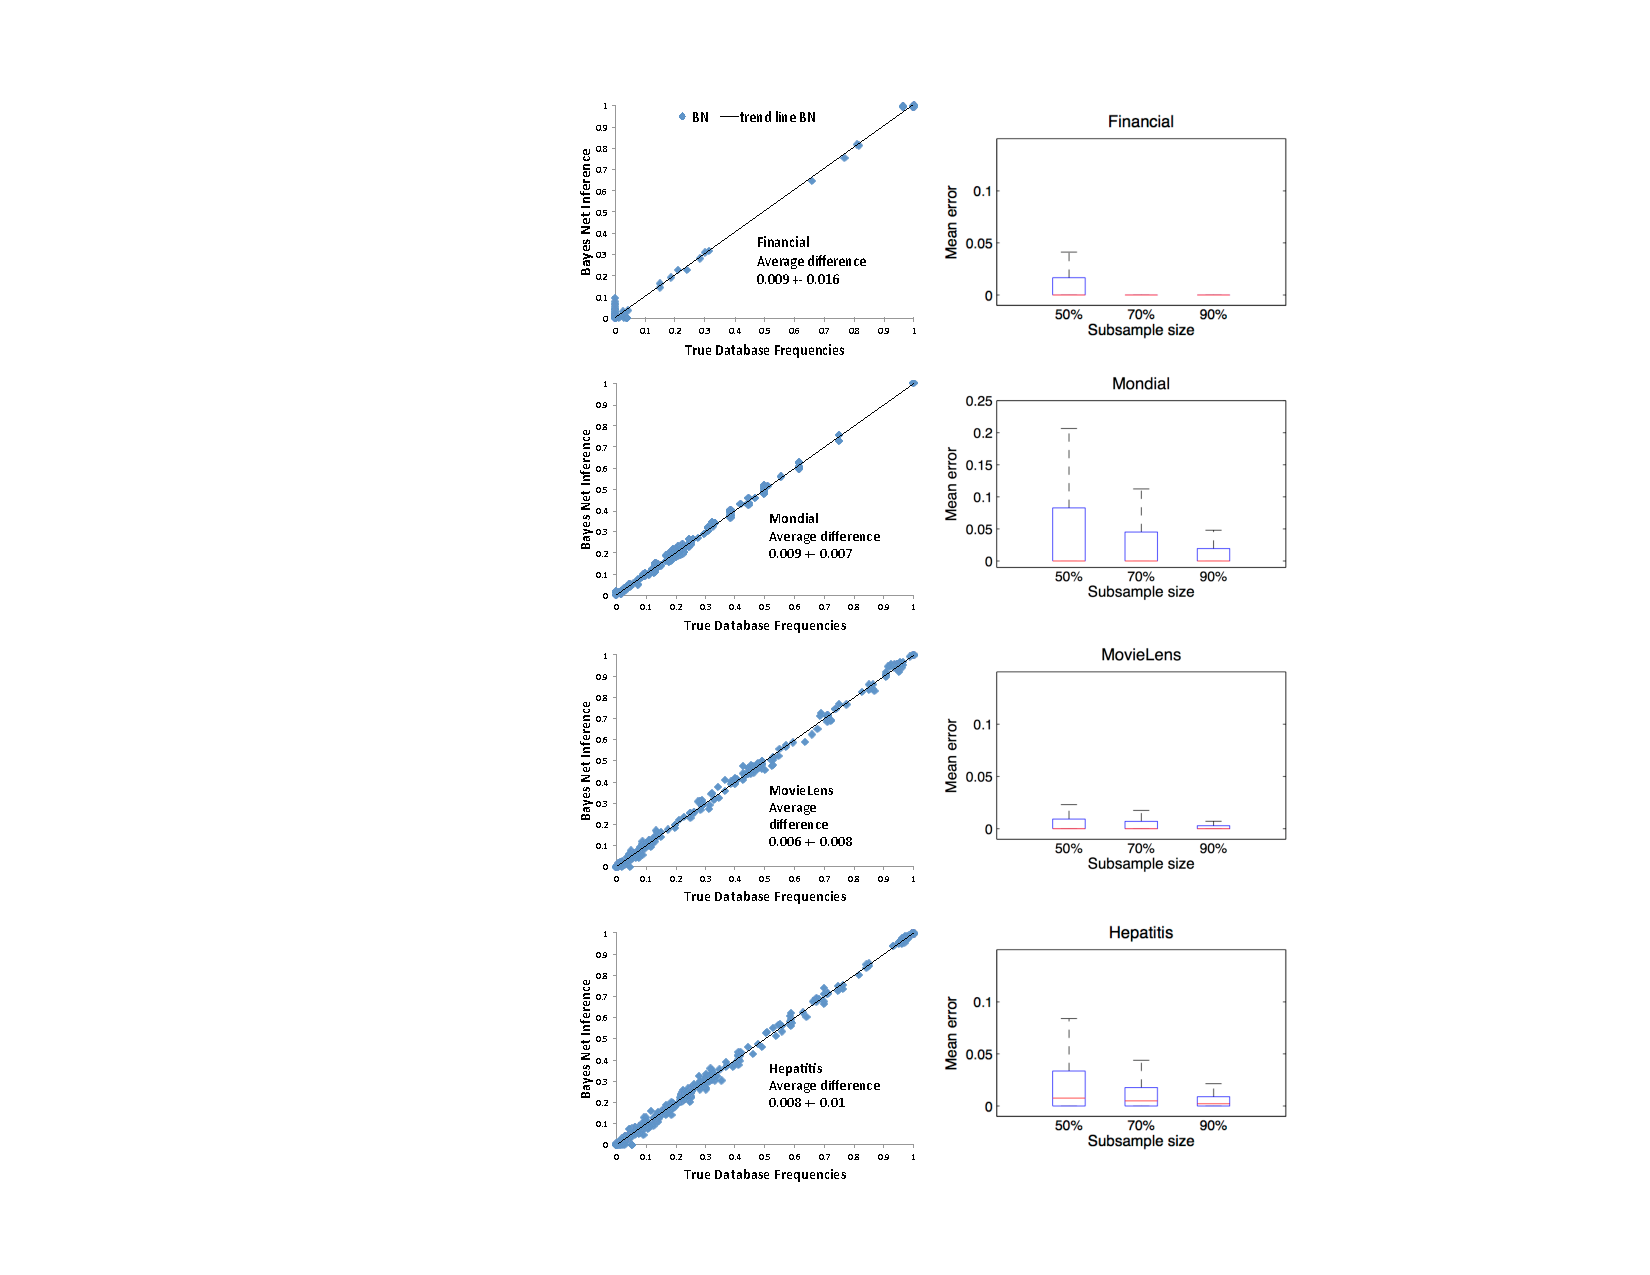
\includegraphics{figures/inf-charts-vertical.pdf}
%}
%\caption{Query Performance: Estimated vs. true probability.\label{fig:queries}}
\end{center}
\caption{{\em Left}: Query performance (Section~\ref{sec:inference}): Estimated versus true probability, with average error and standard deviation. Number of queries/average inference time per query: Mondial, 506/0.08~sec; MovieLens, 546/0.05~sec; Hepatitis, 489/0.1~sec; Financial, 140/0.02~sec. 
{\em Right:} Error (Section~\ref{sec:conditional-probabilities}): Absolute difference in estimated conditional probability parameters, averaged over 10 random subdatabases and all BN parameters. 
%
%The box contains up to the 75th percentile of observed errors, the whisker up to the 95th percentile, and the line shows the median weight size.  
Whiskers indicate the 95th percentile.
The 70\% and 90\% subsamples of the Financial database had so little variance that the whiskers are not visible. \label{fig:results}}
\end{figure}


\paragraph{Comparison With Markov Logic Networks.}

To benchmark our results, we compare the average error of FBN inferences with frequency estimates from Markov Logic Network (MLN)s. MLNs are a
good comparison point because (1) they are currently one of the most active areas of SRL research;  (2)  the Alchemy system provides an open-source, state-of-the-art implementation for learning and inference~ \cite{Kok2009a}; (3) they do not require the specification of further components (e.g., a combining rule or aggregation function); and (4) their undirected model can accommodate cyclic dependencies.
%In graphical terms, MLNs can be viewed as defining an undirected relational model. 

Like most statistical-relational models, MLNs were designed for instance-level probabilities rather than class-level queries. We therefore need an extra step to convert instance-level probabilities into class-level probabilities. To derive class-level probability estimates from instance-level inference, the following method due to Halpern \cite[fn.3]{Halpern90} can be used: Introduce a new individual constant for each first-order variable in the relational model %and its characteristics . % Actually better to cite AH94 fro Halpern's paper. Also, add more displays, white space etc.
 (e.g., random-student, random-course, and random-prof). Applying instance probability inference to these new individuals provides a query answer that can be interpreted as a class-level probability. To illustrate, if the only thing we know about Tweety is that Tweety is a bird, then the probability that Tweety flies should be the frequency of fliers in the bird population \cite{Schulte2012c}. That is, the class-level probability $P(\it{Flies}(\B) = \true)$ can be obtained from the instance-level marginal probability $P(\it{Flies}(\it{tweety}) = \true)$ where $\it{tweety}$ is a new constant not featured in the data used for learning. In the experiments below, we apply MLN inference to new constants as described to obtain class-level probability estimates.
%
We compare these learning algorithms \cite{Kok2010}:

%An MLN is applied for query frequency estimation using Halpern's method described in Section~\ref{sec:related}, which introduces a new constant for each 1st-order variable in the query (e.g. random-student for $S$, random-course for $C$, etc.). 
\noindent
\textbf{BN}: Bayes net parametrized with maximum pseudo likelihood estimates.\\
\textbf{LHL}: 
%\cite{Kok2009} 
A structure learning algorithm that produces a parametrized MLN, with Alchemy's MC-SAT for inference.\\
\textbf{LSM}: Another structure learning algorithm that produces a parametrized MLN, with Alchemy's MC-SAT for inference. In experiments by Kok and Domingos, LSM outperformed previous MLN learners.
%\cite{Kok2010}.
\\

As shown in Table~\ref{table:mln-results}, the Bayes net models provide an order of magnitude more accurate class-level estimates than the MLN models.
%This shows that even with complete-population data, constructing an accurate model of relational frequencies is nontrival.

\begin{table}[thbp] \centering
\caption{Class-level query performance of Bayes nets versus two algorithms for learning Markov Logic Networks, as indicated by average absolute error between the predicted frequency and the true database frequencies.
%The time taken for learning the structure and parameters of each of the models and also the average probability difference is given.
 %of each of the models and also the average probability difference is given. 
 NT denotes non-termination within the system resources. %($>2$ days runtime). 
}
%\scalebox{0.8}{
\begin{tabular}{|r|r|r|r|r|r|r|r|r|}
\hline & \multicolumn{3}{|c|}{Average error}\\
\hline
    Dataset & BN & MLN(LSM) & MLN(LHL)\\
\hline
    Mondial &\textbf{0.9}\% & 8.6\% &10.5\% \\
    Hepatitis &\textbf{ 0.8}\% & 11.2\% & 13.2\%\\
    Financial & \textbf{0.9}\% & 9.1\% & NT\\
    Movielens  &\textbf{0.6}\% & 14.2\% & NT\\
\hline
\end{tabular}
%} % end scalebox
\label{table:mln-results}
\end{table}


\subsection{Conditional Probabilities}\label{sec:conditional-probabilities}
%\marginpar{copy legend from SIAM or ICML}
%\begin{figure}[htbp]
%\caption{Error in conditional probability estimates. The box plots show the distribution of the absolute difference between each true conditional probability value and the estimate produced by our method, averaged over 10 random subdatabases. The center line is the median error \textbf{box meaning?} \textbf{fix ``mean'' label}
% \label{fig:cps}}
%\begin{center}
%\resizebox{1\textwidth}{!}{
%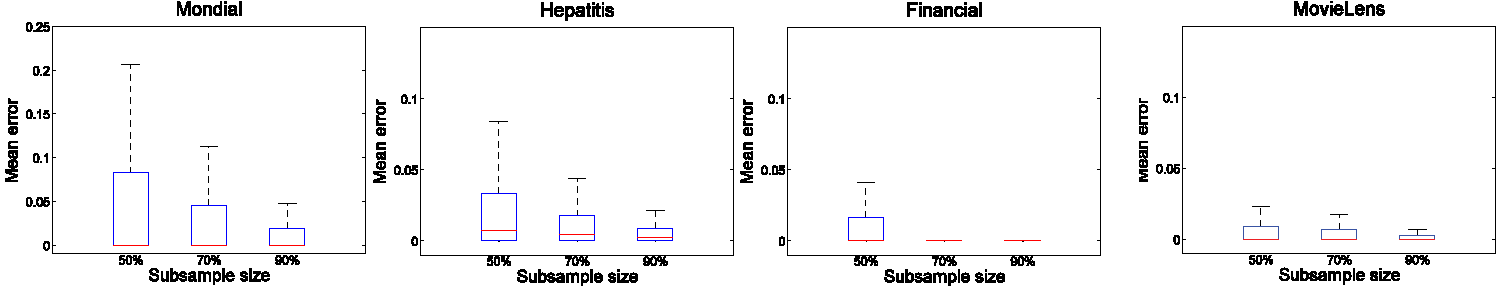
\includegraphics[width=1\textwidth]{figures/Box-plot.pdf}
%}
%%\caption{Query Performance: Estimated vs. true probability.\label{fig:queries}}
%\end{center}
%\end{figure}

In the previous inference results, the correct query answers are defined by the entire population, represented by the benchmark database, and the model is also trained on the entire database.
To study parameter estimation at different sample sizes, we trained the model on $N\%$ of the data for varying $N$ while continuing to define the correct value in terms of the entire population. 
%As in the previous section, the estimates are then compared against the true value defined by the entire population   (i.e., 100\% of the data). 
Conceptually, we treated each benchmark database as specifying an entire population, and considered the problem of estimating the complete-population frequencies from partial-population data. The $N\%$ parameter is uniform across tables and databases. 
We employed standard subgraph subsampling \cite{Frank1977,Khosravi2010}, which selects entities from each entity table uniformly at random and restricts the relationship tuples in each subdatabase to those that involve only the selected entities. Subgraph sampling provides complete link data and matches the random selection semantics. It is applicable when the observations include positive and negative link information (e.g., not listing two countries as neighbors implies that they are not neighbors). The subgraph method satisfies an ergodic law of large numbers: as the subsample size increases, the subsample relational frequencies approach the population relational frequencies. 
%For discussion of other network sampling mechanisms, please see \cite{Thompson2006}.


%These results assess the quality of parameter estimates directly. 
%As  with queries, 
The right side of Figure~\ref{fig:results} plots the difference between the true conditional probabilities and the MPLE estimates.
%The graphs distinguish between conditions with (a) autocorrelations (b) link child nodes (c) neither. 
With increasing sample size, MPLE estimates approach the true value in all cases. Even for the smaller sample sizes, the median error is close to 0, confirming that most estimates are very close to correct. As the box plots show, the 3rd quartile of estimation error is bound within 10\% on Mondial, the worst case, and within less than 5\% on the other datasets. % in the worst case, on the Mondial database with 50\% subsample size, the error rarely exceeds 5\%. 
%With training on 100\% of the data, the M\"obius transform finds the exact database 
%, and convergence is most rapid in case (c). To study the variance of parameter estimates, we use a bias-variance decomposition of the squared error averaged over subdatabases. 
%Table~\ref{table:parameter-error} shows that the observed variance constitutes a larger proportion of the observed error in cases (a) and (b). 
%plot the observed variance $x$ against the asymptotic variance for i.i.d data in Figure~\ref{fig:parameters-variance}. The asymptotic variance is a good approximation in case (c), but underestimates the observed variance in cases (a) and (b). Table \ref{table:parameter-error} shows the average ratios observed variance/lower bound. We use the ratio rather than the difference because it is less sensitive to the magnitude of the minimum variance. 

%\begin{figure}[hptb]
%\begin{center}
%\resizebox{0.5\textwidth}{!}{
%%\includegraphics[width=0.5\textwidth]{runtime}
%}
%\caption{Parameter Values: Estimated vs. true conditional probability.\label{fig:parameters}}
%\end{center}
%\end{figure}
%%
%\begin{figure}[hptb]
%\begin{center}
%\resizebox{0.5\textwidth}{!}{
%%\includegraphics[width=0.5\textwidth]{runtime}
%}
%\caption{Parameter Variances: Observed Variance vs. Nonrelational asymptotic approximation.\label{fig:parameters-variance}}
%\end{center}
%\end{figure}
%
%\begin{table}[htbp]
%\begin{center}
%\resizebox{0.5\textwidth}{!}
%{
%\begin{tabular}{|c|c|c|c|c|c|c|c|}
%\hline
%\end{tabular}
%}
%\end{center}
%\caption{Average ratio of (true parameter value/parameter estimate) per database. \label{table:parameter-error}}
%\end{table}

%\begin{figure*}[ht]
%\centering
%\hbox{
%\subfigure{
%\resizebox{0.25\textwidth}{!}{
%   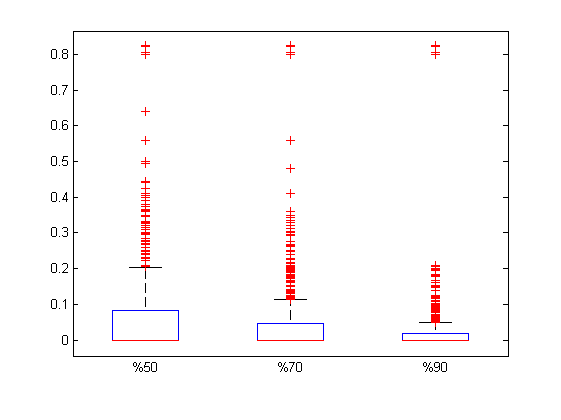
\includegraphics[width =0.25\textwidth] {mondial-box.png}
%   \label{fig:subfig1}
%   }
% }
%
% \subfigure{
%\resizebox{0.25\textwidth}{!}{
%   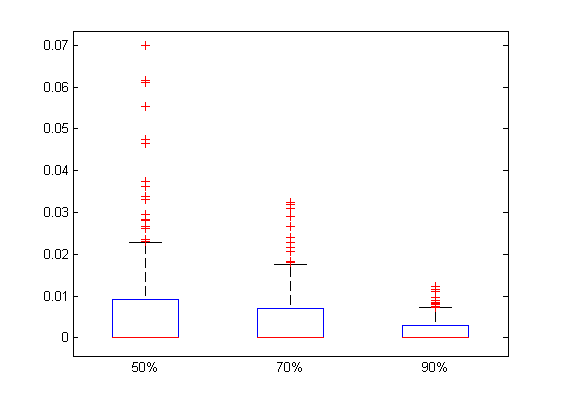
\includegraphics[width =0.25\textwidth] {movie-box.png}
%   \label{fig:subfig2}
%   }
% }
%
% \subfigure{
%\resizebox{0.25\textwidth}{!}{
%   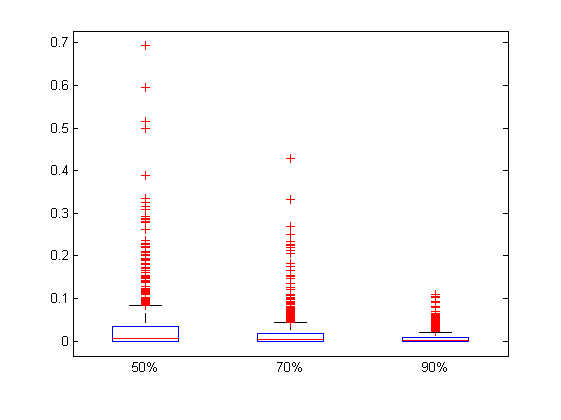
\includegraphics[width =0.25\textwidth] {hep-box.png}
%   \label{fig:subfig3}
%   }}
%   \subfigure{
%\resizebox{0.25\textwidth}{!}{
%   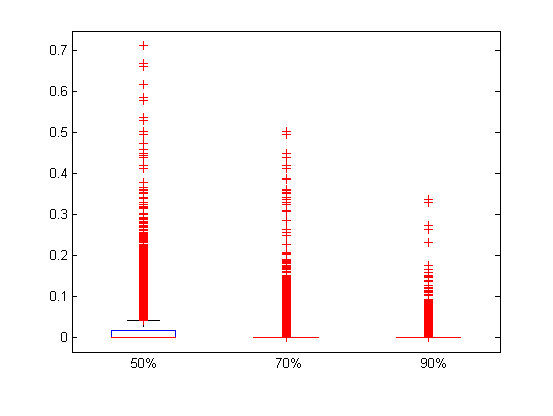
\includegraphics[width =0.25\textwidth] {fin-box.png}
%   \label{fig:subfig4}
%   }
% }
%}
% \label{myfigure}
%\caption{Global figure caption}
%\end{figure*}



%\subsubsection{Comparison With Markov Logic Networks}
%%[For example, Halpern \cite{Halpern90} showed that any instance-based inference model can be used for class-based inference as follows. Introduce a new individual constant for each first-order variable in the relational model %and its characteristics 
%% (e.g., random-student, random-course, and random-prof). Applying instance probability inference to these new individuals provides a query answer that can be interpreted as a generic frequency. To illustrate, if the only thing we know about Tweety is that Tweety is a bird, then the probability that Tweety flies should be the frequency of flyers in the bird population. In statistical terminology, marginal probabilities assigned to a ground atom should reflect population probabilities. 
%%We apply Halpern's method to perform frequency inference with Markov Logic Networks and compare it with Bayes net inference; we leave for future work comparisons with other instance probability models, such as PRMs.]
%%
%Although most statistical-relational models were designed for instance-level probabilities rather than frequency queries, Halpern's method described in Section~\ref{sec:related} allows us to apply an instance-level inference model for frequency estimates. To benchmark our results, we compare FBN inferences with Markov Logic Network (MLN) frequency estimates. In graphical terms, MLNs can be viewed as defining an undirected relational model. They are a
%good comparison point because (1) they are currently one of the most active areas of SRL research;  the Alchemy system provides open-source, state-of-the-art learning  and inference software  \cite{Kok2009a}. (2) They do not require the specification of further components (e.g., a combining rule or aggregation function). (3) An undirected model can accommodate recursive relationships (cyclic dependencies).
%We use the Alchemy's implementation of the MC-SAT algorithm for MLN inference. 
%We compare the following learning algorithms \cite{Kok2010}:
%%An MLN is applied for query frequency estimation using Halpern's method described in Section~\ref{sec:related}, which introduces a new constant for each first-order variable in the query (e.g. random-student for $S$, random-course for $C$, etc.). 
%
%\begin{description}
%\item[FBN] Bayes net parametrized with maximum pseudo likelihood estimates.
%\item[MBN+Neg] The Bayes net structure is converted to an MLN using the standard moralization procedure. The weights of clauses are learned using Alchemy's default weight learning procedure \cite{Lowd2007}. 
%%Weight learning is carried out with Alchemy, using the method of 
%%%Kok and Domingos 
%%\citet{Kok2005a}. 
%\item[LHL] The LHL algorithm 
%%\cite{Kok2009} 
%is a structure learning algorithm that produces a parametrized MLN.
%\item[LSM] The state-of-the-art LSM structure learning algorithm that produces a parametrized MLN. In experiments by Kok and Domingos, LSM outperformed other MLN learners.
%\end{description}
%
%The MBN method (for ``Moralized Bayes Net''), was used by Khosravi {\em et al.} \cite{Khosravi2010,Schulte2011b,Khosravi2012}, but {\em without clauses involving negated links}. To define a complete joint distribution for frequency querying, it is necessary to add clauses with negated links. Unfortunately, Alchemy fails to terminate on any of our datasets because of the computational challenges that arise from many clauses with negated links. This is evidence for the usefulness of the Fast M\"obius Transform. To obtain comparison results, we used state-of-the art MLN structure learning algorithms as well as the moralized structure. An advantage of this approach is that the structures are learned with Alchemy clause weight estimation as a subroutine, so they are optimized for Alchemy parameter learning.
%
%The Bayes net models provide much more accurate frequency estimates than the MLN models, with an average improvement of 10\% or more. This shows that even with complete data, learning an accurate model of relational frequencies is not a trival task.
%
%\begin{table}[thbp] \centering
%%\scalebox{0.8}{
%\begin{tabular}{|r||r||r|r|r|r|r|r|r|r|}
%\hline & \multicolumn{4}{|c|}{Average error}\\
%\hline
%    Dataset & JBN & MLN(LSM) & MLN(LHL) & MBN+Neg\\
%\hline
%    Mondial &\textbf{0.9}\% & 8.6\% &10.5\% & NT\\
%\hline
%    Hepatitis &\textbf{ 0.8}\% & 11.2\% & 13.2\% &NT\\
%\hline
%    Financial & \textbf{0.9}\% & 9.1\% & NT &NT\\
%\hline
%    Movielens  &\textbf{0.6}\% & 14.2\% & NT &NT\\
%\hline
%\end{tabular}
%%} % end scalebox
%\caption{The frequency query performance of Bayes nets vs. Markov Logic Networks. We show the average absolute error over all random queries between the predicted frequency and the true database frequencies.
%%The time taken for learning the structure and parameters of each of the models and also the average probability difference is given.
% %of each of the models and also the average probability difference is given. 
% NT denotes non-termination within the system resources. %($>2$ days runtime).
%\label{table:mln-results}}
%\end{table}
%



%\section{Frequencies and Instances} 
%
%
%%\paragraph{Type 2 Models.} 
%\label{sec:template} The majority of SRL models have been evaluated on the task of predicting individual attributes and relationships. The basic idea is to {\em ground} an FBN by instantiating its first-order variables with all possible constants.
%%, as illustrated in Figure~\ref{fig:ground} 
%%\begin{figure}[h]
%%\begin{center}
%%\resizebox{0.5\textwidth}{!}{
%%%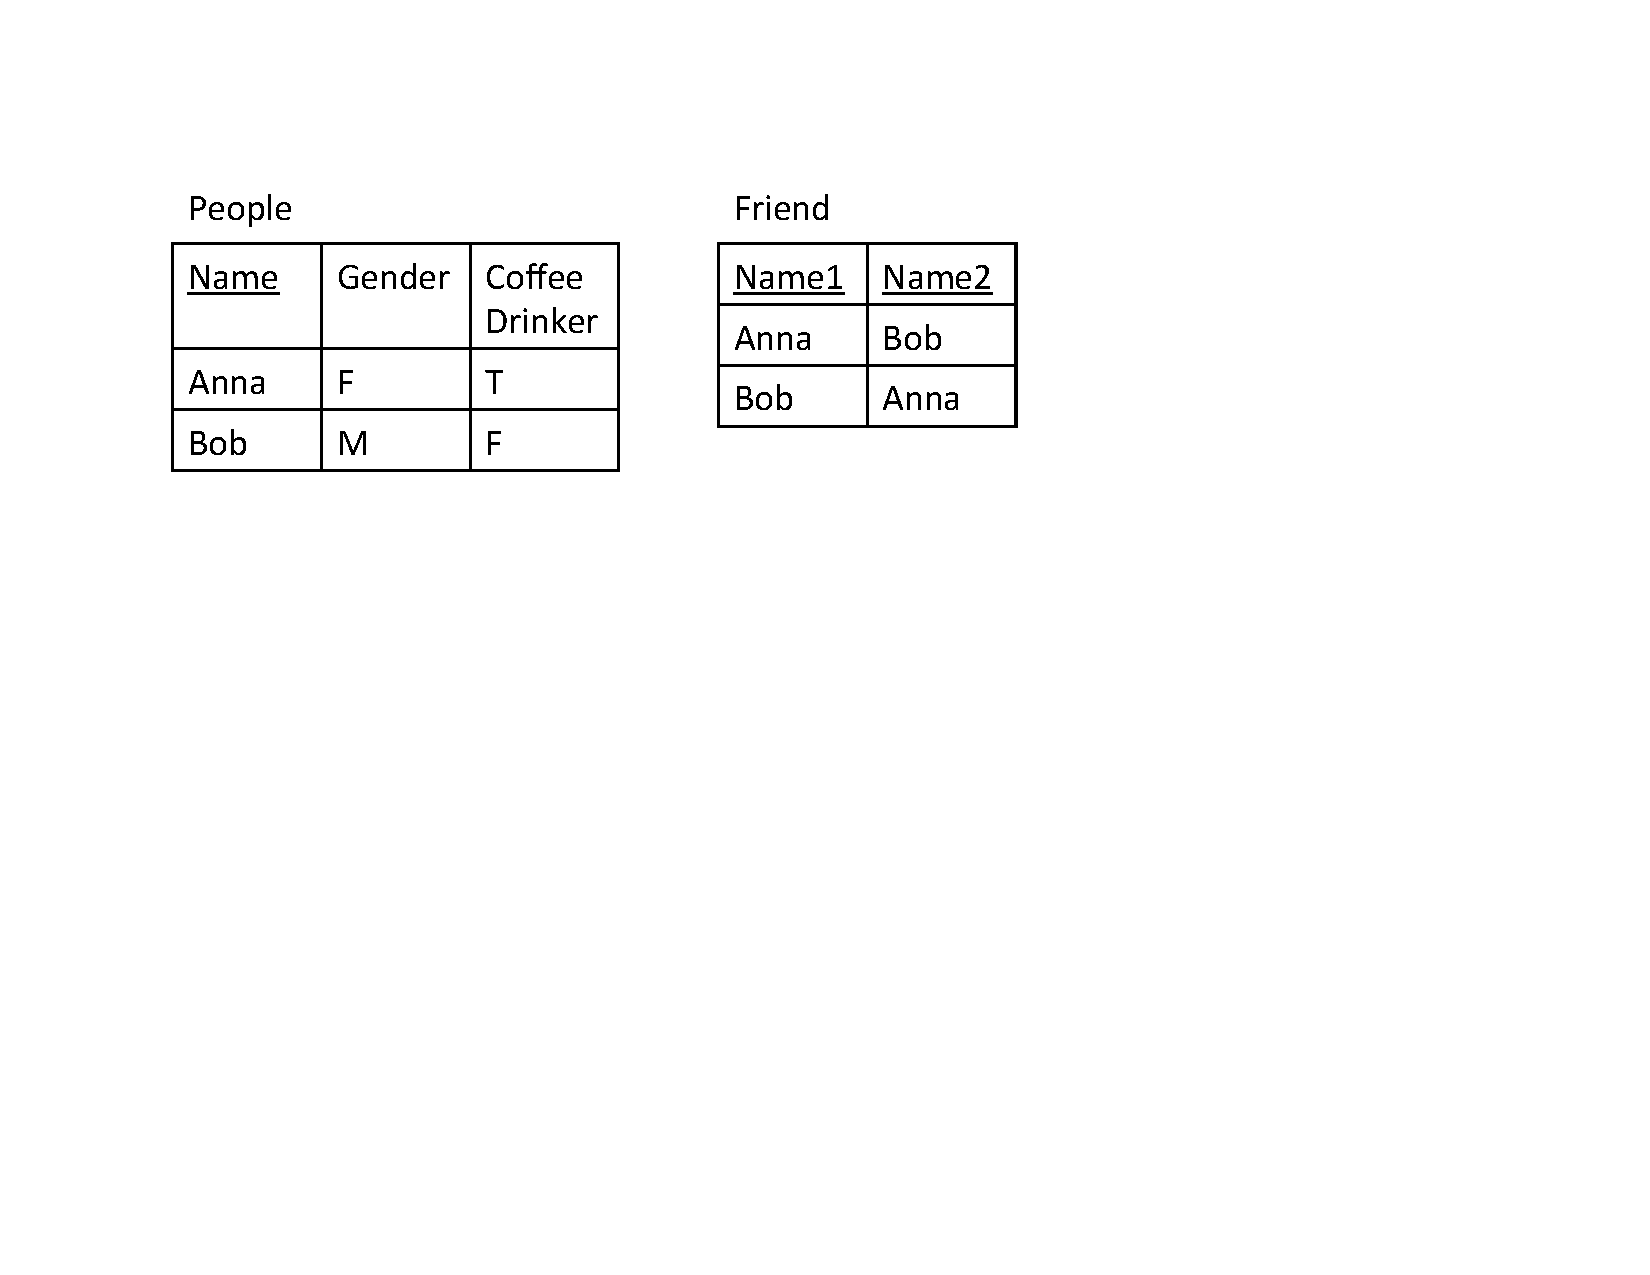
\includegraphics[width=0.5\textwidth]{db}
%%}
%%\caption{A grounding of the Bayes Net of Figure~\ref{fig:recurse}.\label{fig:ground}}
%%\end{center}
%%\end{figure}. 
%Valid reponses to type 2 queries can be defined by reference to the ground Bayes net \cite{Poole2003}. 
%%The ground model must be supplemented with a mechanism for defining the conditional probability of a ground child node given its multiple ground parents. The two main mechanisms are aggregation fuctions (e.g., average, mode) \cite{Getoor2007c,Neville2007} and combining rules (e.g., noisy-or, average) \cite{Kersting2007,Natarajan2008}. 
%%For different mechanisms, 
%Local parameter optimization methods for type 2 queries have been developed, such as gradient descent and gradient-based boosting \cite{Kersting2007,Natarajan2008,Natarajan2011}. 
%%A major problem with ground BNs is that they may contain cycles %(see Figure~\ref{fig:ground}) 
%%\cite{Neville2007}. To address this problem, 
%The moralization approach first converts the FBN to an undirected model and then carries out inference in the ground Markov model \cite{Khosravi2010}. This work made use only of the Bayes net structure, not of Bayes net parameter learning. We are not aware of any theoretical or experimental results that connect a parameter learning algorithm for type 2 inferences to database frequencies, either for bounded or limiting sample sizes.
%
%For {\em inference}, connections between relational frequencies and single-event probabilities have been a major subject in AI research \cite{Bacchus1992}. For example, Halpern discusses Miller's principle \citeyearpar{Halpern90}: Suppose that the only information we have about an individual is membership in a certain population. Then the probability assigned to the properties of the individual should be the same as the general population frequencies. Thus if we the only thing we know about Tweety is that Tweety is a bird, then the probability that Tweety flies should be the frequency of flyers in the bird population.
%We believe that a unified approach to {\em learning} for both probability types is an exciting research direction for SRL. Previous work successfully used FBN structures for type 2 inferences, and the results in this paper indicate that FBN models are also suitable for type 1 probability modelling. One possibility for unifying parameter learning is to use conditional database frequencies as parameters in type 2 directed models. Conversely, type 2 systems can be used for type 1 queries as explained by Halpern \citeyearpar{Halpern90}: Introduce a new individual constant for each first-order variable in the relational model %and its characteristics 
% (e.g., random-student, random-course, and random-prof). 
% %Because there is no other specific information available on these individuals, 
% As with Miller's principle, applying type 2 inference to these individuals using only the information specified in the query 
%provides an answer that corresponds to generic frequencies. \marginpar{results from Hassan?}
%(2) Self-relationships lead to cycles (see Figure bla), so the ground model no longer defines valid probabilistic inferences. The aim of the parameter learning methods developed for these models is to optimize type 2 queries rather than type 1. Different combining rules typically require different algorithms, for instance because they define different model score gradients [cite]. Local search methods are used; to our knowledge, there are no analytic closed-form results.
%
%Because of the difficulties with cyclic dependencies, a number of researchers have advocated the use of undirected Markov models rather than directed models. There are a number of parameter learning methods optimized for type 2 queries, for instance using gradient descent or functional gradient boosting [cite]. One of the most effective methods of learning a relational Markov model is the moralization approach: convert an FBN learned by the learn-and-join algorithm to a Markov model via the standard moralization procedure (connect coparents, omit edge directions). Type 2 inference can then be defined using the ground Markov model. The moralization procedure can be seen as deriving type 2 inferences from a FBN structure. Khosravi et al. applied obtained good performance on type 2 queries by applying previous relational Markov parameter learning procedures to the moralized Markov model. The work in this paper indicated that the pseudo-likelihood measure selects Bayes net structures that are good models of the database statistical patterns, which may well explain their good performance after moralization. However, Khosravi et al. made use only of the Bayes net structure, not of the Bayes net parameters. 

\section{Probability Logic}\label{sec:probability-logic}
First-order logic was extended to incorporate statements about probabilities
in Halpern and Bacchus's classic AI papers~\cite{Halpern90,Bacchus90}. % connecting logic and probability. 
Formalizing probability within logic provides a formal semantics for probability assertions and allows principles for probabilistic reasoning to be defined as logical axioms. This section provides a brief outline of probability logic. We describe how the random selection concept has been used to define a truth-conditional semantics for probability formulas \cite{Halpern90,Bacchus90}. This semantics is equivalent to our class-level interpretation of functor random variables. 

\subsection{Syntax} We adopt Chiang and Poole's version of predicate logic for statistical-relational modelling \cite{Chiang2012}. 
We review only the concepts that are the focus of this paper.

 Individuals are represented by {\bf constants}, which are written in lower case (e.g., $\it{bob}$). A \textbf{type} is associated with each individual, for instance $\it{bob}$ is a {\em person}. The \textbf{population} associated with type $\type$, a set of individuals, is denoted by $\population(\type)$. We assume that the populations are specified as part of the type description.
%In contrast, Bayesian Logic (BLOG)~\cite{Milch2007} extends predicate logic to an open-world setting with uncertainty about the existence or identity of individuals.
A \textbf{logical variable} is capitalized and associated with a type.  For example, the logical variable $\it{Person}$ is associated with the population $\it{person}$. We use the definition of functor given in Section~\ref{sec:relational}; we assume that the language contains functor symbols such as $\functor,\functor',g$. 
A \textbf{literal} is of the form $\functor(\term_{1},\ldots,\term_{a}) = v$, where $v$ is in the range of the functor, and each $\sigma_{i}$ is either a constant or a population variable. The types of $\term_{1},\ldots,\term_{a}$ must match the argument types of $\functor$. If all the $\term_{1},\ldots,\term_{a}$ are constants, then $\functor(\term_{1},\ldots,\term_{a}) = v$ is a \textbf{ground literal}. A ground literal is the basic unit of information. Literals can be combined to generate {\em formulas}. In this paper we consider only formulas that are \textbf{conjunctions} of literals, denoted by the Prolog-style comma notation $\functor(\term_{1},\ldots,\term_{a}) = v, \ldots,\functor'(\term'_{1},\ldots,\term'_{a'}) = v'$. The work of Halpern and Bacchus shows how to extend the random selection semantics to the full syntax of first-order logic. 

A \textbf{probability literal} is of the form 
$$
P(\formula) = p
$$
%$$
%P(\formula) = p_{1}, \ldots, P(\formula_{n}) = p_{n}
%$$
where each $p$ is a term that denotes a real number in the interval [0,1] and $\formula_{i}$ is a conjunctive formula as defined above. A probability formula is a conjunction of probability literals. We refer to predicate logic extended with probability formulas as {\em probability logic.} 


Let $\{\X_{1},\ldots,\X_{k}\}$ be a set of logical variables of types $\type_{1},\ldots,\type_{k}$. A \textbf{grounding} $\grounding$ %for $\{\X_{1},\ldots,\X_{k}\}$ 
is a set $\grounding = \{\X_{1}\backslash x_{1},\ldots,\X_{k} \backslash x_{k}\}$ where each $x_{i}$ is a constant of the same type as $\X_{i}$. A grounding $\grounding$ for a formula $\formula$ is a grounding for the variables that appear in the formula, denoted by $\formula \grounding$. 



%The \textbf{domain} of $\{\X_{1},\ldots,\X_{k}\}$ is given by
%
%$$
%\groundall_{\{\X_{1},\ldots,\X_{k}\}}\equiv \population(\type_{1}) \times \cdots \times \population(\type_{k}).
%$$
%
%The domain of an atom (formula) is the domain of the variables that appear in the atom (formula). 

\paragraph{Examples.} Consider again the social network model of Figure~\ref{fig:recurse}~(a), with a single type, $\type = \it{person}$, associated with two logical variables $\X$ and $\Y$. 
A conjunction of nonground literals is $\it{gender}(\X) = W$, $\it{gender}(\Y) = M$, $\it{Friend}(\X,\Y)=\true$. Applying the grounding $\{\X \backslash \it{anna}, \Y \backslash \it{bob}\}$ produces the conjunction of ground literals $\it{gender}(\it{anna}) = W$, $\it{gender}(\it{bob}) = M$,$\it{Friend}(\it{anna},\it{bob})=\true$. 

An example of a nonground probability formula  is $$P(\it{gender}(\X) = W,\it{gender}(\Y) = M, \it{Friend}(\X,\Y)=\true) = 1/4,$$ while an example of a ground probability formula is $$P(\it{gender}(\it{anna}) = W, \it{gender}(\it{bob}) = M,\it{Friend}(\it{anna},\it{bob})=\true) = 1/4.$$



\subsection{Semantics.} Halpern defines different semantics for probability formulas depending on whether they contain only nonground probability literals (type 1), only ground probability literals (type 2), or both (type 3). Relational statistics are represented by nonground probability formulas, so we give the formal definition for the type 1 semantics only.   
The type 2 semantics for probability formulas with ground literals is is well-known in the statistical-relational learning community \cite{Cussen2007,Milch2007},\cite[Ch.14.6.1]{Russell2010}.  An example of a mixed type 3 case is the connection between the class-level probabilities and individual marginal probabilities that we utilized in the Markov Logic Network experiments reported in Table~\ref{table:mln-results}. Schulte \cite{Schulte2012c} discusses the importance of type 3 semantics for statistical-relational learning. 

A \textbf{relational structure} $\structure$ specifies (1) a population for each type, and (2) for each functor $\functor$ a set of tuples $\structure_{\functor} = \{\langle x_{1},\ldots,x_{a},v\rangle\}$, where the tuple $\langle \x_{1},\ldots,\x_{a} \rangle$ match the functor's argument types, and the value $v$ is in the range of $\functor$. Each tuple $\langle \x_{1},\ldots,\x_{a} \rangle$ appears exactly once in $\structure_{\functor}$. 

A relational structure defines truth conditions for ground literals, conjunctive formulas, and probability formulas as follows.
 If the structure $\structure$ assigns the same value to a ground atom as a literal $\literal$, the literal is true in $\structure$, written as $\structure \models \literal$. Thus
 $$\structure \models \functor(\x_{1},\ldots,\x_{a}) = v \mbox{ iff } \langle \x_{1},\ldots,\x_{a},v \rangle \in \structure_{\functor}.$$
 A conjunction is true if all its conjuncts are true. 
All ground literals listed above are true in the structure of Figure~\ref{fig:recurse}~(b). False literals include $\it{CoffeeDrinker}(bob)$ $ = T$ and $\it{Friend}(anna,anna) = \true$.

A relational structure does not determine a truth value for a nonground literal such as $\it{gender}(\X) = M$, since a gender is not determined for a generic person $\X$. 
We follow database theory and view a nonground formula as a {\em logical query} \cite{Ullman1982}. Intuitively, the formula specifies conditions on the population variables that appear in it, and the result set lists all individuals that satisfy these conditions in a given relational structure.  Formally, we denote the formula \textbf{result set} for a structure $S$ as $\resultset_{\structure}(\formula)$, defined by

\[
\resultset_{\structure}(\formula) \equiv \{\langle \x_{1}, \ldots, \x_{k} \rangle: \structure \models \formula \{\X_{1}\backslash x_{1},\ldots,\X_{k} \backslash x_{k}\}  \rangle 
\]

To define truth conditions for nonground probability formulas, a relational structure is augmented with a distribution $P_{\type}$ over each population $\population(\type)$.  There is no constraint on the distribution. Halpern refers to such augmented structures as \textbf{type 1 relational structures}; we continue to use the symbol $S$ for type 1 structures.
Given a type 1 structure, we may view a logical variable as {\em a random selection} from its population. These random selections are independent, so for a fixed set of population variables, the population distributions induce a distribution over the groundings of the variables. The random selection semantics states that the probability of a formula in a type 1 structure is the probability of the set of groundings that satisfy the formula. In other words, it is the probability that the formula is satisfied by a randomly selected grounding. The formal definitions are as follows:


\begin{enumerate}
\item $P_{\structure}(\X_{1} = \x_{1},\ldots,\X_{a} = \x_{a}) =_{df} P_{\type_{1}}(x_{1}) \times \cdots \times P_{\type_{a}}(\x_{a})$
where $\type_{i}$ is the type of variable $\X_{i}$ and constant $\x_{i}$.
\item $\structure \models P(\formula) = p$ if and only if $p = \sum_{\langle x_{1},\ldots,x_{\a} \rangle \in \resultset_{\structure}(\formula)} P_{\structure} (\x_{1},\ldots,\x_{\a}). $
\end{enumerate}

Each joint probability specified by a functor Bayes net is a conjunction in probability logic (like Equation~\ref{eq:statement}). The net therefore specifies a set of nonground probability formulas. The logical meaning of these formulas according to the type 1 semantics is the same as the meaning of class-level probabilities according to the random selection semantics of Section~\ref{sec:class-level}. In the terminology of Bacchus, Grove, Koller, and Halpern, a set of nonground probability formulas is a {\em statistical knowledge base} \cite{Bacchus1992}. In this view, a functor Bayes net is a compact graphical representation of a statistical knowledge base, much as a small set of axioms can provide a compact representation of a logical knowledge base.


\section{Related Work and Discussion} \label{sec:related}

%\marginpar{OS:  I haven't gone over this section yet. I just moved the part on query estimation here.}
%The \emph{cardinality estimation problem} is to estimate the size of a result set, without actually retrieving the tuples in the set. Cardinality estimation is key for optimizing query processing, and has therefore been studied extensively by database researchers \cite{Babcock2005}. 
%The reason why cardinality estimation is important is that database systems process queries by breaking them into intermediate queries and combining the intermediate resultsets. Since the computational cost of retrieving and processing a resultset depends largely on its size, query planning aims to find intermediate resultsets that are as small as possible.
%
%Getoor, Taskar, and Koller \cite{Getoor2001} observed that this estimation problem is equivalent to the {\em query probability estimation problem}, defined by dividing the cardinality of a query's result set by its maximum size:

%The advantage of the probability formulation is that it casts cardinality estimation as a statistical density estimation problem. Getoor \cite{Getoor2001a} developed a Bayes net-type model for query probability estimation. % (cf. Section~\ref{sec:related}).
%Assuming that the population sizes are known, cardinality and probability estimation are clearly equivalent problems. 
%




\subsubsection{Statistical Relational Models.}  To our knowledge, the Statistical Relational Models (SRMs) of Getoor, Taskar and Koller \cite{Getoor2001a}, are the only prior statistical models with a class-level probability semantics. A direct empirical comparison is difficult as code has not been released, but
 %(Getoor, personal communication). 
SRMs have compared favorably with benchmark methods for estimating the cardinality of a database query result \cite{Getoor2001} (Sec.~\ref{sec:intro}).

SRMs differ from FBNs and other statistical-relational models in several respects. (1) SRMs are derived from a tuple semantics \cite[Def.6.3]{Getoor2001a}, which is different from the random selection semantics we propose for FBNs.
(2) SRMs are less expressive: The queries that can be formulated  using the nodes in an SRM cannot express general combinations of positive and negative relationships \cite[Def.6.6]{Getoor2001a}. This restriction stems from the fact that the SRM semantics is based on randomly selecting tuples from {\em existing tables} in the database. Complements of relationship tables are usually not stored (e.g., there is no table that lists the set of user pairs who are {\em not} friends). The expressive power of SRMs and FBNs becomes essentially equivalent if the SRM semantics is extended to include drawing random tuples from complement tables, but this
entails the large increase in storage and processing described above.
%\footnote{With complement tables included, the main difference is then that the SRM semantics randomly selects {\em tuples}, whereas Halpern's semantics randomly selects {\em individuals}. This corresponds to the difference between the tuple relational calculus and the domain relational calculus, which are known to be equivalent in expressive power \cite{Ullman1982}.}
% Can also add back in more discussion of these matters.
 %Conditional database frequencies were used by analogy with the relational case, but there was no theorem establishing these as the score maxima. 
%There is no counterpart to the result that database frequencies maximize this score \marginpar{check this} 
%nor to the consistency result for frequencies. 
%A The study by \cite{Getoor2001} used all the data for both testing and training, %(our $N\% = 100\%$ setting), 
%rather than considering increasing sample sizes. In this setting, SRMs achieved good average accuracy on the task of join selectivity estimation for random queries; the accuracy of parameter estimates was not considered.

\subsubsection{Class-level vs. Instance-level Probabilities.}
Most previous work on stat\-istical-relational learning has been concerned with instance-level probabilities for predicting the attributes and relationships of {\em individuals} \cite{getoor-intro,Russell2010}. Examples of instance-level queries include the following.

\begin{itemize}
\item Given that Tweety is a bird, what is the probability that Tweety flies?
\item Given that Sam and Hilary are friends, and given the genders of all their other friends, what is the probability that Sam and Hilary are both women?
\item What is the probability that Jack is highly intelligent given his grades?
\end{itemize}

Probability logic represents such instance-level probabilities by formulas with ground literals (e.g., $P(\it{Flies}(\it{tweety}))=p$). In graphical models, instance level probabilities are defined by a {\em template semantics}  \cite{getoor-intro}: the functors associated with every node are grounded with every appropriate constant. Instance-level probabilities can be computed by applying inference to the resulting graph.

A key difference between class- and instance-level queries is that instance-level queries can involve an unbounded number of random variables. For instance, if $\it{m}$ has 100 Facebook friends $x_{1},\ldots,x_{100}$, an instance-level query to predict the gender of $\it{m}$ given the genders of her friends would involve 200 ground literals of the form $$P(\it{gender}(\it{m})|\it{gender}(\x_{1}),\it{Friend}(\it{m},x_{1}),\ldots, \it{gender}(\x_{100}),\it{Friend}(\it{m},x_{100})).$$
In contrast,
class-level queries are restricted to the set of random variables in the class-level model, which is relatively small. For instance, the Bayes net of Figure~\ref{fig:recurse}~(b) contains four class-level random variables. This allows a query like $$P(\it{gender}(\X)|\it{gender}(\Y),\it{Friend}(\X,\Y)),$$ which predicts the gender of a single generic user, given the gender of a single generic friend. 

While we do not treat learning models for instance-level probabilities in this paper, we note that the Bayes net structures that we use in this paper also perform well for instance-level inference \cite{Schulte2012,Khosravi2010}. The structures are learned using the random selection pseudo likelihood as the main component of the objective function. These evaluations suggest the pseudo likelihood guides learning towards models that perform well for {\em both} class-level and instance-level inferences.


\subsubsection{Parfactors and Lifted Inference.} Lifted inference aims to speed up instance-level inferences by computing {\em parfactors}, that is, counts of equivalent events, rather than repeating equivalent computations \cite{Poole2003}. 
For instance, the inference procedure would count the number of male friends that $m$ has, rather than repeat the same computation for each male friend. 
Based on the similarity with computing event counts in a database, Schulte and Khosravi refer to learning with the pseudo-likelihood as {\em lifted learning}~\cite{Schulte2012}. 
%The notion of a parfactor is a key concept for efficient instance-level inference with first-order models \cite{Poole2003}. The parfactor approach shares with our work an emphasis on reasoning about class of individuals . 
The counting algorithms in this paper can likely be applied to computing parfactors that involve negated relations. The motivation for parfactors, however, is as a means to compute instance-level predictions (e.g., predict the gender of $m$). In contrast, our motivation is to learn class frequencies as an end in itself. Because parfactors are used with instance-level inferences, they usually concern classes defined with reference to specific individuals, whereas the statistics we model in this paper are at the class-level only.



\subsubsection{The Complete-Data and Closed-World Assumptions.} In logic, the closed-world assumption is that ``atomic sentences not known to be true are in fact false'' \cite[Ch.8.2.8]{Russell2010}.  While the closed-world assumption is used in logical reasoning rather than learning, it is relevant for learning if we view it as {\em an assumption about how the data are generated}. For instance, we have made the complete-data assumption that if a link between two individuals is not listed in a database, it does not exist. This entails that if a student registers in a course, this event is recorded in the university database, so the absence of a record implies that the student has not registered. If this assumption is not warranted for a particular data generating mechanism, the complete-data assumption fails, because for some pairs of individuals, the data does not indicate whether a link between does not actually exist or simply has not been recorded. One way to deal with missing link data is to  use imputation methods \cite{Hoff2007,Namata2011}. %Kleinberg too
Another approach is downsampling existing links by adding random negative links \cite{Khot2011,Yang2011}. Many methods for dealing with missing data employ complete-data learning as a subroutine (e.g., the Expectation Maximization algorithm; cf. \cite[Ch.4.3]{Domingos2009}). Given the speed and accuracy of pseudo-likelihood Bayes net learning in the complete-data case, we expect that it will be useful for learning with missing data as well.
 
Another  important point for this paper is that our methods can be used no matter how link frequencies are estimated, whether from corrected or uncorrected observed link counts. Specifically, given estimates for the M\"obius parameters, the M\"obius transform finds the probabilities for negative link events that those parameters determine. This computation assumes nothing but the laws of the probability calculus. 
% can also say something about domain closure.

%do not consider them explicitly. In classical logic, the functor-based syntax is called equational logic \marginpar{check this with David}. It can easily be converted to predicate syntax by introducing a predicate $\predicate_{\functor}$ for each functor and rewriting literals as $(\functor(\terms) = v) \rightarrow \predicate_{\functor}(\terms,v)$. Despite the equivalence to predicate logic, many, though not all, statistical formalisms for relational data are based on functions \cite{blog,Poole2003,Getoor2006,noah-goodman,pfeffer}. The main reason is that functional atoms as defined above are a natural counterpart to the statistical concept of a random variable (as we will discuss below).
%Fast Mobius transform, vs. inverse vs. zeta transform.



%For example, Halpern \cite{Halpern90} showed that any instance-based inference model can be used for class-based inference as follows. Introduce a new individual constant for each first-order variable in the relational model %and its characteristics 
% (e.g., random-student, random-course, and random-prof). Applying instance probability inference to these new individuals provides a query answer that can be interpreted as a generic frequency. To illustrate, if the only thing we know about Tweety is that Tweety is a bird, then the probability that Tweety flies should be the frequency of flyers in the bird population. In statistical terminology, marginal probabilities assigned to a ground atom should reflect population probabilities. 
%We apply Halpern's method to perform frequency inference with Markov Logic Networks and compare it with Bayes net inference; we leave for future work comparisons with other instance probability models, such as PRMs.
 
%
%While we focus on Bayes nets, the random selection semantics can be applied to any SRL model based on first-order logic, such as Markov Logic Networks. 
% 
% our results indicate that FBN models are suitable for relational frequency modelling, and previous work has used the same FBN models successfully for instance-level inferences \cite{Khosravi2010}. 

%%\cite{Bacchus1992}. 
%For example, Halpern discusses Miller's principle: Suppose that the only information we have about an individual is membership in a certain population. Then the probability assigned to the properties of the individual should be the same as the general population frequencies. Thus if we the only thing we know about Tweety is that Tweety is a bird, then the probability that Tweety flies should be the frequency of flyers in the bird population.
%We believe that a unified approach to {\em learning} for both probability types is an exciting research direction for SRL. Previous work successfully used FBN structures for type 2 inferences, and the results in this paper indicate that FBN models are also suitable for type 1 probability modelling. One possibility for unifying parameter learning is to use conditional database frequencies as parameters in type 2 directed models. Conversely, type 2 systems can be used for type 1 queries as explained by Halpern \citeyearpar{Halpern90}: 
%; we discuss this below. 
%
%\paragraph{Unified Learning for Type 1 and Type 2 Probabilities.} Previous work used different models for the two basic types of probability query (SRMs for class-level, template models for instance-level). In this paper we employ FBNs and the pseudo likelihood to learn models that are accurate for class-level probabilities. Previous research employed the same model class and objective function for learning models that are accurate for instance-level probabilities \cite{Khosravi2010,Schulte2011}. These findings indicate that learning accurate class-level probabilities leads to accurate instance-level predictions. We believe that a unified approach to learning for both relational probability types is an exciting research direction for statistical-relational learning. 
%\marginpar{add diagram about previous work?}




\section{Conclusion} Class-level probabilities represent relational statistics about the frequencies or rates of generic events and patterns. Representing these probabilities has been a long-standing concern of AI research. Class-level probabilities represent informative statistical dependencies in a relational structure, supporting such applications as strategic planning and query optimization. 
%This research generalized the concept of single-table frequencies to the relational domain: the frequency of a first-order formula in a relational database is the number of instantiations of the variables in the formula that satisfy the formula in the database, divided by the number of all possible instantiations. This frequency concept corresponds to the random selection semantics, which introduces population variables that select an individual from the given population. Attributes and links are then treated as functions of these random selections. The random selection semantics provides a foundation for generalizing single-population statistical techniques to the relational multi-population case. 
%With the random selection semantics, Bayes nets can support efficient, accurate learning and inference of class-level probabilities 
%using 
%%grounding-free semantics and 
%the Inverse M\"obius transform for learning the joint probabilities.
%This paper considered parameter learning for functor Bayes nets that model database statistics. 
%We introduced a new grounding-free semantics that supports using Bayes nets for class-level queries. 
The class-level interpretation of Bayes nets is based on the classic random selection semantics for probability logic. 
Parameters are learned using the empirical frequencies, which are the maxima of a pseudo-likelihood function. The inverse M\"obius transform makes the computation of database frequencies feasible even when the frequencies involve negated links. 
%The parameters for Bayes nets modelling a database of relations can be accurately and efficiently learned using the maximum pseudo-likelihood estimator.  
%Bayes nets can be interpreted as models of class-level statistics in a relational structure. The class-level interpretation is based on the classic random selection semantics for probability logic. 
%Our results indicate that functor Bayes nets together with maximum pseudo-likelihood estimates provide an accurate tractable model of the frequency of events in a relational structure.
%For parameter learning we utilized the empirical joint frequencies, which can be feasibly computed using the inverse M\"obius transform, even for frequencies concerning negated links.
%[0) inverse Mobius transform is fast, makes it feasible to do estimation using negated links. 1) highly accurate compared to other methods. 2) Variance is higher due to data dependencies. Future work: better understanding of variance, e.g. asymptotic approximation, or graph total paper.]
%This paper considered some of the classical results for Bayes net parameter estimation in the relational context, starting with a pseudo-likelihood function derived from the random selection semantics. 
In evaluation on four benchmark databases, the maximum pseudo-likelihood estimates approach the true conditional probabilities as observations increase. The fit is good even for medium data sizes. 
Overall, our simulations show that Bayes net models derived with maximum pseudo-likelihood parameter estimates provide excellent estimates of class-level probabilities.
% and should be applicable across a wide range of applications.

\section*{Acknowledgements} This research was supported by an NSERC Discovery Grant to Schulte. Lise Getoor's work on Statistical Relational Models inspired us to consider class-level modelling with Parametrized Bayes nets; we thank her for helpful comments and encouragement.  Preliminary versions of this paper were presented at the SRL workshop at ICML 2012 and the ILP 2012 conference. We thank the organizers for providing a discussion venue, and the referees for constructive criticism.
%Previous research indicates that the same Bayes net models also lead to state-of-the-art instance-level inferences \cite{Schulte2012}. Indeed, we would argue that we obtain good perfomance on instance-level prediction {\em because} the learned Bayes net structures are good models of class-level probabilities. Intuitively, if a model is wrong about the  general domain dependencies, it is likely to be wrong about individual dependencies as well. For example, suppose that a model posists that grades and the difficulty of a course are generally negatively correlated, when in fact they are positively correlated. This model will not give accurate predictions when we query the model to predict the difficulty of a specific course, given the grades that students have obtained in that course. Therefore aligning class-level and instance-level probabilities is a desirable goal for statistical-relational modelling.
%Bayes net predictions outperformed a standard database join size prediction method.
%selectivity method. 
%Theoretical considerations and empirical results show that the efficiency (low variance) of the estimator decreases with the presence of dependencies among links and/or linked units. 
%In the presence of such dependencies, the efficiency is less than for non relational data. 
%Relational data raise the new computational challenge of computing sufficient statistics for negated relationships. We presented a novel application of the inverse M\"obius  transform that provides a solution. 
%
%A direction for future work is to adapt more techniques from propositional i.i.d. Bayes net parameter learning, such as smoothing frequencies and incorporating uncertainty in parameter estimates \cite{Allen2008}. A theoretical understanding of estimator variance would be desirable: we may adapt the asymptotic approximations of \cite{Allen2008}, or 
%%Closed-form approximate expressions for the variance of frequency estimates in relational data would be desirable; one possible avenue is 
%apply graph estimator theory \cite{Frank1977}. 
%Halpern \cite{Halpern90} showed that any instance-level inference model can be used for class-level inference by using ground queries that contain new constants only (e.g., random-student, random-course, and random-prof). We plan to use this scheme to evaluate instance-level models, such as Markov Logic Networks, for class-level queries.
%A plausible hypothesis is that recursive dependencies of an attribute on itself lower the effective sample size and hence increase the parameter variance.
% For instance, central limit theorems are available for some data dependencies such as time series [cite Lehman]. A CLT for relational data could lead to an asymptotic variance analysis. (3) Exploring connections between learning to answer probabilistic queries concerning individual properties and learning to answer frequency queries about generic events. Is it possible to learn a single model from data that provides accurate estimates for both?
\bibliography{master}
\bibliographystyle{splncs}

\end{document}



%\begin{figure}[hptb]
%\begin{center}
%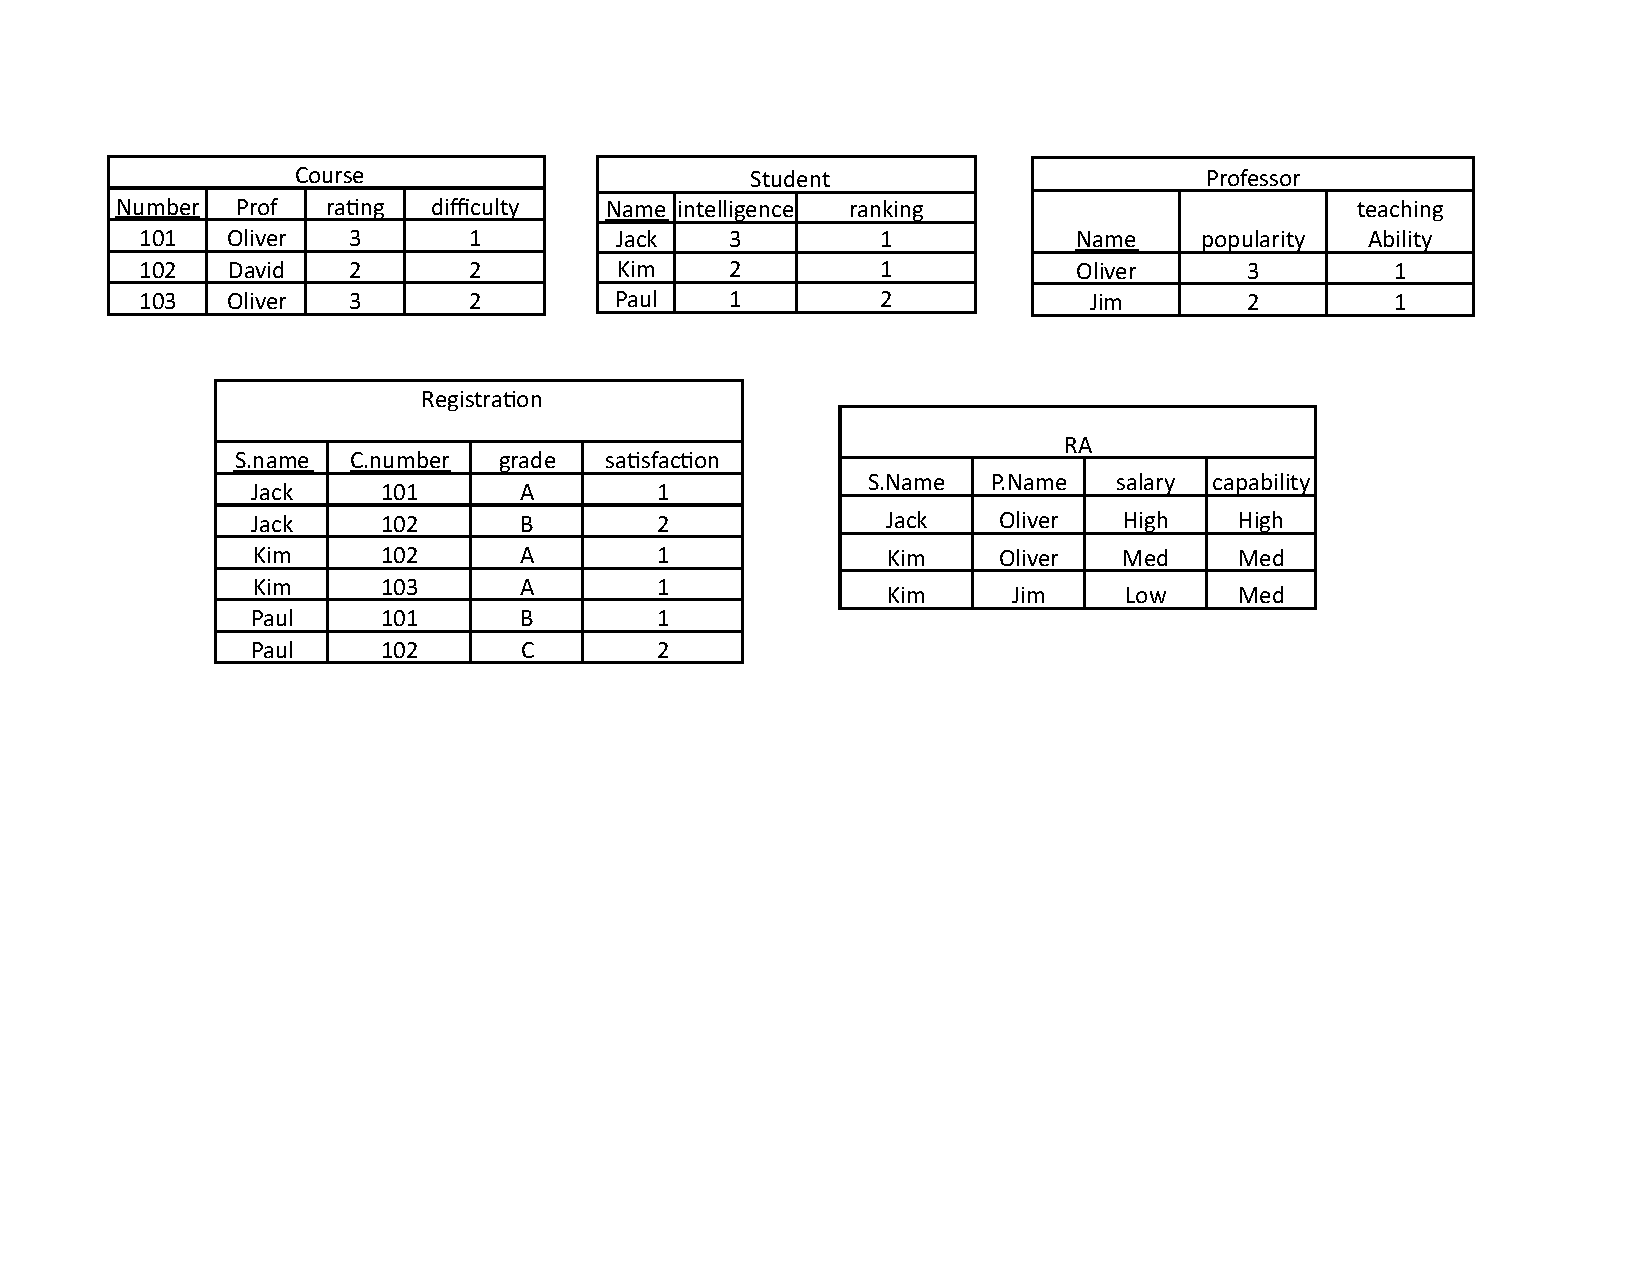
\includegraphics[width=1\textwidth]{figures/db.pdf}
%\caption{Database tables specifying a relational structure. By convention, pairs of individuals who are not listed in the the \it{Friend} table are not friends (e.g., $\it{anna,anna}).$ \label{fig:db}.}
%\end{center}
%\end{figure}


%The functor formalism translates into
% %the constraints of 
% an entity-relationship database schema \cite{Ullman1982} as follows. For simplicity, we assume that functors have at most two arguments, and that functors with two arguments are predicates, that is, binary relationships. For each population, introduce an entity table listing the members of the population. The requirement that each population member is denoted by a unique constant is called a primary key constraint in database theory, and the unique names assumption in logic [cite Russell and Norvig]. The entity table lists also the values of each descriptive attribute (unary functors), for each entity. For each binary relationship, list the pairs for which the relationship is true. By convention, if a pair is not listed, the relationship does not  hold. For example, the database instance in Figure~\ref{fig:db} signifies that $\it{anna}$ is friends with $\it{bob}$ but not with $\it{sam}$. The motivation for this convention is that the number of pairs for which the relationship does not hold is typically very large, so it is important not to store them explicitly. (For instance, the number of user pairs who are {\em not} friends on Facebook is astronomical.) The convention that if a tuple is not explicitly listed as satisfying a predicate, then it does not satisfy the predicate is called the {\em closed-world assumption} in logic (and database theory?). \marginpar{check Russell and Norvig} 
% 
%Relational structures can also be represented with annotated network graphs (Russell and Norvig), as shown in (right side of Figure).
 
%For a given relational structure, a ground literal has a probability of 100\%. A ground formula with probability less than 100\%, such as $P(\it{gender}(\it{bob}) = M) = 50\%$, expresses uncertainty about which relational structure is correct. This uncertainty can be represented by a distribution $\mu$ that assigns a probability to each relational structure \cite{Halpern90}. The probability of a grounded formula is then the probability of the set of structures in which the formula is true:
%
%\[
%\mu \models P(\formula) = p \mbox{ where } p =  \sum_{\structure: \structure \models \formula} \mu(\structure)
%\]
%
%We refer to the probabilities defined by ground probability formulas as \textbf{instance-level probabilities} since they concern instances of types.

%%
%One approach to truth-conditional semantics for such formulas in classical logic is to view them as universally quantified [cite]. For the purposes of this paper, it is useful instead to 
%

An example of a nonground probability formula is $P(\it{Flies}(B) = \true) = 90\%$, and an example of a ground probability formula is $P(\it{Flies}(\it{tweety}) = 90\%$.

%
%A \textbf{functor} represents a mapping
%$
%\functor: \indomain_{\functor} \rightarrow \outdomain_{\functor}
%$
%where $\functor$ is the name of the functor, $\indomain_{\functor} \equiv \population(\type_{1}) \times \ldots \times \population(\type_{a})$ is the {\em domain of the relation}, and $\type_{1},\ldots,\type_{a}$ are the {\em argument types} of the functor. The output type or {\em range} of the functor is denoted by $\outdomain_{\functor}$. In this paper we consider only functors with a finite range, disjoint from all populations.  If $\outdomain_{\functor} = \{\true,\false\}$, the functor $\functor$ is a (Boolean) \textbf{predicate}; other functors are called \textbf{attributes}. A predicate with more than one argument is called a \textbf{relationship}.
%In statistics, a Boolean predicate is called an indicator function. 


%An \textbf{atom} is an expression of the form $\functor(\term_{1},\ldots,\term_{a})$, where $\functor$ is a functor and each $\sigma_{i}$ is either a constant or a population variable \cite{Chiang2012}. The types of $\term_{1},\ldots,\term_{a}$ must match the argument types of $\functor$. 

Less well-known is Halpern's \textbf{random selection semantics} semantics for nonground literals.
 
 
%
%For a single population, a distribution over population members induces a joint distribution over their attributes (e.g., age, height, gender). 
%Classic AI research generalized the concept of single population frequencies to first-order logic using
% the idea of a {\em random selection} \cite{Halpern90,Bacchus90}. We provide a brief review in the context of a functor language. For example, consider a probabilistic first-order statement using the obvious abbreviations for the Bayes net of Figure~\ref{fig:recurse}:
% \begin{equation}\label{eq:statement}
%P(\it{Friend}(X,Y) = \true, \it{gender}(\X) = M, \it{gender}(\Y) = F) = 1/4.
%\end{equation}
%
%which assigns probability 1/4 to a sentence with free first-order variables.
%\footnote{The full syntax distinguishes between free variables and variables with a probabilistic interpretation.} 
%To evaluate whether the statement \eqref{eq:statement} is true in a given interpretation $\D$, the random selection semantics assumes a distribution over the population/domain associated with each free first-order variable.  Assuming the independence of these distributions, we obtain a joint distribution over the values of population variables $\X_{1},\X_{2}, \ldots, \X_{k}$; that is, a joint distribution over tuples of individuals. The type 1 probability of a first-order statement is then the sum over all tuples that satisfy the statement, weighted by the probability of each tuple. The statement is true in an interpretation if it assigns the type 1 probability correct for the interpretation. 
%
%In learning, an observed database instance $\D$ provides data only for a subpopulation. We define the \textbf{observed database frequency}, denoted by $P_{\D}$, of a functor node assignment to be the number of instantiations of the population variables in the functor nodes that satisfy the assignment in the database, divided by the number of all possible instantiations. The database frequency is the special case of the type 1 probability with a uniform distribution over all observed population members in the database. 
%%In the simplest case, the population distributions are uniform. Then the We denote this empirical joint distribution by $P_{\D}$. 
%For example, the probability statement~\eqref{eq:statement} is true in the database of Figure~\ref{fig:recurse} given a uniform distribution over users.

%\cite{Halpern90,Bacchus90,Bacchus93}. We review the random selection semantics briefly in the context of a functor language; extensive treatment in general first-order logic was provided by Halpern and Bacchus \cite{Halpern90,Bacchus90}. 
%For multiple populations, assume a distribution over each. 
%%This induces a joint distribution over the attributes of and links among the population members as follows. 
%%The key idea  is to view a population variable as a random variable that selects a member of its population. 
%Different population variables are assumed to be mutually independent, so we obtain a joint distribution over the values of population variables $\X_{1},\X_{2}, \ldots, \X_{k}$; that is, a joint distribution over tuples of individuals. Now a functor node $\functor(\X_{1},\X_{2}, \ldots, \X_{k})$ denotes a function whose arguments are population variables. So we can view it as a function of a sample drawn from the (multi)-population distribution. Since a function of random variables is itself a random variable, a distribution over population variables defines a distribution over functor nodes. If each population distribution is the uniform distribution over population members listed in a database $\D$, the resulting joint functor node distribution is the empirical database distribution $P_{\D}$. 
%Poole mentions that t

%The random selection concept provides a class-level semantics for functor Bayes nets: if we view first-order variables $\X_{1},\X_{2}, \ldots, \X_{k}$ as independent random variables that each sample an individual, then a functor of the form $\functor(\X_{1},\X_{2}, \ldots, \X_{k})$ represents a function of a random $k$-tuple. Since a function of a random variable is itself a random variable, this shows how we can view functor nodes containing first-order variables as random variables in their own right, without grounding the variables first.
%%(We discuss a template/grounding semantics in Section~\ref{sec:template}.) 
% For example, using the obvious abbreviations for the BN of Figure~\ref{fig:recurse}, the semantics of a joint assignment like 
% 
%%\begin{scriptsize}
%$$P(\it{F}(\X,\Y) = \true, \it{G}(\X) = M, \it{G}(\Y) = M, CD(\X) = \true) = 10\%$$ 
%%\end{scriptsize}
%is ``if we randomly select two users $\X$ and $\Y$, there is a 10\% chance that they are friends, both are men, and one is a coffee drinker''.    
%
%\paragraph{Random Selection Pseudo-Likelihood.}
%
%Schulte \cite{Schulte2011,Schulte2011b} proposed a way to measure the fit of a Bayes net model to relational data that matches the random selection semantics. The pseudo log-likelihood for a database $\D$ given a FBN $\B$ is the expected log-likelihood of a random instantiation of the first-order variables in the FBN with values individuals and values from the database $\D$. For a fixed database $\D$ and Bayes net structure, the parameter values that maximize the pseudo-likelihood are the \textbf{MPLE} values. These are the conditional empirical frequencies defined by the database distribution $P_{\D}$ \cite[Prop.3.1]{Schulte2011}. This result is exactly analogous to  maximum likelihood estimation for i.i.d. data. 
%%
%%: the idea is to consider a {\em random} grounding of the first-order variables in the functor Bayes net, rather than a complete grounding. 
%In the remainder of the paper we evaluate MPLE parameter estimates. We begin with a procedure for computing them.



% Conjunctive formulas correspond to theta join (joins with selection conditions), a key class of queries for query optimization [cite cowzone].
%If we extend our predicate logic with disjunctions, and restrict negations in a natural way, we obtain a logical query language known as the {\em safe domain relational calculus} \cite{Ullman1982}. 
%\marginpar{check DRC definition}
%A fundamental result of database theory states that the result sets definable in the safe domain relational calculus are exactly the same as those definable in standard relational algebra, using table joins.
%, and hence the same as those definable in SQL (without aggregate functions). 
%
% The queries (resultsets) that can be defined in the domain relational calculus are a superset of those that can be defined by standard relational algebra (with operators like the table join), and hence a superset of those that can be defined in the Structured Query Language (SQL) (excluding aggregate operators). The reason is that we can write a logical query like $\it{Friend}(\X,\Y) = \false$, which returns the set of pairs that are not friends, and hence pairs that are not listed in the given relational structure. A natural syntactic restriction on such queries defines a subset of the query language known as the safe domain relational calculus. A fundamental result of database theory is that the safe domain relational calculus is expressive equivalent to relational algebra [cite].

%
% The formal definition is as follows.
%
%\begin{enumerate}
%\item $\structure \models \functor(\x_{1},\ldots,\x_{a}) = v$ iff $\langle \x_{1},\ldots,\x_{a},v \rangle \in \structure_{\functor}$
%\item  $\structure \models \literal_{1}, \ldots, \literal_{n}$ iff $\structure \models \literal_{1}$ and ... and $\structure \models \literal_{n}$.
%\end{enumerate}
%If the populations associated with a type are not fixed with the language specification, they are specified by the relational structure (Russell and Norvig, Blog)..
%Depending on the intended application, a relational structure is also called a possible world, an interpretation, a heterogenous network, or a database instance. \marginpar{check Russell and Norvig} 
%
%\subsection{Mixed Probability Formulas.} \label{sec:instance2class} Probability formulas that contain both ground and nonground literals express connections between instance-level and class-level probabilities. Halpern investigated general connections between the two probability types \cite{Halpern90}. An example would be the axiom schema
%\[
%P(\it{Flies}(\B)) = p \leftrightarrow P(\it{Flies}(b) = p)
%\]
%where $\leftrightarrow$ is shorthand for two implications in each direction, and $\B$ and $b$ are from the same class (Birds). Intuitively, this equivalence says that if the only thing we know about an individual $b$ is that $b$ is a bird, then the probability that the individual flies is the proportion of birds that fly. Schulte argues that this equivalence principle is valid for statistical-relational inference, and leads to useful constraints on model structures and parameters \cite{Schulte2012c}. The equivalence principle can be operationalized with a statistical-relational system as follows. (1) Learn a model from relational data. (2) Introduce a new constant that denotes an individual that has not been observed in the data (e.g., $\it{new\_person}$). (3) Apply inference to query the marginal probability that the new individual has a property (e.g., $P(\it{gender}(\it{new\_person}) = M?$). Because the new person is not linked to any other individuals, the answer to this query should be the frequency with which the property holds in the individual's population (e.g., the frequency of men). This construction provides a {\em method for querying an instance-level inference system to obtain class-level probabilities} \cite{Halpern90}. We use it below to compare Markov Logic Network predictions with class-level frequencies.
%
%We believe that a unified approach to both instance-level and class-level probabilities is an exciting direction for statistical-relational learning. In the next section we show how a graphical model can support both types of queries at the same time. While our treatment focuses on Bayes nets, it also applies to other logic-based graphical models, such as Markov random fields represented in Markov Logic \cite{Domingos2009}. 

%\marginpar{check Cussen, probabilistic logic programming}
%
%\subsection{Probability Logic}
%As with predicate logic, the semantics of probability logic is different for ground and nonground formulas.
%
%\subsubsection{Semantics for Ground Probability Formulas.}
%
%
%\subsubsection{Semantics for Nonground Probability Formulas.}



%
%
%\subsection{Instance-level Semantics for Bayes Nets.} \label{sec:instance-level}
%
%The most common semantics for Functor Bayes nets views them as a {\em template} for a graphical model whose nodes are ground atoms, to support instance-level inferences \cite{getoor-intro}. 
%%In Jensen and Neville's terminology, the FBN is the {\em model graph}, and the ground FBN is the {\em inference graph}. 
%A \textbf{ground} Bayes net $\ground{B}$ is a directed graph derived from $\B$ by instantiating the population variables in the functor nodes in $\B$ with all constants of the appropriate type. 
%%Figure~\ref{fig:pbn} illustrates a Parametrized Bayes Net for the dataset in Figure \ref{fig:db-tables} and its grounding. 
%Via the product formula, the inference graph specifies a joint probability to each assignment of values to the ground atoms. Since a relational structure specifies a value for each ground atom, the set of joint value assignments stands in 1-1 correspondence with the set of relational structures. Therefore {\em the ground graph defines a probability distribution $\mu$ over relational structures}. 
%%Thus the template semantics provides a computational mechanisms for specifying the distribution $\mu$ that probability logic requires for instance-level inferences. Figure~\ref{fig:instance-semantics} illustrates the construction.
%
%A well-known problem for Bayes net template semantics arises in the presence of recursive dependencies or autocorrelations, where the value of an attribute depends on the values of the same attribute for related entities \cite{Neville2007}. In this case the ground graph often contains cycles. For example, the ground inference graph for Figure~\ref{fig:recurse} contains an edge $\it{gender}(\it{anna}) \rightarrow \it{gender}(\it{bob})$ as well as an edge $\it{gender}(\it{anna}) \leftarrow \it{gender}(\it{bob})$.
%as illustrated in Figure~\ref{fig:cycles}. 
%The cyclicity problem has been difficult to solve, and several researchers have suggested modelling autocorrelations with other types of graphical models, such as Markov random fields [cite] and dependency networks [cite]. 
%A hybrid approach is to learn using Bayes nets, and convert the Bayes net to an undirected model for inference, using the standard method of moralization (marry co-parents, omit edge directions). 
%
%Setting aside the cyclicity problem, the template semantics shows how grounding a Bayes net model supports instance-level inferences. In the next section we show how applying the Bayes net product formula directly to the nonground functor nodes  supports class-level inferences. 
%
%
%\section{Background: Parametrized Bayes Nets} Our work combines concepts from relational databases and graphical models. As much as possible, we use standard notation in these different areas.
%%\subsection{Parametrized Bayes Nets} 
%%
%functor Bayes nets are a basic graphical model for relational data \cite{Poole2003}. The syntax of FBNs is as follows. 
%We assume familiarity with Bayes nets and concepts such as CP-table and I-map \cite{Pearl1988}.
%A \textbf{functor} is a function symbol or a predicate symbol. Each functor has a set of values (constants) called the \textbf{range} of the functor. 
%There are two types of functor nodes: Boolean \textbf{relationship functors} that indicate whether a relationship holds (e.g., $\it{Friend})$, and \textbf{attribute functors} that correspond to the value of an attribute (e.g., $\it{gender}$). 
%Conforming to statistical terminology, Poole refers to first-order variables as population variables.
%%A functor whose range is $\{\true,\false\}$ is a \textbf{predicate}, usually written with uppercase letters like $P,R$. 
%A \textbf{population variable} $\X$ is associated with a population, a set of individuals; in logical terminology, a type, domain, or class. A \textbf{functor random variable}  or \textbf{functor node} is of the form $\functor(\X_{1},\ldots,\X_{k})$. In this paper we assume that functor nodes contain first-order variables only (no constants). 
%%We distinguish relationship nodes and attribute nodes depending on their type of functor. 
%A \textbf{Parametrized Bayes Net} is a Bayes net whose nodes are functor nodes. In the following we often omit the prefix ``Parametrized'' and speak simply of Bayes nets. Figure~\ref{fig:recurse} shows a FBN. The syntax of FBNs is similar to that of other directed relational graphical models (cf. \cite{Poole2003}). An \textbf{instantiation} or \textbf{grounding} 
%%$\gamma$ 
%for a set of variables $\X_{1},\ldots,\X_{k}$ assigns a constant $c_{i}$
%%$\gamma(\X_{i})$ 
%from the population of $\X_{i}$ to each variable $\X_{i}$. 
%
%%, such as Bayes Logic Programs (BLPs) \cite{Kersting2007}, object-oriented Bayes nets \cite{Koller1997}, and Probabilistic Relational Model (PRMs) \cite{Getoor2007c}. 
%%Getoor and Grant discuss the applications of function concepts as a unifying language for statistical-relational modelling \cite{Getoor2006}. 
%%A \textbf{functor random variable}  or \textbf{functor node} is of the form $\functor(\X_{1},\ldots,\X_{k})$ where $\functor$ is a functor and each term $\X_{i}$ is a first-order variable or a constant. 
%%We also refer to functor random variables as \textbf{functor nodes}, or for short \textbf{fnodes}.
%%An assignment of the form $\functor(\set{X}) = \nodevalue$, where $\nodevalue$ is a constant in the range of $\functor$, is an \textbf{atom}. A \textbf{population} is a set of individuals, corresponding to a domain or type in logic. Each first-order variable $\X$ is associated with a population $\population_{\X}$ of size $|\population_{\X}|$. 
%
% The functor formalism is rich enough to represent 
% %the constraints of 
% an entity-relationship  schema
%  %\cite{Ullman1982} 
%  via the following translation: Entity sets correspond to populations, descriptive attributes to functors, relationship tables to Boolean functors, and foreign key constraints to type constraints on the arguments of relationship predicates. Figure~\ref{fig:recurse} shows a functor Bayes net and a simple relational database instance.
%
% \begin{figure}[hptb]
%\begin{center}
%\resizebox{1\textwidth}{!}{
%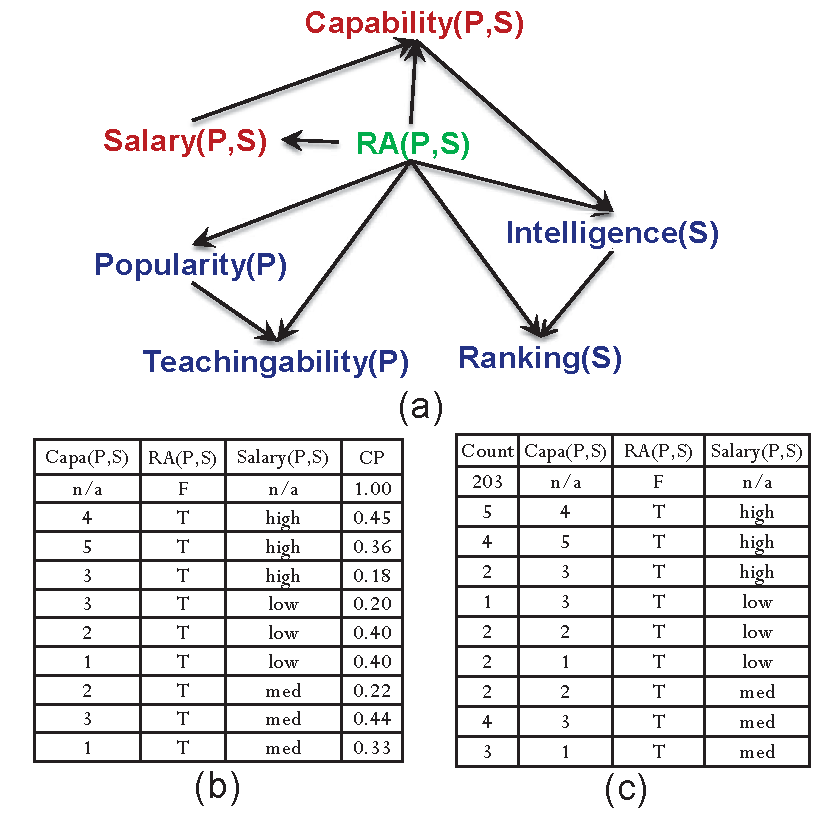
\includegraphics[width=1\textwidth]{figures/pbn.pdf}
%}
%\caption{Left: An illustrative Parametrized Bayes Net. 
%$\it{Friend}(\X,\Y)$ is a relationship node, the other three nodes are attribute nodes.
%% with an autocorrelation on the attribute $\it{gender}$.
%Right: A simple relational database instance.
%\label{fig:recurse}}
%\end{center}
%\end{figure}
%
%%
%% 
%%  \begin{figure}[h]
%%\begin{center}
%%\resizebox{0.5\textwidth}{!}{
%%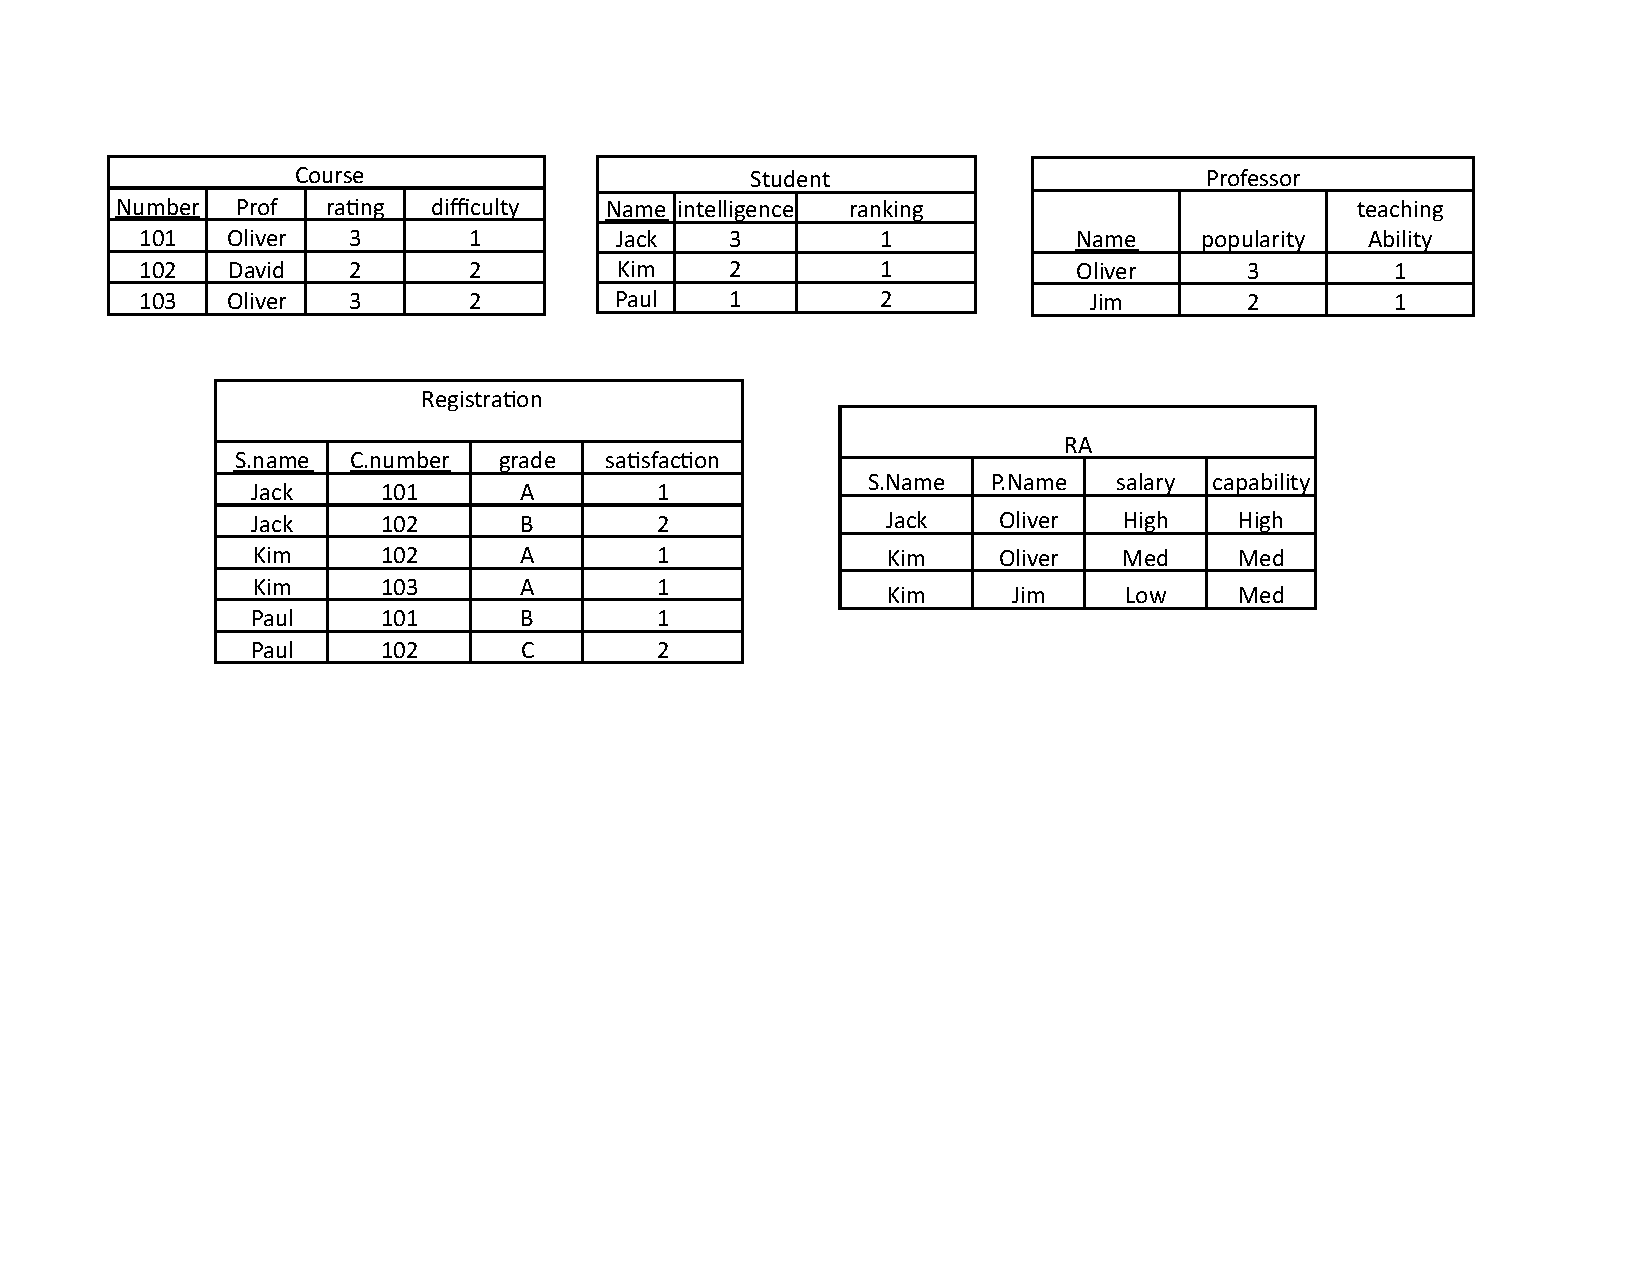
\includegraphics[width=0.5\textwidth]{figures/db.pdf}
%%}
%%\caption{A simple relational database instance.\label{fig:db-tables}}
%%\end{center}
%%\end{figure}
%
%%The \textbf{database frequency} of a functor node assignment in a relational database is the number of instantiations of the population variables in the functor nodes that satisfy the assignment in the database, divided by the number of all possible instantiations. We denote this empirical joint distribution by $P_{\D}$. For example, in the instance of Figure~\ref{fig:db-tables}, we have 
%%
%%\begin{scriptsize}
%%$$P_{\D}(\it{Friend}(X,Y) = \true, \it{gender}(\X) = M, \it{gender}(\Y) = F) = 1/4$$ 
%%\end{scriptsize}
%%since the gender conditions are met in 1 out of 4 possible instantiations of the $\X,\Y$ population variables. %, and refer to it 
%%as the \textbf{database distribution}, or \textbf{database frequency}. 
%%The following notation is useful.
%%%for parameters and database statistics. 
%%\begin{itemize}
%%\item Let $\family_{ijk}$ be the \textbf{family assignment} where $\functor_{i}$ is assigned its $k$-th value, and the state of its parents is assigned its $j$-th value.
%%\item The symbol $\theta_{ijk}$ denotes the conditional probability defined in the CP-table of the FBN for the event (parent-child state) $\family_{ijk}$.
%% \item $\instances_{ijk}(\D)$ is the number of groundings of $\family_{ijk}$ that evaluate as true in database $\D$.
%%% \item $p_{ijk} \equiv P_{\D}(\family_{ijk})$ is the frequency of a family state.
%% \end{itemize}
%%
%%\begin{table}[htbp]
%%\caption{To illustrate our notation with the database $\D$ of Figure~\ref{fig:db-tables}.}
%%\resizebox{0.5\textwidth}{!}
%%{
%%\begin{tabular}{|l|c|c|}
%%\hline
%%Family State & \multicolumn{1}{l|}{\#instances} & \multicolumn{1}{l|}{conditional probability} \\ \hline
%%$F_{ijk}$ & $n_{ijk}(\D)$ & $\theta_{ijk}$ \\ \hline\hline
%%$\it{G}(\Y) = F,\it{G}(\X)=M,\it{F}(\X,\Y) = \true$ & 1 & 0.3 \\ \hline
%%$\it{G}(\X) = F,\it{CD}(\X)=\true$ & 1 & 0.8 \\ \hline
%%\end{tabular}
%%\label{table:notation}
%%}
%%\end{table}
%
%
%%
%% For example, the semantics of an expression like 
%%\begin{scriptsize}
%%$$P(\it{Friend}(\X,\Y) = \true, \it{gender}(\X) = M, \it{gender}(\Y) = M) = 10\%$$ 
%%\end{scriptsize}
%%is ``if we randomly select two users $\X$ and $\Y$, the chance that they are friends and both men is 10\%''.   
%%
%
%
%%\subsection{Bayes Nets} We employ notation and terminology from \cite{Pearl1988,Spirtes2000} for a Bayesian Network. A {\bf Bayes net structure} is a directed acyclic graph (DAG) $G$, whose nodes comprise a set of random variables denoted by $\nodes$. We consider only discrete finite random variables.
%%When discussing a Bayes net, we refer interchangeably to its nodes or its variables.
%%The parents of node $\node_{i}$ in graph $\G$ are denoted by $\Parents_{i}$, and an assignment of values to the parents is denoted as $\parents_{i}$.
%%%The neighbors and spouses of a node $\X$ form the \textbf{Markov blanket} of $\X$.
%%%When there is  no risk of confusion, we often simply write $\parents_{\X}$.
%%A Bayes net (BN) is a pair
%%$\langle{G,\bs{\theta}_G}\rangle$ where $\bs{\theta}_G$ is a set of parameter values that specify the  probability distributions of children conditional on instantiations of their parents.
%%% i.e. all conditional probabilities of the form
%%%\[\theta_{ijk} \equiv P(\node_{i}=\nodevalue_{ik}|\Parents_{i}=\parents_{ij}),\] where $\nodevalue_{ik}$ is the $k$-th possible value of node $i$ and $\parents_{ij}$ is the $j$-th possible configuration of the parents of $\node_{i}$. 
%%The conditional probabilities are specified in a \textbf{conditional probability table} for variable $\node_{i}$ or CP-table. A \textbf{Functor Bayes net}, or FBN, is a Bayes net whose nodes are functor random variables. %
%%%A \textbf{functor Bayes net}, or FBN, is a Bayes net whose nodes are functor random variables. 
%%Poole \cite{Poole2003} refers to a functor random variable as a ``parametrized random variable'', and to an FBN as a ``Parametrized Bayes Net''. We use the term Functor Bayes Net to emphasize the use of function/predicate symbols, and to avoid confusion with the statistical sense of ``parametrized'', meaning that values have been assigned to parameters. As we discuss only FBNs in the remainder of the paper, we also speak simply of a Bayes net. \marginpar{just drop the issue?}
%%
%%The syntax of FBNs is similar to that of other directed graphical SRL models (cf. \cite{Poole2003}), such as Bayes Logic Programs (BLPs) \cite{Kersting2007}, object-oriented Bayes nets \cite{Koller1997}, and Probabilistic Relational Model (PRMs) \cite{Getoor2007c}. Getoor and Grant discuss the applications of function concepts as a unifying language for statistical-relational modelling \cite{Getoor2006}. We use FBNs for the following reasons. (1) They are a comparatively simple adaptation of the Bayes net format for relational data. (2) Standard BN inference algorithms can be applied to an FBN ``as is'', since FBNs are just Bayes nets whose nodes have a special structure.
%%
%% 

